\documentclass[12pt,a4paper,]{report}
\usepackage{lmodern}

% fix for pandoc 1.14
\providecommand{\tightlist}{%
  \setlength{\itemsep}{0pt}\setlength{\parskip}{0pt}}

% TP: hack to truncate list of figures/tables.
\usepackage{truncate}
\usepackage{caption}
\usepackage{tocloft}
% TP: end hack

\usepackage{amssymb,amsmath}
\usepackage{ifxetex,ifluatex}
\usepackage{fixltx2e} % provides \textsubscript
\ifnum 0\ifxetex 1\fi\ifluatex 1\fi=0 % if pdftex
  \usepackage[T1]{fontenc}
  \usepackage[utf8]{inputenc}
\else % if luatex or xelatex
  \ifxetex
    \usepackage{mathspec}
    \usepackage{xltxtra,xunicode}
  \else
    \usepackage{fontspec}
  \fi
  \defaultfontfeatures{Mapping=tex-text,Scale=MatchLowercase}
  \newcommand{\euro}{€}
\fi
% use upquote if available, for straight quotes in verbatim environments
\IfFileExists{upquote.sty}{\usepackage{upquote}}{}
% use microtype if available
\IfFileExists{microtype.sty}{%
\usepackage{microtype}
\UseMicrotypeSet[protrusion]{basicmath} % disable protrusion for tt fonts
}{}
\usepackage{color}
\usepackage{fancyvrb}
\newcommand{\VerbBar}{|}
\newcommand{\VERB}{\Verb[commandchars=\\\{\}]}
\DefineVerbatimEnvironment{Highlighting}{Verbatim}{commandchars=\\\{\}}
% Add ',fontsize=\small' for more characters per line
\newenvironment{Shaded}{}{}
\newcommand{\KeywordTok}[1]{\textcolor[rgb]{0.00,0.44,0.13}{\textbf{{#1}}}}
\newcommand{\DataTypeTok}[1]{\textcolor[rgb]{0.56,0.13,0.00}{{#1}}}
\newcommand{\DecValTok}[1]{\textcolor[rgb]{0.25,0.63,0.44}{{#1}}}
\newcommand{\BaseNTok}[1]{\textcolor[rgb]{0.25,0.63,0.44}{{#1}}}
\newcommand{\FloatTok}[1]{\textcolor[rgb]{0.25,0.63,0.44}{{#1}}}
\newcommand{\ConstantTok}[1]{\textcolor[rgb]{0.53,0.00,0.00}{{#1}}}
\newcommand{\CharTok}[1]{\textcolor[rgb]{0.25,0.44,0.63}{{#1}}}
\newcommand{\SpecialCharTok}[1]{\textcolor[rgb]{0.25,0.44,0.63}{{#1}}}
\newcommand{\StringTok}[1]{\textcolor[rgb]{0.25,0.44,0.63}{{#1}}}
\newcommand{\VerbatimStringTok}[1]{\textcolor[rgb]{0.25,0.44,0.63}{{#1}}}
\newcommand{\SpecialStringTok}[1]{\textcolor[rgb]{0.73,0.40,0.53}{{#1}}}
\newcommand{\ImportTok}[1]{{#1}}
\newcommand{\CommentTok}[1]{\textcolor[rgb]{0.38,0.63,0.69}{\textit{{#1}}}}
\newcommand{\DocumentationTok}[1]{\textcolor[rgb]{0.73,0.13,0.13}{\textit{{#1}}}}
\newcommand{\AnnotationTok}[1]{\textcolor[rgb]{0.38,0.63,0.69}{\textbf{\textit{{#1}}}}}
\newcommand{\CommentVarTok}[1]{\textcolor[rgb]{0.38,0.63,0.69}{\textbf{\textit{{#1}}}}}
\newcommand{\OtherTok}[1]{\textcolor[rgb]{0.00,0.44,0.13}{{#1}}}
\newcommand{\FunctionTok}[1]{\textcolor[rgb]{0.02,0.16,0.49}{{#1}}}
\newcommand{\VariableTok}[1]{\textcolor[rgb]{0.10,0.09,0.49}{{#1}}}
\newcommand{\ControlFlowTok}[1]{\textcolor[rgb]{0.00,0.44,0.13}{\textbf{{#1}}}}
\newcommand{\OperatorTok}[1]{\textcolor[rgb]{0.40,0.40,0.40}{{#1}}}
\newcommand{\BuiltInTok}[1]{{#1}}
\newcommand{\ExtensionTok}[1]{{#1}}
\newcommand{\PreprocessorTok}[1]{\textcolor[rgb]{0.74,0.48,0.00}{{#1}}}
\newcommand{\AttributeTok}[1]{\textcolor[rgb]{0.49,0.56,0.16}{{#1}}}
\newcommand{\RegionMarkerTok}[1]{{#1}}
\newcommand{\InformationTok}[1]{\textcolor[rgb]{0.38,0.63,0.69}{\textbf{\textit{{#1}}}}}
\newcommand{\WarningTok}[1]{\textcolor[rgb]{0.38,0.63,0.69}{\textbf{\textit{{#1}}}}}
\newcommand{\AlertTok}[1]{\textcolor[rgb]{1.00,0.00,0.00}{\textbf{{#1}}}}
\newcommand{\ErrorTok}[1]{\textcolor[rgb]{1.00,0.00,0.00}{\textbf{{#1}}}}
\newcommand{\NormalTok}[1]{{#1}}
\usepackage{longtable,booktabs}
\usepackage{graphicx}
\makeatletter
\def\maxwidth{\ifdim\Gin@nat@width>\linewidth\linewidth\else\Gin@nat@width\fi}
\def\maxheight{\ifdim\Gin@nat@height>\textheight\textheight\else\Gin@nat@height\fi}
\makeatother
% Scale images if necessary, so that they will not overflow the page
% margins by default, and it is still possible to overwrite the defaults
% using explicit options in \includegraphics[width, height, ...]{}
\setkeys{Gin}{width=\maxwidth,height=\maxheight,keepaspectratio}
\ifxetex
  \usepackage[setpagesize=false, % page size defined by xetex
              unicode=false, % unicode breaks when used with xetex
              xetex]{hyperref}
\else
  \usepackage[unicode=true]{hyperref}
\fi
\hypersetup{breaklinks=true,
            bookmarks=true,
            pdfauthor={},
            pdftitle={},
            colorlinks=true,
            citecolor=blue,
            urlcolor=blue,
            linkcolor=magenta,
            pdfborder={0 0 0}}
\urlstyle{same}  % don't use monospace font for urls
\setlength{\parindent}{0pt}
\setlength{\parskip}{6pt plus 2pt minus 1pt}
\setlength{\emergencystretch}{3em}  % prevent overfull lines
\setcounter{secnumdepth}{5}

\date{}


% Table of contents formatting
\renewcommand{\contentsname}{Table of Contents}
\setcounter{tocdepth}{3}

% Headers and page numbering
\usepackage{fancyhdr}
\pagestyle{plain}

% Following package is used to add background image to front page
\usepackage{wallpaper}

% Table package
\usepackage{ctable}% http://ctan.org/pkg/ctable

% Deal with 'LaTeX Error: Too many unprocessed floats.'
\usepackage{morefloats}
% or use \extrafloats{100}
% add some \clearpage

% % Chapter header
% \usepackage{titlesec, blindtext, color}
% \definecolor{gray75}{gray}{0.75}
% \newcommand{\hsp}{\hspace{20pt}}
% \titleformat{\chapter}[hang]{\Huge\bfseries}{\thechapter\hsp\textcolor{gray75}{|}\hsp}{0pt}{\Huge\bfseries}

% % Fonts and typesetting
% \setmainfont[Scale=1.1]{Helvetica}
% \setsansfont[Scale=1.1]{Verdana}

% FONTS
\usepackage{xunicode}
\usepackage{xltxtra}
\defaultfontfeatures{Mapping=tex-text} % converts LaTeX specials (``quotes'' --- dashes etc.) to unicode
% \setromanfont[Scale=1.01,Ligatures={Common},Numbers={OldStyle}]{Palatino}
% \setromanfont[Scale=1.01,Ligatures={Common},Numbers={OldStyle}]{Adobe Caslon Pro}
%Following line controls size of code chunks
% \setmonofont[Scale=0.9]{Monaco}
%Following line controls size of figure legends
% \setsansfont[Scale=1.2]{Optima Regular}

%Attempt to set math size
%First size must match the text size in the document or command will not work
%\DeclareMathSizes{display size}{text size}{script size}{scriptscript size}.
\DeclareMathSizes{12}{13}{13}{13}

% ---- CUSTOM AMPERSAND
% \newcommand{\amper}{{\fontspec[Scale=.95]{Adobe Caslon Pro}\selectfont\itshape\&}}

% HEADINGS
\usepackage{sectsty}
\usepackage[normalem]{ulem}
\sectionfont{\rmfamily\mdseries\Large}
\subsectionfont{\rmfamily\mdseries\scshape\large}
\subsubsectionfont{\rmfamily\bfseries\upshape\large}
% \sectionfont{\rmfamily\mdseries\Large}
% \subsectionfont{\rmfamily\mdseries\scshape\normalsize}
% \subsubsectionfont{\rmfamily\bfseries\upshape\normalsize}

% Set figure legends and captions to be smaller sized sans serif font
\usepackage[font={footnotesize,sf}]{caption}

\usepackage{siunitx}

% Adjust spacing between lines to 1.5
\usepackage{setspace}
% \onehalfspacing
\doublespacing
\raggedbottom

% Set margins
\usepackage[top=1.5in,bottom=1.5in,left=1.5in,right=1.4in]{geometry}
\setlength\parindent{1cm} % indent at start of paragraphs (set to 0.3?)
\setlength{\parskip}{9pt}

% Add space between pararaphs
% http://texblog.org/2012/11/07/correctly-typesetting-paragraphs-in-latex/
% \usepackage{parskip}
% \setlength{\parskip}{\baselineskip}

% Set colour of links to black so that they don't show up when printed
\usepackage{hyperref}
\hypersetup{colorlinks=true, linkcolor=black}

% Tables
\usepackage{booktabs}
\usepackage{threeparttable}
\usepackage{array}
\newcolumntype{x}[1]{%
>{\centering\arraybackslash}m{#1}}%

% Allow for long captions and float captions on opposite page of figures
% \usepackage[rightFloats, CaptionBefore]{fltpage}

% Don't let floats cross subsections
% \usepackage[section,subsection]{extraplaceins}

\begin{document}

\begin{titlepage}
    \begin{center}

    
   
        
        \vspace*{2.5cm}
        
        \huge
        The Sparse Engram of the Lateral Amygdala
        
        \vspace{1.5cm}

        by
        \vspace{1.5cm}
        
        \Large
        Dano Morrison

        \vspace{1.5cm}

        \normalsize
        A thesis presented in conformity with the requirements\\
        for the degree of \textit{Master of Science}
        
        \vfill
        
        \normalsize
        Department of Physiology\\
        University of Toronto

        \vspace{0.8cm}

        % Copyright by Dano Morrison 2016.

    \end{center}
\end{titlepage}

\vspace*{\fill}

\noindent  \textit{
I, AUTHORNAME confirm that the work presented in this thesis is my own. Where information has been derived from other sources, I confirm that this has been indicated in the thesis.
} \vspace*{\fill}

\begin{center}
\Large
      The Sparse Engram of the Lateral Amygdala\\[2ex]
      Dano Morrison\\
      Master of Science\\
      Graduate Department of Physiology\\
      University of Toronto\\
      2016\\
\end{center}

\normalsize
\addcontentsline{toc}{chapter}{Abstract}

\Large
\noindent
Abstract

\normalsize
\setstretch{2.0} \noindent
Memories are stored in the brain by discrete physiological changes,
collectively referred to as an engram, that allow patterns of activity
present during learning to be retrieved in the future. The work in this
thesis tests the prediction from computational studies and experimental
data that, within a given brain region such as the lateral amygdala,
only a small proportion of neurons encodes any one memory and that this
proportion remains relatively stable across different memories. First,
it demonstrates that the size of the LA component of an engram remains
constant between memories of different strengths. Then, it implicates
parvalbumin-positive interneurons in the mechanisms that constraing the
engram to a sparse proportion of neurons. Together, these results thesis
provide additional support for the notion that the LA employs a sparse
distributed coding scheme to store memories.

\setstretch{1.5}

\chapter*{Acknowledgements}\label{acknowledgements}
\addcontentsline{toc}{chapter}{Acknowledgements}

I realize that I owe where I am today to a lot of hard work by people
who came before me. They established both the scientific ideas and the
institutions that provided the fertile ground for my little research
project to grow. It's a modest contribution that I've made, but I hope
that I've at least managed to push the cart a little further down the
road, ready for the next person to take it on. Specifically, I'd like to
thank Dr.~Sheena Josselyn for taking a chance with me and inducting me
into the ranks of professional scientists with her savvy and wise
advice. I also thank Dr.~David Ehrlich for taking me under his wing at
the start and respecting my neophytic scientific ideas, Dr.~Valentina
Mercaldo for her strict and vaguely maternal mentorship throughout this
project, Dr.~Adelaide Yiu for being a noteworthy predecessor and an
exemplar of organization, discipline, and dedication, Dr.~Sung Mo Park
for helping me get riled up by the excitement of scientific
investigation, Dr.~Sherwin Nicholson for making this entire
investigation possible with his masterful surgical technique, Dr.~Adam
Santoro for turning me on to sparse coding over hefeweizen, my Master's
student cohort, Lina Tran, Colleen Gillon, Patrick Steadman, Bonny Hou,
and Lyn Ann for proviiding cameraderie and fellow feeling, and my
committee members Dr.~Lu Yang Wang and Dr.~Mei Zhen for guiding me
through the demonstrably difficult process of obtaining a Master's
degree.

\newpage

\tableofcontents

\chapter*{List of figures}\label{list-of-figures}
\addcontentsline{toc}{chapter}{List of figures}

Figure 1.1 Major nuclei of the amygdala \dotfill 20

\noindent
Figure 1.2 Autoassociative memory \dotfill 32

\noindent
Figure 4.1 Arc expression throughout the amygdala after auditory fear
conditioning \dotfill 50

\noindent
Figure 4.2 Consistent engram sizew despite varying degrees of freezing.
\dotfill 52

\noindent
Figure 4.3 \emph{Arc} mRNA identifies consistnet engram size despite
varying degrees of freezing \dotfill 54

\noindent
Figure 4.4 PV+ inhibition increases the size of the engram \dotfill 56

\noindent
Figure 4.5 Engram proportion increases specifically in the LAd
\dotfill 57

\chapter{Introduction}\label{introduction}

\section{The engram}\label{the-engram}

\subsection{A history of ideas}\label{a-history-of-ideas}

If we accept the philosophical (and now scientifically incontrovertible)
position that all activity of the mind is mediated by activity of the
brain, then it follows that whenever an event is stored in mind such
that it can be recalled at a later time (ie. a memory), there is some
concurrent change in the biological substrate of the brain. To
understand how such changes or `engrams' occur, and how they give rise
to the gift of memory that shapes our thoughts, beliefs, and behaviours
is one of the great goals of neuroscience. Many scientists have devoted
their careers to studying this question. Among them, the Canadian
neurophysiologist Donald Hebb stands out for his compelling theory of
how information could be encoded into cell assemblies (Hebb, 1949). Hebb
was not the first to propose the concept of the engram, the German
biologist Richard Semon had done so years earlier (Semon, 1921), but he
advanced the field greatly by presenting a theory of memory that drew
upon all the neurophysoiological data that had been collected at that
time. His thesis, remembered today in the simplified adage ``neurons
that fire together, wire together'', was built on the concept that
changes in the strength of connections between neurons lead to the
formation of cell assemblies, groups of cells whose coincident
activation give rise to certain behaviours or perceptions. Such cell
assemblies, formed during the encoding of a memory, increase the chance
that the same pattern of activity could be recreated at a later time and
trigger memory recall.

Hebb's postulate arrived at a time when many neuroscientists believed
that the brain carried out many of its functions holistically, with no
particular area of the brain or group of cells being more important than
any other. Indeed, Hebb's own doctoral advisor Karl Lashley had come to
this conclusion after his systematic attempt to locate the engram in
1917 had failed. Lashley had examined the effects of lesions in various
cortical areas on the retention of a maze and inclined plane learning
task in rodents (Bruce, 2001). He failed to find any specific region of
the cortex that, when lesioned, would erase memory. Instead, he only
observed memory impairments after large areas of the cortex were
damaged, regardless of location. This lead him to propose that memory
was broadly distributed throughout `equipotential' neural circuits and
that finding the engram was impossible. This belief would provide a
source for debate between the two thinkers and within the scientific
community until Lashley's death.

It was not until technologies for probing and manipulating the activity
of the brain became sufficiently precise that Hebb's ideas could be
validated. First, more detailed more detailed lesion studies in mammals
proved that subcortical areas of the brain were necessary for memory
storage (Mishkin, 1978, Morris, Garrud, Rawlins, \& O'Keefe (1982),
Weiskrantz (1956)). Additionally, the first evidence for a discrete
molecular change underlying a simple form of learning was discovered in
the flatworm Aplysia (Kandel, 1978). Most importantly, the discovery of
long-term potentiation (LTP) (Bliss \& Lomo, 1973) provided the
strongest vindication for Hebb's theory that memories are stored by
durable changes in neural connectivity. LTP refers to a phenomenon in
which high frequency activity across a synapse increases the strength of
that synaptic connection (R. C. Malenka \& Bear, 2004). The scientists
who discovered LTP wisely left open the question of whether the
phenomenon, which was identified in cultured hippocampal cells, could be
used by living organisms for memory storage. However, LTP, especially
when considered alongside the phenomenon of spike-timing-dependent
plasticity, wherein coordinated firing between pre- and post-synaptic
neurons drives the induction of plasticity (Markram, Lübke, Frotscher,
\& Sakmann, 1997), corresponds strikingly well with the mechanisms
described by Hebb.

\subsection{Observing the engram}\label{observing-the-engram}

More recently, tools that allow neurons active during the time of memory
formation to be identified and tagged for future manipulation have been
able to answer questions about memory information beyond the level of
the synapse. By analyzing the activity of groups of neurons, it has been
possible to demonstrate how neurons activated during memory encoding
form neuronal ensembles that underlie memory retrieval. Furthermore,
these techniques has important questions at the heart of Lashley and
Hebb's debates to be answered: to what degree are engrams distributed
throughout the brain?

Strategies for identifying the engram have often relied on immediate
early genes (IEGs) such as Fos, Zif268, or Arc. These genes are reliably
induced by neural activity (John F. Guzowski et al., 2005) and return to
baseline low levels of expression within minutes. Pairing IEGs with
expression of molecular tags such as green-flourescent protein (GFP) or
LacZ allows researchers to permanently label populations of cells active
during learning. By combining these permanent tagging approaches with
methods to detect IEG expression induced by memory retrieval,
researchers have been able to test one key hypothesis made by engram
theorists: neurons active during the experience of an event are
reactivated during the memory of that event. Several studies have now
shown that there is a high degree of overlap between the populations of
neurons active during memory encoding and recall (Denny et al., 2014,
Reijmers, Perkins, Matsuo, \& Mayford (2007), Tayler, Tanaka, Reijmers,
\& Wiltgen (2013)). Although this pattern of reactivation could be
traced to specific neurons, those neurons were distributed broadly
throughout both cortical and subcortical areas of the brain (Denny et
al., 2014, Tayler et al. (2013)). Therefore, the engram of a memory
appears to involve a widely distributed collection of neurons
distinguished on the basis of their activity during the events that lead
to the formation of that memory.

\subsection{Research showing
necessity}\label{research-showing-necessity}

Studies that merely observe the engram are unable to demonstrate more
than a correlational relationship between brain changes and memory.
Thus, many studies have made us of techniques to ablate or silence the
neuronal ensembles tagged during memory formation to demonstrate the
necessity of their activation for memory retrieval. In addition to
proving that the engram resides in specific cells, these studies have
been able to demonstrate the importance of brain regions such as the
amygdala and hippocampus in storing and retrieving memories.

By selectively introducing inhibitory or toxic receptors into neurons
that undergo engram-related changes, many studies have demonstrated that
preventing the reactivation of engram cells in specific networks of the
brain during re-exposure to memory cues prevents memory recall. Either
through selective genetic ablation (Han et al., 2009), inhibitory
optogenetics (Tanaka et al., 2014), or DREADDS (Hsiang et al., 2014),
when those neurons that were most active during learning are prevented
from firing, memory retrieval is either impaired or eliminated. In
comparison to Lashley's lesion experiments, these studies succeeded by
specifically targeting subcortical brain regions known to be involved in
each particular form of learning under investigation. Furthermore, they
were able to target those specific neurons that had presumably undergone
changes in synaptic connectivity during encoding. The ability of
localized inhibition to interfere with the reactivation of a widely
distributed engram demonstrates the importance of certain regions in
initiating memory retrieval. For example, the silencing of only a small
subset of cells in the CA1 region of the hippocampus (Tanaka et al.,
2014) was sufficient to wipe out a memory that involved distributed
representations throughout the brain. This results suggest that distinct
areas of the brain, especially those involved in processing contextual
or sensory input such as the CA1 or the lateral nucleus of the amygdala,
may contain critically important neuronal ensembles that `trigger' a
broad pattern of reactivation across the brain when activated by
appropriate retrieval cures. This idea has been supported by the finding
that directly reactivating cortical engram neurons is able to bypass the
effects of subcortical inactivation (Cowansage et al., 2014).

\subsection{Research showing
sufficiency}\label{research-showing-sufficiency}

In order to demonstrate the sufficiency of engram reactivation for
memory retrieval, many researchers have focused their efforts on
artificially activation neuronal ensembles formed during learning. In
one study, artificially inducing the firing of hippocampal neurons
tagged during the formation of a fearful memory was shown to increase
the amount of time mice displayed fearful behaviour when placed into a
completely novel context (Liu et al. (2012)). Many studies have since
demonstrated that artificial activation of engram neurons in both the
hippocampus and amygdala can trigger of memory recall in the absence of
appropriate retrieval cues (Garner et al., 2012, J. Kim, Kwon, Kim, \&
Han (2013), Yiu et al. (2014)). Such artificial memory activation has
also been shown to trigger reactivation of widely distributed
populations of neurons outside the area of stimulation, such as would be
observed during natural memory retrieval (Cowansage et al., 2014).

Studies involving artificial reactivation of memories have been able to
go further than simply demonstrating the necessity of engram
reactivation for memory retrieval. For example, artificially reactivated
memories have been shown to have effects on long-term emotional
behaviour (Ramirez et al., 2015). Furthermore, intense artificial
activation of engram neurons in the amygdala or hippocampus during
exposure to new contexts is capable of modifying engrams and producing
false memories (Ohkawa et al., 2015, Redondo et al. (2014)). This is a
compelling area of current research that provides the strong evidence
that memories are mediated by the activity of discrete ensembles of
cells and may one day permit a greater understanding of how the contents
of memory are encoded.

\subsection{Memory allocation}\label{memory-allocation}

Understanding how neuronal ensembles are formed during memory formation
should provide insight into how information is stored in an engram.
Memory allocation refers to the processes by which specific cells and
synapses are selected to undergo changes that will become part of the
engram. The neural mechanisms by which this occurs have not been
specifically defined, but both theoretical and experimental work has
proposed that memory allocation is driven by a process of sparse coding
that provides efficient information storage.

A critical component of the engram supporting an auditory fear memory
can be localized in the lateral nucleus of the amygdala (LA). In the LA,
many different sensory input streams converge, allowing associations to
be formed between stimuli and the expectation of threat or reward (J. E.
LeDoux, 2000). Several experiments exploring auditory fear conditioning
in the LA have demonstrated that neurons expressing high levels of the
transcription factor CREB are more likely to be allocated to memory
ensembles (Hsiang et al., 2014, Han et al. (2009), Han et al. (2007)).
CREB is a necessary component of the synaptic plasticity pathways that
underlie long-term potentiation (A. J. Silva, Kogan, Frankland, \& Kida,
1998), but also increases intrinsic neuronal excitability (Y. Zhou et
al. (2009)). Thus, excitability has been proposed to play an important
role in memory allocation, with more excitable cells more likely to be
allocated to an engram in the LA. Recent studies have confirmed this
hypothesis, showing that manipulating cellular excitability directly
without altering CREB expression also increases the likelihood that
neurons will become part of an engram (Yiu et al. (2014)).

However, artificially increasing the excitability of LA neurons in these
studies did not increase the overall size of the of the LA component of
the engram (in terms of number of neurons). This suggests that memory
allocation is a competitive process determined by relative rather than
absolute excitability (Han et al., 2007; Yiu et al., 2014). In addition,
a wide range of studies involving different analytical techniques has
repeatedly shown that only a small, sparse proportion of principal
neurons in the LA become part of any one fear memory trace (An, Hong, \&
Choi (2012), Ghosh \& Chattarji (2015), Gouty-Colomer et al. (2015),
Herry et al. (2008), Quirk, Repa, \& LeDoux (1995), Reijmers et al.
(2007), Rumpel, LeDoux, Zador, \& Malinow (2005){]} despite the fact
that more than 70\% of neurons in the LA receive the appropriate sensory
innervation (Repa et al. (2001), Romanski, Clugnet, Bordi, \& LeDoux
(1993){]}. Together, these results suggest that the number of neurons
involved in representing sensory events remains constrained to a sparse
proportion of neurons despite variations in excitability and sensory
input. The concept of small, consistently-sized representations
corresponds with theories of sparse coding and data collected from other
brain regions (Hromádka, DeWeese, \& Zador, 2008, Sanes \& Donoghue
(2000), Weliky, Fiser, Hunt, \& Wagner (2003), Wixted et al. (2014)).
Sparse distributed coding, in which discrete units of information are
encoded across small subsets of neurons in a large network, is thought
to provide a structure for high-capacity memory storage that is robust
to noise and capable of being implemented in a rapidly-changing
biological substrate (Ahmad \& Hawkins, 2015, Druckmann \& Chklovskii
(2012), Krieg \& Triesch (2014)). Memory allocation in the LA may
proceed in such a way as to promote sparse coding.

\section{The amygdala}\label{the-amygdala}

\subsection{The Epicenter of conditioned emotional
behaviour}\label{the-epicenter-of-conditioned-emotional-behaviour}

Research in psychology and neuroscience has made great progress towards
understanding how the brain learns and remembers by focusing its efforts
on simple forms of learning such as sensitization and Pavlovian
conditioning. These simple models of memory provide the dual advantage
of allowing research to be performed in animal models and proceeding
through relatively simple neural mechanisms that permit underlying
features of neural learning to be identified more rapidly.

Famously, Ivan Pavlov identified a form of simple learning that could be
described by a formalized system of stimulus association and
conditioning. While studying gastric physiology in dogs, he discovered
that they would often began to salivate as soon as he entered the room,
even if he had no food to feed them with. This inspired him to perform
his classic experiment, in which he paired feeding with the ringing of a
bell and recorded the amount of saliva the dogs eventually produced
after hearing the bell alone. He observed that repeated pairing of the
bell with food delivery created an association between the two stimuli,
such that the presentation of the bell was sufficient to produce the
behavioural response that would normally only accompany presentation of
food. He formalized this process with the framework of classical
conditioning, describing how some stimulus that ordinarily has a neutral
effect on an organism, the unconditioned stimulus (US), can become
associated with a stimulus that produces an innate or instinctual
response (CS) with repeated pairing.

Pavlovian conditioning has formed the basis of much of modern memory
research. In animal models, Pavlovian conditioning is widely used due to
the ease of quantifying behaviour with measures such as freezing (an
immobile posture indicative of prey behaviour performed to avoid
detection by predators). The formation of both fearful and rewarding
associations with explicit auditory and visual cues has been shown to
depend on the activity of the amygdala, a small subcortical region of
the brain that is highly conserved across species (Janak \& Tye, 2015).

The amygdala is important for emotional processing and the expression of
has been shown to be critical for emotional processing, including the
detection of motivationally-salient stimuli in the environment and the
expression of emotions such as fear and anxiety. There are two amygdali,
situated on either side of the brain in the medial temporal lobe, and
although the amygdala is often referred to as a single structure, it can
be deconstructed into \textasciitilde{}13 distinct subnuclei based on
cytoarchitecture and histochemistry. For simplicity, the amygdala is
commonly discussed as consisting of the lateral (LA), basal (BA), and
central nucleus (CeA) (P. Sah, Faber, Armentia, \& Power, 2003). These
nuclei, collectively referred to as the amygdaloid complex, are
separated by small intercalated masses of inhibitory cells (ITCs) that
gate the flow of information through the complex, which primarily flows
from the LA, through the BA, and either into the CeA, which drives fear
and anxiety behaviour related to negative memories, or the nucleus
accumbens (NAc), which governs motivation and reward (Ehrlich et al.,
2009, S. Lee, Kim, Kwon, Lee, \& Kim (2013)).

\begin{figure}[htbp]
\centering
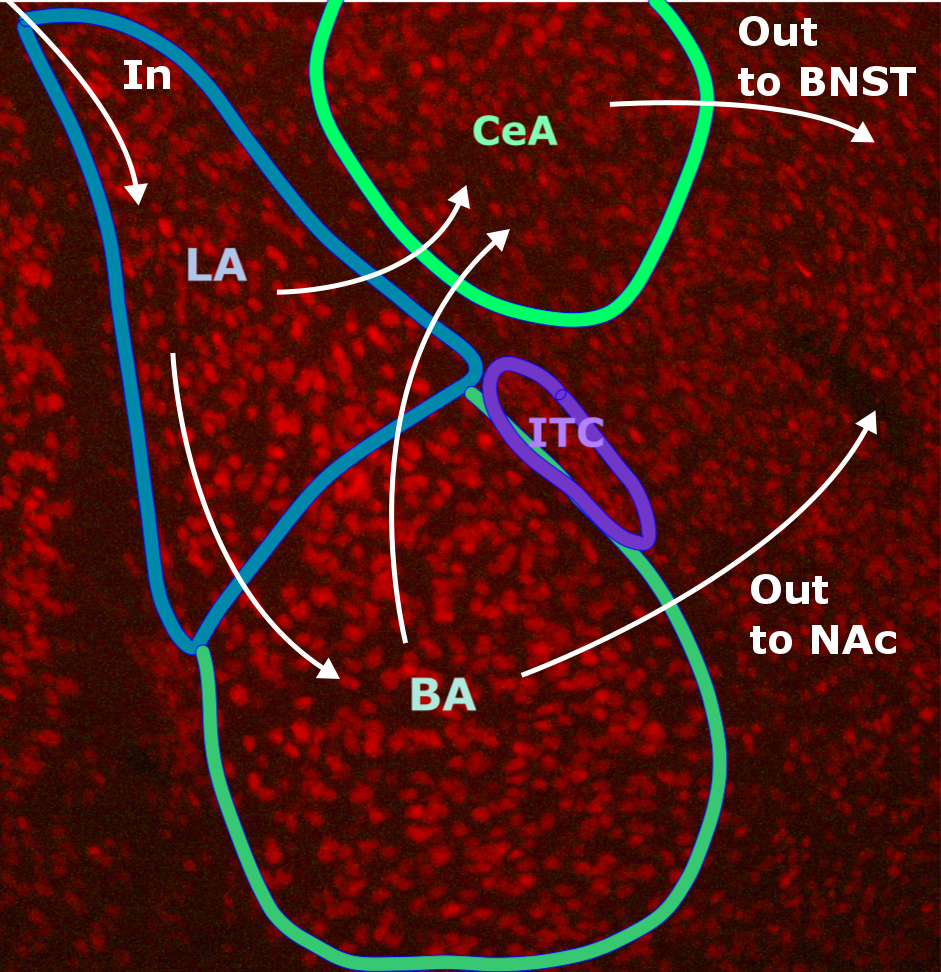
\includegraphics{source/figures/amygdaloidcomplex.jpg}
\caption{\textbf{Major nuclei of the amygdala.} The amygdaloid complex
with the major subnuclei and patterns of connectivity labeled. During
memory recall, sensory input is received by the LA, which sends
excitatory projections to both the BA and CeA. The BA, which also
receives input from the prefrontal cortex and hippocampus (not shown)
projects to the CeA in the case of fearful associations, or to the NAc
for rewarding associations. The CeA drives fear and anxiety related
behaviour through its connection with the BNST. ITC clusters situated
between the major subnuclei regulate the flow of information through the
circuit \label{ref_a_figure}}
\end{figure}

\subsection{The lateral amygdala}\label{the-lateral-amygdala}

The horn-shaped lateral amygdala is the most dorsally-situated nucleus
of the amygdala and is bordered ventrally by the basal nucleus,
laterally by the external capsule, and medially by the central nucleus.
The LA receives the majority of the sensory projections sent to the
amygdala and is thought to function as the amygdala's sensory interface
(LeDoux, Cicchetti, Xagoraris, \& Romanski, 1990). Somatosensory,
gustatory, auditory, and visual cortices all send heavy projections to
the LA, as do regions of the thalamus that carry corresponding
information. During auditory fear conditioning, auditory information
reaches the LA through both associative auditory areas and the medial
geniculate nucleus (MGN) of the thalamus. These two input streams are
thought to represent two distinct pathways of information: one carrying
complex, slow information from the cortex and one carrying early, but
simpler signals from the thalamus (Bergstrom \& Johnson, 2014). This
pattern is similar for visual information, with both cortical and
thalamic sources of information synapsing in the LA (C. Shi \& Davis,
2001). The LA also receives minor innervation from the prefrontal cortex
and hippocampal formation (entorhinal cortex and subiculum).

The LA projects to most other regions of the amygdaloid complex,
including the basal nucleus, central nucleus, and intercalated cell
regions. Interestingly, all of these regions send moderate to heavy
input back to the LA, suggesting that most of these connections are
reciprocal (Pitkanen, 2000). The purpose that this reciprocal
connectivity with the other subnuclei of the amygdala is unknown

The majority of neurons in the LA (\textasciitilde{}70\%) are
cortex-like, spiny pyramidal neurons similar to those found in
hippocampus or cortex. However, unlike in those regions, these neurons
are randomly organized without any parallel organization in any plane
and are naturally quiescent (P. Sah et al., 2003). The remaining neurons
primarily consists of a heterogenous population of non-pyramidal local
circuit interneurons that provide local inhibition through GABAergic
synapses (Spampanato, Polepalli, \& Sah, 2011).

\subsection{Subnuclei of the lateral
amygdala}\label{subnuclei-of-the-lateral-amygdala}

Although many studies have investigated the nuclei of the amygdala as if
they were uniform entities, classic tracing and electrophysiology
studies have identified important differences between small subregions,
including the LA (P. Sah et al., 2003). The LA has been proposed to
consist of three distinct subnuclei: dorsal, ventral-lateral, and
ventral-medial. These regions display different patterns of connectivity
to targets both within and outside the amygdala. However, how these
differences affect information processing during the formation and
retrieval of memories is largely unknown and unexplored.

The dorsal subnucleus of the lateral amygdala (LAd), situated at the tip
of the LA's horn-like structure receives the majority of the LA's
thalamic sensory inputs as well as containing the greatest degree of
overlap between auditory and somatosensory innervation (Asla Pitkänen,
Savander, Nurminen, \& Ylinen, 2003, Romanski et al. (1993)). The LAd
also receives the least amount of reciprocal projections from other
nuclei of the amygdala. One study using single-unit recording to measure
the activity of single neurons in the LA reported that neurons in the
LAd demonstrate the earliest changes in responsiveness to stimuli during
fear conditioning (Repa et al., 2001). These early-responding neurons
underwent rapid, but transient potentiation during fear learning that
decayed as memories became more stable over a number of training events,
a finding that was replicated in computational models (Dongbeom Kim,
Paré, \& Nair, 2013a). These observations lead the authors to propose
that these LAd neurons may be involved in a process of amygdalar memory
consolidation dependent on the LAd. However, empirical research since
this discovery has failed to replicate or expand upon these findings.

The other two subnuclei of the LA, the ventral-lateral (LAvl) and
ventral-medial (LAvm) also receive sensory input, but are distinguished
from the LAd by differences in the source of these inputs and in their
connectivity to other regions of the amygdala. The LAvl and LAvm both
receive local input from the LAd, but do not innervate each other,
suggesting that information flows unidirectionally through the LA (A.
Pitkänen, Savander, \& LeDoux, 1997). These subnuclei also receive the
majority of the reciprocal connections returned to the LA from the BA
and CeA. Generally, the sensory input that the LAvl and LAvm receive is
more cortical than thalamic in origin. In particular, the LAvm receives
most of its input from regions related to higher-order processing, such
as the prefrontal and perirhinal cortex and the hippocampus (A. Pitkänen
et al., 1997).

Despite the differences that have been demonstrated between these
subnuclei, it is difficult to draw conclusions as to how they interact
and contribute to memory function. For example, some inputs, such as
from the dorsal perirhinal cortex, have very little selectivity (C. J.
Shi \& Cassell, 1999). Furthermore, the high degree of connectivity
between these regions suggests that, even if sensory input is initially
received by a non-overlapping populations of neurons, it may later be
integrated through pathways that link these subnuclei.

\subsection{The basal amygdala}\label{the-basal-amygdala}

The basal nucleus of the amygdala is located ventrally to the LA and is
thought to integrate input from the LA related to sensory stimuli with
information related to context and cognitive processes. Similar to the
LA, the BA can be subdivided into distinct subregions: the
rostrocellular, magnocellular, and intermediate subnuclei (P. Sah et
al., 2003). The BA is highly connected with hippocampal and prefrontal
areas (Amano, Duvarci, Popa, \& Paré, 2011). In addition, the BA
contains the majority of the amygdala's projections to the nucleus
accumbens that mediate the expression of rewarding memories (Beyeler et
al., 2016).

Within the amygdaloid complex, the BA receives many large projections
from the LA and sends inputs back to the LA and CeA. The BA also
receives projections from thalamic and cortical sensory areas, but the
majority of its extra-amygdalar inputs come from the prefrontal cortex
and hippocampus, which are thought to contribute to the basal nucleus'
role in mediating the extinction and context dependency of learned
associations (Herry et al., 2008).

The BA contains a similar variety of neurons as the LA as distinguished
by morphology. However, neurons in the BA have been shown to have a
significantly higher baseline rate of firing than the LA (P. Sah et al.,
2003).

\subsection{The central amygdala}\label{the-central-amygdala}

The central nucleus of the amygdala is located in the dorsomedial region
of the amygdaloid complex and consists of two distinct subdivisions,
lateral and medial. These subdivisions engage in a great deal of
interplay during memory formation and retrieval, with the lateral
subdivision receiving the majority of the inputs from the LA and BA and
regulating the activity of the medial subdivision (Ehrlich et al.,
2009). The CeA is thought to function as the output center of the amygda
for fear and anxiety-related behaviour. During retrieval of a fear
memory, connections from the medial subdivision of the central amygdala
activate the nearby bed nucleus of stria terminalis (BNST), which then
activates downstream arousal and anxiety-producing regions of the
hypothalamus (S.-Y. Kim et al., 2013).

The morphological organization of the CeA is very different from that of
the other amygdaloid nuclei. This is likely due to their different
embryological origins, with the CeA sharing its developmental origin
with the primarily inhibitory striatum and the LA and BA developing
alongside excitatory, cortical regions (P. Sah et al., 2003). Unlike the
LA and BA, the CeA is primarily inhibitory and GABAergic, with abundant
local connections between subdivisions and a wide variety of
interneurons, some of which have been shown to play distinct roles in
anxiety (Botta et al., 2015).

\subsection{Intercalated cell regions}\label{intercalated-cell-regions}

The intercalated cell masses are groups of specialized GABAergic
interneurons located in between the lateral and basal nuclei and the
central nucleus. Although not much is known about these intercalated
cells, they have been shown to provide both feed-forward and feed-back
inhibition to the other nuclei of the amygdala and are thought to
function as an inhibitory gate that regulates the flow of information
between the input and output interfaces of the amygdala (Pape, 2005).

\section{Inhibitory Interneurons}\label{inhibitory-interneurons}

The amygdala, much like any other brain region, is highly dependent on
an appropriate balance between inhibitory and excitatory neural
activity. Throughout the amygdaloid complex, there is a wide variety of
inhibitory interneurons with various physiological properties and
patterns of connectivity (Ehrlich et al., 2009, P. Sah et al. (2003),
Spampanato et al. (2011), Waclaw, Ehrman, Pierani, \& Campbell (2010)).
In the LA and BA, these interneurons comprise about 20\% of the neuronal
population and have been shown to be central to the process of fear
conditioning (Ehrlich et al., 2009), coordinating the flow of
information between nuclei and gating sensory input through finely-tuned
systems of inhibition and disinhibition (Wolff et al., 2014). These
interneurons can be distinguished on the basis of the presence of
different molecular markers, including parvalbumin (PV), somatostatin
(SOM) and cholecystokinin (CCK), which are strongly correlated with
different functional characteristics.

\subsection{Parvalbumin-containing
Interneurons}\label{parvalbumin-containing-interneurons}

Interneurons that express the calcium-binding protein parvalbumin are
prevalent (\textasciitilde{}15\% of neurons) in the lateral and basal
nucleus of both the rodent and human amygdala (Sorvari, Miettinen,
Soininen, \& Pitkänen, 1996). PV\textsuperscript{+} cells display a
heterogeneity of firing properties (D. G. Rainnie, Mania, Mascagni, \&
McDonald, 2006), but generally share the same morphological
characteristics. PV\textsuperscript{+} interneurons almost always form
synapses on the cell bodies of principal neurons, where they are able to
effectively modulate neural excitability and mediate synchronous
oscillations (Freund \& Katona, 2007). PV\textsuperscript{+}
interneurons primarily receive input from local excitatory neurons.
However, they have been shown to be highly sensitive to sensory input
from both thalamus and cortex, suggesting that they may receive cortical
or thalamic innervation as well (Szinyei, Heinbockel, Montagne, \& Pape,
2000, Woodson, Farb, \& Ledoux (2000)).

\subsection{Somatostatin-containing
Interneurons}\label{somatostatin-containing-interneurons}

Somatostatin-containing interneurons represent a similar proportion of
the interneuronal population as those expressing PV (Sosulina,
Graebenitz, \& Pape, 2010). SOM\textsuperscript{+} interneurons display
a distinct delayed, stuttering pattern of firing in response to
stimulation. Importantly, SOM\textsuperscript{+} neurons form synapses
on the distal dendrites of pyramidal neurons rather than on the cell
body, which lends them the ability to selectively inhibit input arriving
on individual dendritic branches rather than manipulate whole-cell
excitability.

As the dominant interneuronal subtypes in the amygdala and hippocampus,
SOM\textsuperscript{+} and PV\textsuperscript{+} interneurons interact
with each other to a large extent. It has been suggested that
PV\textsuperscript{+} interneuron-mediated inhibition of
SOM\textsuperscript{+} cells gives rise to a process of disinhibitory
sensory control that is involved in the formation of associative
memories in both the hippocampus (Lovett-Barron et al., 2012) and LA
(Wolff et al., 2014). In both these regions, early activation of
PV\textsuperscript{+} interneurons has been proposed to inhibit
downstream SOM\textsuperscript{+} interneurons, thereby enhancing
responsiveness to sensory information delivered to the distal dendrites
of pyramidal neurons and promoting the excitability necessary for
plasticity and allocation to the engram.

\subsection{Cholecystokinin-containing
interneurons}\label{cholecystokinin-containing-interneurons}

Interneurons in the LA that express cholecystokinin are perhaps the most
diverse in terms of their functional properties (Jasnow, Ressler,
Hammack, Chhatwal, \& Rainnie, 2009). For example, they have been shown
to demonstrate both adapting and non-adapting firing, high and low input
resistance, as well as both fast and slow after-hyperpolarization
periods. This variety may be related to the fact that mRNA for CCK is
more broadly distributed throughout the region than any other molecular
marker used to distinguish interneuronal subtypes. In the amygdala, not
much is known about the functional role of CCK\textsuperscript{+}
interneurons. However, there has been some suggestion that a distinct
subtype of CCK\textsuperscript{+} cells may be specifically involved in
mediating anxiety related behaviour (Truitt, Johnson, Dietrich, Fitz, \&
Shekhar, 2009) .

\section{Modeling memory}\label{modeling-memory}

In order to understand a system as complex as the brain, it is necessary
to develop models that present simplified versions of phenomena. By
reducing the amount of variables in a model to those that are
specifically relevant to the function or task at hand it becomes much
easier to examine the relationship between relevant factors and test the
predictive or explanatory value of theories about how a system works.
Such models can be especially useful especially useful when they create
novel predictions that can then be tested experimentally. Since the time
of Donald Hebb, theoretical models in the field of learning and memory
have proven their usefulness for understanding how changes in the brain
give rise to memory.

Most computational models used to study learning and memory belong to a
class of models known as `neural networks'. These networks are based off
of nodes, simplified mathematical abstractions of neurons that are
connected to each other through connections (often referred to as edges)
that represent simplified synapses. Each node in a neural network has an
activation level that is determined by the input into that node from
outside the network, or from other nodes in the network. A node's
activation level can be thought of as the likelihood that it will
generate an output of its own or, alternatively, how active a neuron is
on a scale from 0 (not active) to 10 (fully active). The edges in the
neural network transmit this activation level between nodes, with the
amount of activity that is sent from the output node to the input node
determined by that edge's synaptic weight. Importantly, weights can have
both positive and negative values, corresponding to excitatory and
inhibitory connections in the brain (although some models allow nodes to
have output edges with both positive and negative weights, which is
biologically inaccurate). Each set of nodes that sends output to another
set of nodes is referred to as a layer. The result of this simple
architecture is that each node is capable of computing a weighted sum
from a number of inputs. Although this low-level operation is very
limited on its own, as more nodes (and layers of nodes) are added to a
neural network, and as rules are implemented that allow the connections
between nodes to be modified, their computational power becomes
increasingly powerful. In addition to being able to solve
computationally `hard' problems such as mastering the game of Go (Silver
et al., 2016), Neural networks have been used to successfully model many
forms of learning and memory, from Pavlovian conditioning (M. S.
Fanselow, 1998) to systems-level consolidation of long-term episodic
memories (Santoro, 2015).

\subsection{Autoassociative neural
networks}\label{autoassociative-neural-networks}

Hebb's original prediction for how memories could be stored in the brain
involved the simple rule that if cell A connects to a second cell B, and
if the two cells are repeatedly active at the same time, then the
connection between them is strengthened, so future activity in A is more
likely to activation in B (Hebb, 1949). This rule, now known as Hebbian
learning can be clearly replicated in neural networks in which the
strength of connections between nodes is increased if they are active at
the same time.

One class of neural network that implements Hebbian learning are
autoassociative netoworks. The distinguishing characteristic of these
networks is that each node is both an input and an output node, meaning
that it both receives input from external sources and contributes to the
overall output of the nework by transmitting its activity to other nodes
(Gluck \& Myers, 2001). When a pattern of input activates an
autoassociative network, some subset of nodes are activated by that
external input, while others remain silent. Which neurons are activated
is determined both by the connectivity and weights of external inputs
and, because nodes are able to excite each other, pre-existing weights
between nodes in the network (Figure 1.2a). If a novel pattern of
external input is received, Hebbian learning in the autoassociative
network ensures that the synaptic weights of edges between coactive
nodes are strengthened such that the subset of neurons activated by
external input are bound together into an ensemble, storing this pattern
in the network (Figure 1.2b,c). Later, if an incomplete or distorted
version of the same input is given to the network, this pattern is more
likely to be reinstated due to the enhanced connectivity between those
neurons that were most excited by the original input. This process,
known as pattern completion, is thought to play an important role in the
brains' ability to recognize patterns in our environment and recall
previous sensory representations during classical conditioning (ie. if a
tone and shock are presented simultaneously, nodes that respond
selectively to either stimulus will be linked such that later
presentation of either tone or shock alone will lead reactivation to the
entire population that was active when both tone and shock were
presented).

\begin{figure}[htbp]
\centering
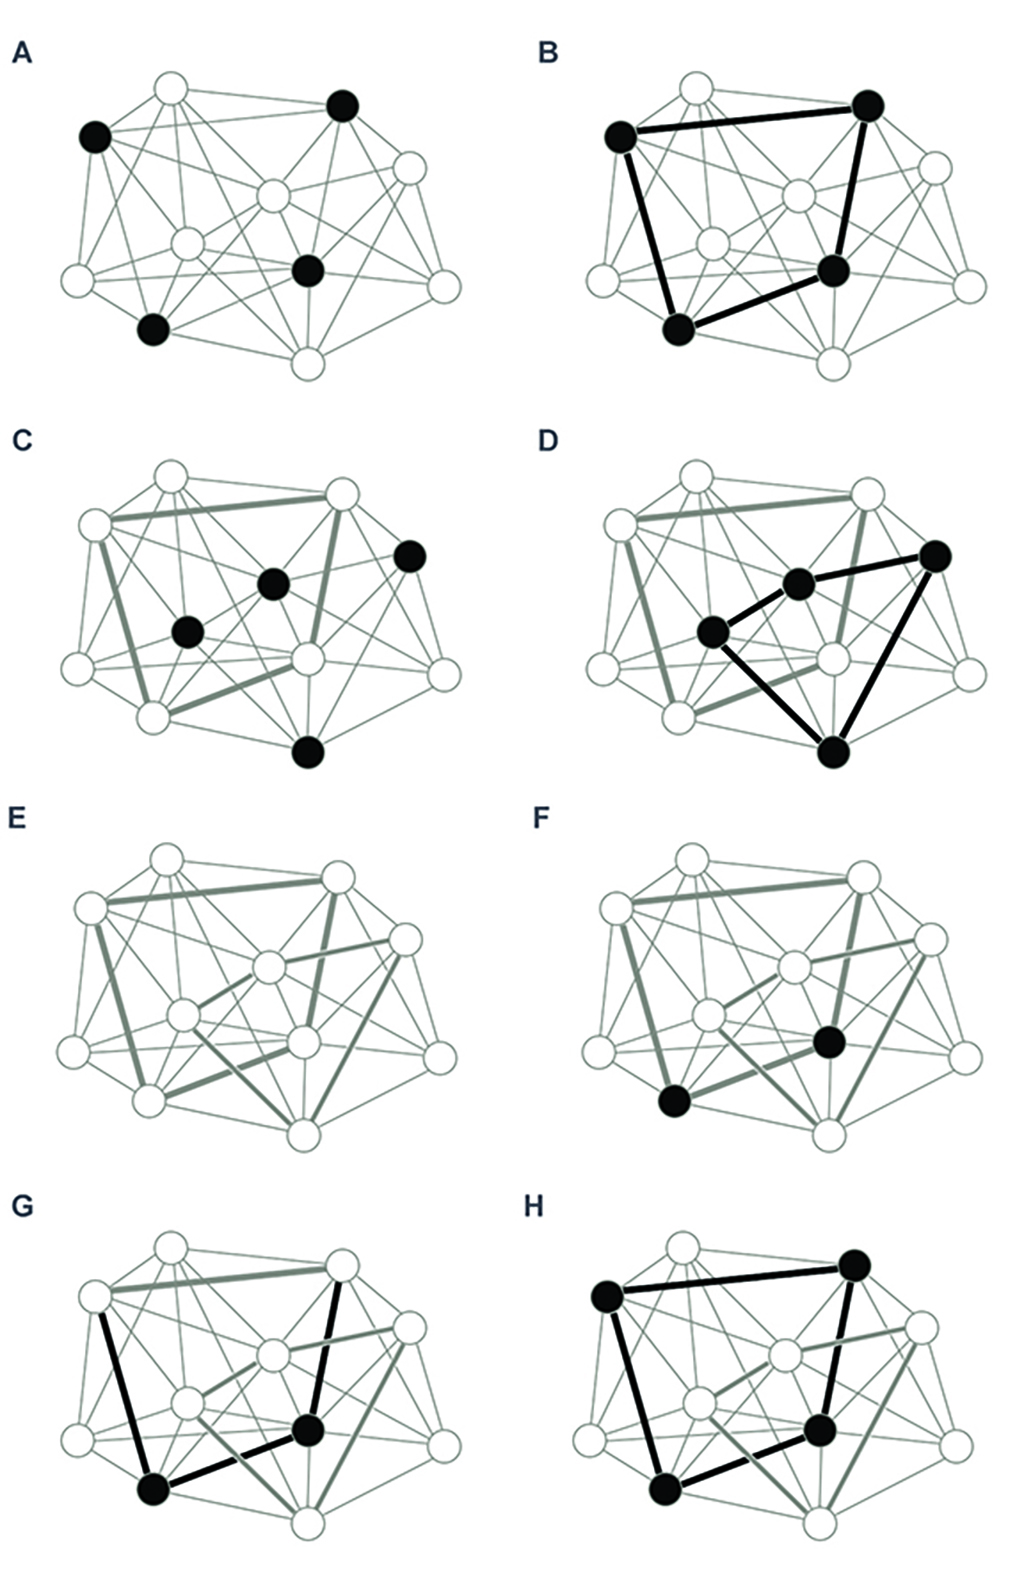
\includegraphics{source/figures/autoassociative.jpg}
\caption{\textbf{Autoassociative memory.} Illustration of
autoassociative memory encoding and retrieval. (A) Sensory input (not
shown) to the network activates a certain subset of nodes (solid
circles). (B) Hebbian learning leads to the strengthening of the
weightened connections between nodes that are activated by sensory
input, storing this pattern of activity. (C) Later, a different new
pattern of sensory stimuli evokes the activation of a different subset
of nodes in the network. (D) Weights between nodes active during this
new pattern are strengthened and (E) both patterns are now stored in the
network (heavy lines). (F) If a partial version of a previously stored
pattern is presented to the netowork, some of the nodes involved in that
pattern will be activated. (G) Activation will then flow along
previously strengthened connections and lead to (H) the reactivation of
the previously stored pattern. Adapted from Gluck and Myers, 2001.
\label{ref_a_figure}}
\end{figure}

\subsection{Sparse distributed memory}\label{sparse-distributed-memory}

The theory of sparse distributed memory is a mathematical model that
attempts to describe how memory could be implemented in the brain with a
formal, quantified approach. Sparse distributed memory does not require
neural networks (indeed, it has been widely implemented in the world of
traditional computer science), but it is very easily implemented by
neural networks, including autoassociative networks. The central
principle of sparse distributed memory is the statistical recall of
previously active patterns distributed across a range of different
locations in a very large network (Kanerva, 1988).

In order to understand sparse distributed representations, it is best to
draw comparisons with other coding schemes such as local coding. In a
local coding, every unit of information is stored at a single location
with no overlap between units. A common analogy to this is a computer
keyboard, where each key matches to a character in a one-to-one fashion.
In neuroscience, local coding is expressed to the extreme by ``Brad Pitt
neuron'' hypothesis. In this hypothesis, there exist neurons that store
memories for only one particular person, place, or thing. When, for
example, an image of Brad Pitt is shown, the recognition of Brad Pitt is
mediated entirely by the firing of a single ``Brad Pitt neuron''. Local
representations have the advantage of being easy to decode (the memory
is always in one location) and they avoid the risk of interference
between memories. However, they have extremely low capacity, as every
memory requires its own dedicated location, and they are inflexible, as
new memory addresses would need to be added to permit new learning.
Furthermore, because memories are disconnected from each other, such
representations do not allow memories to be linked or generalized in any
way. This lack of flexibility would be completely untenable for an
organism required to navigate a noisy world of fuzzy inputs.

Another example of a coding scheme that is inefficient within in the
hardware of the brain is dense coding. This is the form of memory
implemented by computer binary that stores information as patterns
distributed across the entirety of a fixed number of locations. For
example, in ASCII code, each letter is encoded as a string of 8 binary
values. When this string is read, the computer then reads each bit and
performs a lookup operation to determine which character corresponds to
the string that has been read (01100001 = a, 01100010 =b, etc.). Such a
coding scheme is convenient for use in computers because only a small
number of bits need to be read to encode a large number of distinct
memories (8 bits = 256 possible combinations). However, there are
significant drawbacks to this scheme outside of the orderly, immutable
world of computer memory. First, because all possible locations (bits)
must be read in order to perform the lookup operation, only one pattern
can be present in the network at one time. Furthermore, dense
representations are very sensitive to noise. Each pattern of active
locations represents a distinct memory, so if one the activity of one
location is altered, the memory that is retrieved will be completely
changed.

The substrate of the brain is very different from a computer: cells and
synapses are constantly being modified or turned over, and the input
cues that networks receive during memory retrieval are noisy. In this
environment, the most effective coding scheme is sparse distributed
memory, where information is spread across a sparse subset of units in a
larger total population. At their most basic form, sparse distributed
memory networks can be represented as very large sets of locations, with
only a small percentage of those locations active during the
representation of any one piece of information. Because there is so much
`room' in the set of locations, sparse codes can coexist in the same
network. Furthermore, each individual location can be involved in the
representation of multiple memories. Overlap between patterns can be
used to encode associations between memories. Additionally, memories can
be recalled from incomplete or corrupted input patterns as presenting
the network with partial pattern is able to narrow the range of
appropriate stored patterns to practical degrees of statistical
certainty (Ahmad \& Hawkins, 2015). Sparse distributed representations
also allow new patterns to be stored simply by altering the connectivity
of existing units, such as in a neural network. No new addresses need to
be created to store new patterns. Rather, the network merely needs to be
modified enough to create a new pattern of activity that is sufficiently
different from pre-existing patterns. These features, along with
neurophysiological data showing sparse patterns of activity during
memory retrieval in the amygdala (Bach, Weiskopf, \& Dolan, 2011)
hippocampus (Wixted et al., 2014) provide strong evidence for the use of
sparse coding in the brain.

\subsection{Modeling memory allocation in the lateral
amygdala}\label{modeling-memory-allocation-in-the-lateral-amygdala}

In order to understand the mechanisms contributing to the induction and
storage of emotional memories, a significant amount of work has been
done to develop neural network models of the LA. One such model,
introduced by D. Kim, Paré, \& Nair, consists of an autoassociate neural
network that contains both excitatory and inhibitory cells, implements
Hebbian forms of long-term potentiation and depression, and replicates
patterns of intra-LA connectivity discovered by systematic
electrophysiological recording studies in the rat LA. By delivering
input to the network corresponding to what would occur during auditory
fear conditioning, the group has been able to replicate the findings of
several electrophysiological and IEG-based studies and has gone on to
make proposals about the mechanisms by which neurons are allocated to
the engram during encoding.

A series of experimental work in mice has demonstrated that neuronal
excitability plays a central role in biasing allocation to an engram
(Han et al., 2007, Hsiang et al. (2014), Yiu et al. (2014), Y. Zhou et
al. (2009)). However, artificially increased excitability of up to 20\%
of LA neurons in these studies did not increase the overall size of the
of the LA component of the engram (in terms of number of neurons),
suggesting that allocation is a competitive process. However, these
studies were unable to explain how this process of competition occurs or
what purpose it serves. In order to answer these questions, Kim et al.
performed a series of experiments in their model, arbitrarily increasing
the excitability of subsets of excitatory neurons and recording the
effects on the size of the stable engram after repeated training in an
auditory fear conditioning paradigm. Interestingly, they were able to
replicate and extend the effect demonstrated in previous studies:
increasing excitability in up to 25\% of cells did not alter the size of
the memory trace (Dongbeom Kim, Paré, \& Nair, 2013c). Furthermore, with
the control their model afforded them, they were able to demonstrate
that inhibition is the primary factor in constraining neuronal
allocation to an engram (Feng, Samarth, Paré, \& Nair, 2016). Their
model demonstrates that competitive interactions between principal
neurons are mediated by disynaptic connections involving inhibitory
interneurons. Essentially, highly excitable principal neurons activated
during learning inhibit many of their principal neuron neighbors via
indirect, inhibitory connections. Highly excitable principal neurons
that share excitatory connections with each other become even more
excited, while principal neurons that primarily receive disynaptic
inhibitory connections from this highly excitable subset are silenced.
This process magnifies the difference in excitability between `winners'
and `loser' neurons. Furthermore, they demonstrate that plasticity at
inhibitory synapses is able to compensate for increases in excitability
such as would be seen during CREB overexpression.

This neural network modelling approach was also able to suggest why
engrams in the LA are constrained. First, the sparse code enforced by
competitive interactions is consistent with theoretical models of sparse
distributed coding schemes that have also been demonstrated in other
areas of the brain, such as hippocampus (Wixted et al., 2014) and cortex
(Gdalyahu et al., 2012) Thus, it reasonable to assume that the LA
benefits from the many advantages of sparse distributed representations
in a neural substrate (high capacity, robustness to noise). Second, the
model revealed that sparsity enforced by competitive interactions could
ensure an optimal degree of stimulus specificity (D. Kim, Samarth, Feng,
Pare, \& Nair, 2015). By selectively modulating plasticity of either
excitatory or inhibitory synapses, the researchers demonstrated that
excitatory connectivity drives the number of cells allocated to the
engram upwards, but increases the probability that memories will be
generalized. Inhibitory connectivity had the opposite effect, decreasing
the proportion of engram cells and making memories more specific. For an
animal in the wild, the balance between memory specificity and
generalizability is extremely important, drawing the line between
failure to respond to threats and chronic anxiety.

\chapter*{List of tables}\label{list-of-tables}
\addcontentsline{toc}{chapter}{List of tables}

Table 5.1 This is an example table . . . \hfill{pp}\\
Table x.x Short title of the figure . . . \hfill{pp}

\chapter{Introduction, with a
citation}\label{introduction-with-a-citation}

\section{Background}\label{background}

This is the introduction. Quisque finibus aliquet cursus. Integer in
pellentesque tellus. Duis eu dignissim nulla, a porttitor enim. Quisque
vehicula leo non ultrices finibus. Duis vehicula quis sem sit amet
sollicitudin. Integer neque est, pharetra et auctor vel, iaculis
interdum lectus.

To include a citation to the text, just add the citation key shown in
the references.bib file. The style of the citation is determined by the
ref\_format.csl file. For example, in The Living Sea you can find
pictures of the Calypso ({\textbf{???}}).

In neque mauris, maximus at sapien a, iaculis dignissim justo. Aliquam
erat volutpat. Praesent varius risus auctor est ultricies, sit amet
consequat nisi laoreet. Suspendisse non est et mauris pharetra sagittis
non porta justo. Praesent malesuada metus ut sapien sodales ornare.

\section{The middle bit}\label{the-middle-bit}

This is the middle bit. Phasellus quis ex in ipsum pellentesque lobortis
tincidunt sed massa. Nullam euismod sem quis dictum condimentum.
Suspendisse risus metus, elementum eu congue quis, viverra ac metus.
Donec non lectus at lectus euismod laoreet pharetra semper dui. Donec
sed eleifend erat, vel ultrices nibh. Nam scelerisque turpis ac nunc
mollis, et rutrum nisl luctus.

Duis faucibus vestibulum elit, sit amet lobortis libero. Class aptent
taciti sociosqu ad litora torquent per conubia nostra, per inceptos
himenaeos. Sed at cursus nibh. Sed accumsan imperdiet interdum. Proin id
facilisis tortor. Proin posuere a neque nec iaculis. Suspendisse
potenti. Nullam hendrerit ante mi, vitae iaculis dui laoreet eu.

Cras eleifend velit diam, eu viverra mi volutpat ut. Cum sociis natoque
penatibus et magnis dis parturient montes, nascetur ridiculus mus. Donec
finibus leo nec dui imperdiet, tincidunt ornare orci venenatis. Maecenas
placerat efficitur est, eu blandit magna hendrerit eu.

\subsection{Subsection of the middle
bit}\label{subsection-of-the-middle-bit}

This is a subsection of the middle bit. Quisque sit amet tempus arcu, ac
suscipit ante. Cras massa elit, pellentesque eget nisl ut, malesuada
rutrum risus. Nunc in venenatis mi. Curabitur sit amet suscipit eros,
non tincidunt nibh. Phasellus lorem lectus, iaculis non luctus eget,
tempus non risus. Suspendisse ut felis mi.

\section{Summary of chapters}\label{summary-of-chapters}

This is a brief outline of what went into each chapter. \textbf{Chapter
1} gives a background on duis tempus justo quis arcu consectetur
sollicitudin. \textbf{Chapter 2} discusses morbi sollicitudin gravida
tellus in maximus. \textbf{Chapter 3} discusses vestibulum eleifend
turpis id turpis sollicitudin aliquet. \textbf{Chapter 4} shows how
phasellus gravida non ex id aliquet. Proin faucibus nibh sit amet augue
blandit varius.

\chapter{Methods}\label{methods}

\section{Mice}\label{mice}

Except where noted, adult (at least 8 weeks of age) male and female F1
hybrid (C57BL/6NTac X 129S6/SvEvTac) wild-type (WT) mice were used in
all experiments. Mice were bred at the Hospital for Sick Children,
provided with food and water ad libitum, and group housed (4 per cage)
on a 12 h light/dark cycle. All mice were briefly single housed,
transported, and handled once daily for 6 days prior to experiments. All
experiments were performed during light-phase. All procedures were
conducted in accordance with policies of the Hospital for Sick Children
Animal Care and Use Committee and conformed to both Canadian Council on
Animal Care (CCAC) and National Institutes of Health (NIH) Guidelines on
Care and Use of Laboratory Animals. For experiments involving
PV\textsuperscript{+} interneuron inhibition, heterozygous PV-Cre
knockin driver mice (B6;129P2-Pvalbtm1(cre)Arbr/J) maintained on a
C57BL/6 genetic background were used. These mice express Cre recombinase
in PV neurons, without disrupting endogenous PV expression. PV-Cre mice
were obtained from Jackson Labs and were originally generated by Silvia
Arber, FMI (Hippenmeyer et al., 2005).

\section{Auditory Fear Conditioning}\label{auditory-fear-conditioning}

Auditory fear training involved placing mice into a conditioning chamber
and, 2 minutes later, presenting a tone (2,800 Hz, 85 dB, 30 s) that
co-terminated with a 2s footshock. Testing was performed 24 hours later
by placing mice in a novel context and, after a 2 minute baseline
period, presenting an identical tone for 1 minute. During testing, an
overhead camera captured the animal's activity and was used to assess
percentage time spent freezing during the tone (defined as an
immobilized, crouched position with an absence of any movement except
respiration (M. S. Fanselow \& Bolles, 1979).

\section{Immunohistochemistry}\label{immunohistochemistry}

We used the expression of Arc protein in neurons active following
training or a memory test as a proxy for identifying neurons that
compose part of an engram supporting that memory. Arc protein is
reliably elevated in excitatory neurons 90 min after activity (John F.
Guzowski et al., 2005) and has been used as a proxy for visualizing
neuronal components of an engram (Gouty-Colomer et al., 2015). 90
minutes after the delivery of the tone during training or testing, mice
were transcardially perfused with 4\% paraformaldehyde (PFA) and brains
removed. Brains remained in PFA for 1 day and were then transferred into
cryoprotectant solution (20\% sucrose) at 4 ºC. Three days later, brains
were sectioned into 50 μm sections using a cryostat with an inter-slice
interval of 100 um. Slices were then washed and incubated overnight with
Arc polyclonal rabbit antibody (1:500, Synaptic Systems, Cat. No. 156
003) at 4 ºC . In the experiment involving manipulations of shock
intensity, slices were also incubated with NeuN polyclonal mouse
antibody (1:1000, Millipore, MAB377). Staining was visualized either
with 3,3′-Diaminobenzidine (DAB) or fluorescent secondary goat
anti-rabbit Alexa 288 (1:1000, Life Technologies, Cat. No. A11034) and
goat anti-mouse Alexa 568 (1:1000, Life Technologies, Cat. No. A11004)
antibodies. Measures of Arc\textsuperscript{+} cell density by area in
the first experiment using DAB were obtained by imaging sections under a
10x Nikon light microscope and manually counting the number of
Arc\textsuperscript{+} cells in these images with ImageJ software (NIH)
(Schneider et al., 2012) by experimenters blind to the treatment
condition. ANOVAs with post-hoc Fisher's LSD tests were conducted to
compare Arc\textsuperscript{+} cell density between different treatment
groups within each amygdala nucleus.

\section{AAV Vector}\label{aav-vector}

The AAV8-hSyn-DIO-hM4Di-mCherry vector was obtained from the UNC Vector
Core (Chapel Hill, NC). This adeno-associated virus (AAV) contains a
double floxed inverse open reading frame of hM4Di fused to mCherry that
is expressed from the human synapsin (hSyn) promoter after recombination
by Cre recombinase (Krashes et al., 2011). The average titer of the
virus stocks was 4.0 × 107 infectious units/ml. Mice were allowed to
recover for 4 weeks for maximal viral expression before performing
behavioural experiments.

\section{Surgery}\label{surgery}

Before surgery, mice were pre-treated with atropine sulfate (0.1 mg/kg,
ip), anesthetized with chloral hydrate (400 mg/kg, ip) and placed in a
stereotaxic frame. Skin was retracted and holes were drilled in the
skull above the amygdala (AP = -1.4 mm, ML = ±3.4 mm, V = -5.0 mm from
bregma). AAV-DIO-hM4Di-mCherry (1.0 μl) was infused bilaterally into the
amygdala. After surgery, mice recovered for 4 hours before being
returned to their standard housing.

\section{catFISH}\label{catfish}

Mice were trained with various shock conditions (1 x 0.4 mA, 1 x 0.7 mA,
and 3 x 0.7 mA) in order to create memories of different strengths. A
group that received a shock immediately upon entering the chamber was
included as a control. 5 minutes after either training or testing,
animals were sacrificed and brains were subsequently processed with
catFISH. Brains were then imaged and analyzed with systematic
stereological procedures to identify the proportion of
\emph{Arc\textsuperscript{+}} neurons in the LA. We performed catFISH
for \emph{Arc} mRNA to identify neurons activated during fear
conditioning or retrieval. 5 min after either auditory fear conditioning
or testing, brains were removed and frozen. Tissue was then sectioned
(20 m) and prepared for FISH according to previously described
protocols (Han et al., 2007). Visualization of \emph{Arc} mRNA was
performed through the use of a DIG-conjugated anti-sense probe
corresponding to the Arc open reading frame. In order to minimize
differences in staining, sections from 4 mice were mounted together on
one slide. After hybridization and amplification of \emph{Arc} and H1a
signals, counterstaining with Hoechst 33258 to visualize nuclei was
performed.

Following catFISH processing, sections were imaged on a laser confocal
microscope (Zeiss LSM 710) to obtain optical z-stack series with a step
size ≤ 1 m apart. Stacks were analyzed for nuclear \emph{Arc}
intranuclear fluorescence by two individuals unaware of treatment
condition. Stereological counting was then performed by two individuals
unaware of treatment condition, with at least four sections counted for
each mouse.

\section{Stereological Counting}\label{stereological-counting}

In order to accurately determine the proportion of neurons active in the
LA during auditory fear training and testing, we used unbiased
stereological principles and systematic sampling techniques to obtain
the ratio of Arc-expressing neurons to the number of total neurons. For
the experiment involving manipulation of shock intensity, it was
possible to use expression of the neuron-specific protein NeuN to obtain
a measure of the neuronal population directly. However, for experiments
involving AAV-DIO-hM4Di-mCherry, the nuclear stain
4',6-diamidino-2-phenylindole (DAPI) was used to obtain a measure of the
total cellular population that was later adjusted based on an
empirically determined estimate of the ratio of neurons to total cells
in the LA. Several sections containing both DAPI and NeuN were analyzed
to obtain this empirical estimate (78.9\% ± 2.355, n = 10).
Stereological counts were adjusted by this ratio without affecting the
relationships between groups.

Counting was performed by an experimenter blind to the treatment
condition using the Optical Fractionator probe within Stereo
Investigator (version 10, MBF Bioscience, Williston, VT USA). Counting
was performed on every third section (50 μm thickness, at least 5
sections per mouse) from the left hemisphere. A counting frame of 120 μm
x 120 μm was randomly distributed according to a 250 μm x 250 μm grid
throughout the LA. Section thickness was recorded at every sampling site
to compensate for any potential thickness variation across the sections
due to tissue processing. A 12 μm dissector height was used with 2 μm
guard zones placed at the top and bottom of each section. Coefficient of
Error values, determined by Gundersen's method (Gundersen \& Jensen,
1987) (m=1) were \textless{} 0.11 in all samples. For analysis of LA
subnuclei, contours were drawn between regions as defined by a
stereotaxic atlas (Paxinos \& Franklin, n.d.). All stereological data
was collected only from the left hemisphere in order to avoid potential
hemispheric differences in Arc activity, although preliminary results
showed no significant difference in Arc\textsuperscript{+} cell density
between hemispheres (paired t-test, P \textgreater{} 0.1).

\section{CNO}\label{cno}

CNO (Toronto Research Chemicals {[}TRC{]}) was prepared in a stock
solution of 10 mg/ml in DMSO and subsequently diluted to a working
concentration of 1 mg/ml in phosphate-buffered saline (PBS). CNO was
injected intraperitoneally at a dosage of 2.0 mg/kg 1hr before training.
Vehicle solution used as a control consisted solely of PBS.  

\chapter{Hypothesis}\label{hypothesis}

The goal of this thesis is two part. First, to provide evidence that the
lateral amygdala performs sparse coding, whereby memories are allocated
to similar proportions of neurons despite differences in the strength of
those memories. Second, to show that inhibitory interneurons are
implicated in the mechanisms that ensure this sparse coding. To test
these hypotheses, I will manipulate memory strength in an auditory fear
conditioning paradigm and measure the proportion of neurons in the LA
allocated to an engram of conditioned fear. I will then perform a
similar experiment including the inactivation a subset of inhibitory
PV\textsuperscript{+} interneurons in the LA during fear conditioning.
If these inhibitory cells are involved in a mechanism that constrains
the engram, I predict that this manipulation will alter the number of
the neurons allocated to the engram. Together, these results should
provide novel evidence for the existence of memory allocation mechanisms
in the LA that involve inhibitory interneurons.

\chapter{Literature review, with
maths}\label{literature-review-with-maths}

\section{Introduction}\label{introduction-1}

This is the introduction. Duis in neque felis. In hac habitasse platea
dictumst. Cras eget rutrum elit. Pellentesque tristique venenatis
pellentesque. Cras eu dignissim quam, vel sodales felis. Vestibulum
efficitur justo a nibh cursus eleifend. Integer ultrices lorem at nunc
efficitur lobortis.

\section{The middle}\label{the-middle}

This is the literature review. Nullam quam odio, volutpat ac ornare
quis, vestibulum nec nulla. Aenean nec dapibus in
mL/min\textsuperscript{-1}. Mathematical formula can be inserted using
Latex:

\begin{enumerate}
\def\labelenumi{(\arabic{enumi})}
\tightlist
\item
  \(f(x) = ax^3 + bx^2 + cx + d\)
\end{enumerate}

Nunc eleifend, ex a luctus porttitor, felis ex suscipit tellus, ut
sollicitudin sapien purus in libero. Nulla blandit eget urna vel tempus.
Praesent fringilla dui sapien, sit amet egestas leo sollicitudin at.

Pellentesque habitant morbi tristique senectus et netus et malesuada
fames ac turpis egestas. Sed faucibus pulvinar volutpat. Ut semper
fringilla erat non dapibus. Nunc vitae felis eget purus placerat finibus
laoreet ut nibh.

\section{Conclusion}\label{conclusion}

This is the conclusion. Donec pulvinar molestie urna eu faucibus. In
tristique ut neque vel eleifend. Morbi ut massa vitae diam gravida
iaculis. Pellentesque habitant morbi tristique senectus et netus et
malesuada fames ac turpis egestas.

\begin{itemize}
\tightlist
\item
  first item in the list
\item
  second item in the list
\item
  third item in the list
\end{itemize}

\chapter{First research study, with
code}\label{first-research-study-with-code}

\section{Introduction}\label{introduction-2}

This is the introduction. Nam mollis congue tortor, sit amet convallis
tortor mollis eget. Fusce viverra ut magna eu sagittis. Vestibulum at
ultrices sapien, at elementum urna. Nam a blandit leo, non lobortis
quam. Aliquam feugiat turpis vitae tincidunt ultricies. Mauris
ullamcorper pellentesque nisl, vel molestie lorem viverra at.

\section{Method}\label{method}

Suspendisse iaculis in lacus ut dignissim. Cras dignissim dictum
eleifend. Suspendisse potenti. Suspendisse et nisi suscipit, vestibulum
est at, maximus sapien. Sed ut diam tortor.

\subsection{Subsection 1 with example code
block}\label{subsection-1-with-example-code-block}

This is the first part of the methodology. Cras porta dui a dolor
tincidunt placerat. Cras scelerisque sem et malesuada vestibulum.
Vivamus faucibus ligula ac sodales consectetur. Aliquam vel tristique
nisl. Aliquam erat volutpat. Pellentesque iaculis enim sit amet posuere
facilisis. Integer egestas quam sit amet nunc maximus, id bibendum ex
blandit.

For syntax highlighting in code blocks, add three ```'' characters
before and after a code block:

\begin{Shaded}
\begin{Highlighting}[]
\NormalTok{mood }\OperatorTok{=} \StringTok{'happy'}
\ControlFlowTok{if} \NormalTok{mood }\OperatorTok{==} \StringTok{'happy'}\NormalTok{:}
    \BuiltInTok{print}\NormalTok{(}\StringTok{"I am a happy robot"}\NormalTok{)}
\end{Highlighting}
\end{Shaded}

\subsection{Subsection 2}\label{subsection-2}

This is the second part of the methodology. Proin tincidunt odio non sem
mollis tristique. Fusce pharetra accumsan volutpat. In nec mauris vel
orci rutrum dapibus nec ac nibh. Praesent malesuada sagittis nulla, eget
commodo mauris ultricies eget. Suspendisse iaculis finibus ligula.

\section{Results}\label{results}

These are the results. Ut accumsan tempus aliquam. Sed massa ex, egestas
non libero id, imperdiet scelerisque augue. Duis rutrum ultrices arcu et
ultricies. Proin vel elit eu magna mattis vehicula. Sed ex erat,
fringilla vel feugiat ut, fringilla non diam.

\section{Discussion}\label{discussion}

This is the discussion. Duis ultrices tempor sem vitae convallis.
Pellentesque lobortis risus ac nisi varius bibendum. Phasellus volutpat
aliquam varius. Mauris vitae neque quis libero volutpat finibus. Nunc
diam metus, imperdiet vitae leo sed, varius posuere orci.

\section{Conclusion}\label{conclusion-1}

This is the conclusion to the chapter. Praesent bibendum urna orci, a
venenatis tellus venenatis at. Etiam ornare, est sed lacinia elementum,
lectus diam tempor leo, sit amet elementum ex elit id ex. Ut ac viverra
turpis. Quisque in nisl auctor, ornare dui ac, consequat tellus.

\chapter{Results}\label{results-1}

\section{Arc expression increases in the amygdala after fear
conditioning}\label{arc-expression-increases-in-the-amygdala-after-fear-conditioning}

Similar to previous studies (Gouty-Colomer et al., 2015, Reijmers et al.
(2007), Tayler et al. (2013)), Arc protein expression was visualized 90
min after memory retrieval to identify neurons that were active during
memory encoding or retrieval as part of an engram. Specifically, mice
were trained in auditory fear conditioning and the number of neurons
positive for Arc (Arc\textsuperscript{+}) 90 min following various
manipulations (e.g., initial training or memory recall) was examined
(Figure 1a). Arc\textsuperscript{+} neuron density (per 100 µm2) was
assessed in the LA, BA, central amygdala (CeA) and intercalated cell
masses (ITC) (Figure 4.1b). Non-learning control groups were also
included (homecage mice, mice exposed to tone alone, chamber alone or an
immediate shock) (Frankland et al., 2004, Zelikowsky, Hersman, Chawla,
Barnes, \& Fanselow (2014)).

There was a significant increase in the number of Arc\textsuperscript{+}
neurons throughout the amygdala after both training and testing (Figure
4.1c). Arc\textsuperscript{+} cell density was elevated both after
training and testing (in comparison to homecage controls) in the LA
{[}F(5, 36) = 10.63, P \textless{} 0.001{]}, BA {[}F(5, 36) = 5.20, P
\textless{} 0.001{]} and CeA {[}F(5, 36) = 4.99, P \textless{} 0.001{]}.
However, there was no significant difference in Arc\textsuperscript{+}
density between treatments in the ITC region {[}F(5, 36) = 1.86, P
\textgreater{} 0.05{]}. Importantly, the control tone alone, chamber
alone or immediate shock groups did not differ from the homecage group
in any amygdala region (P \textgreater{} 0.1). Fear training and testing
induced a similar number of Arc\textsuperscript{+} neurons in many
amygdala regions (LA, P \textgreater{} 0.5; BA, P \textgreater{} 0.1;
CeA, P \textgreater{} 0.5; ITC, P \textgreater{} 0.5), suggesting that a
similar number of neurons were active during encoding and retrieval of
an auditory fear memory.

\begin{figure}[htbp]
\centering
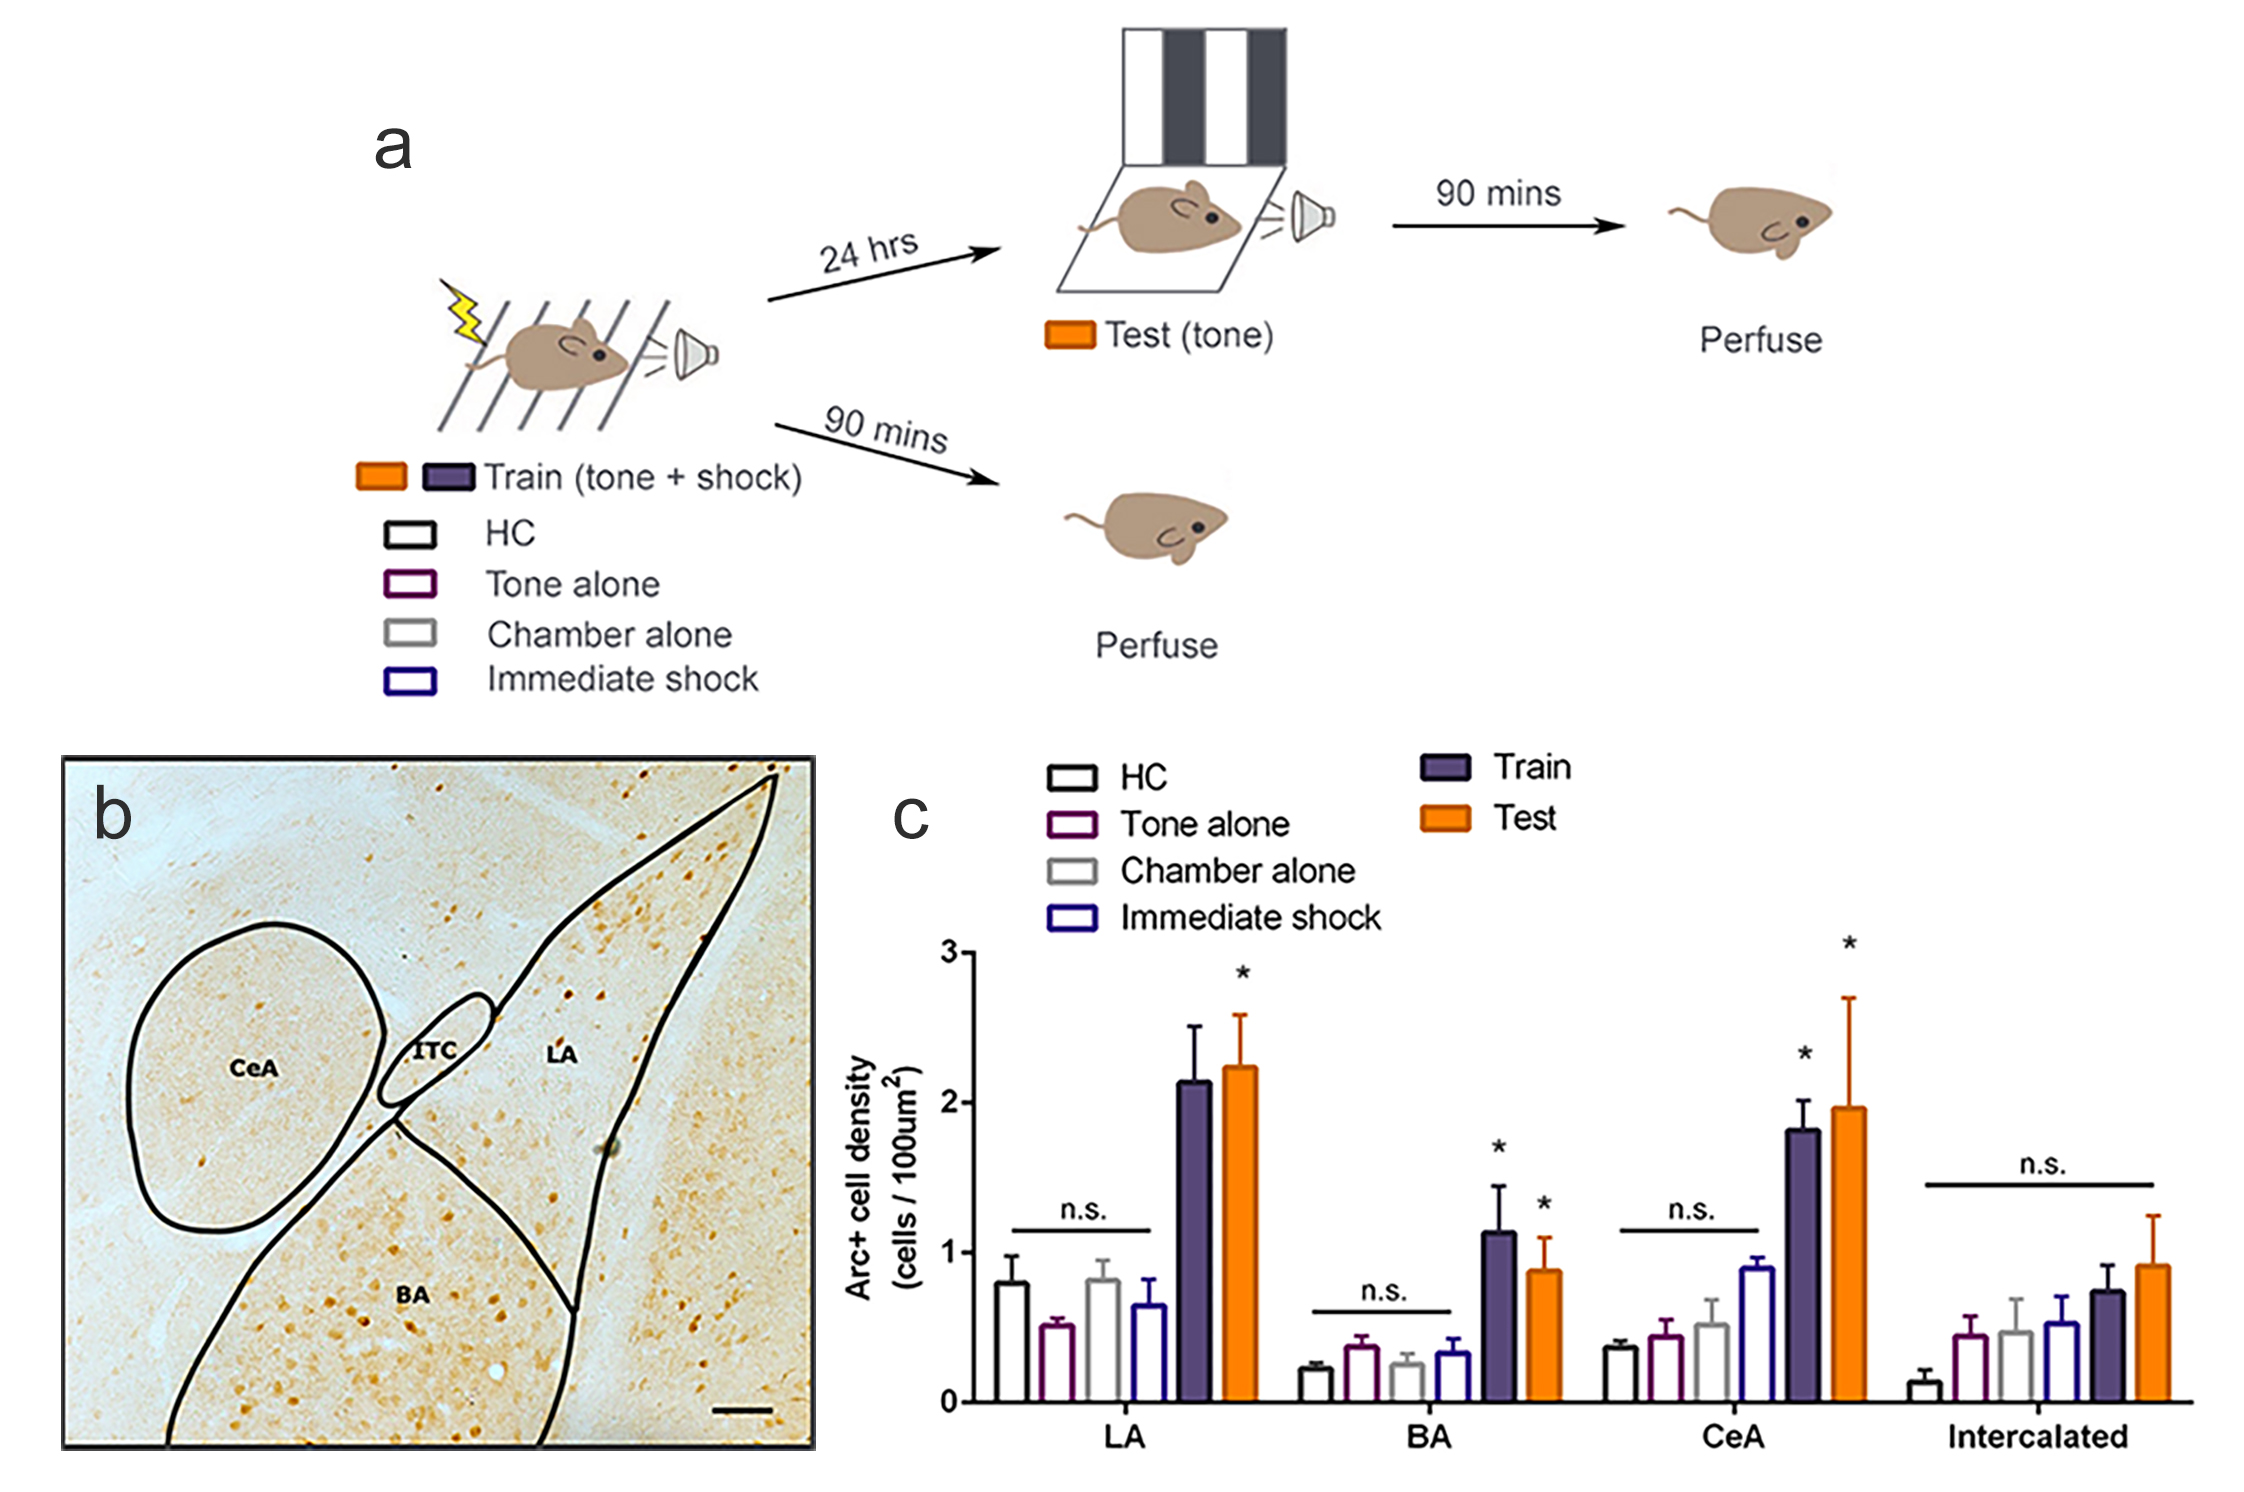
\includegraphics{source/figures/figure_1.jpg}
\caption{\textbf{Increase in Arc expression throughout the amygdala
after auditory fear training and testing.} (a) Experimental procedure.
Mice in the Train group were perfused 90 mins after fear condition in
which a tone was paired with a footshock. Tone Alone, Chamber Alone and
Immediate shock groups were similarly treated and perfused 90 min later
. The test group was perfused 90 mins after a testing session in a novel
context 24 hr after initial training. (b) Representative image of the
amygdala after immunohistochemical Arc staining with amygdaloid nuclei
defined according to Paxinos and Franklin. Scale bar = 50 μm. (c) Arc+
cell density increased following training and testing groups in all
nuclei of the amygdala except the intercalated regions (n = 8, HC; n =
8, Tone alone; n = 7, Chamber alone; n = 5, Immediate shock; n = 7,
Train; n = 7, Test). * P \textless{} 0.05, ** P \textless{} 0.001 for
Fisher's LSD post-hoc test for multiple comparisons. Data is expressed
as mean ± sem. \label{ref_a_figure}}
\end{figure}

\section{Memory retrieval activates a constant proportion of cells in
the amygdala despite varying memory
strength}\label{memory-retrieval-activates-a-constant-proportion-of-cells-in-the-amygdala-despite-varying-memory-strength}

In order to assess the relationship between memory strength and the size
of the Arc\textsuperscript{+} engram, the intensity of the CS footshock
delivered during auditory fear conditioning was manipulated (0.3 mA, 0.5
mA, 0.75 mA). 90 min following fear conditioning, the percentage of
neurons involved in the engram was assessed through immunohistochemical
staining for Arc protein and the neuron-specific NeuN protein (Duan et
al., 2016) with systematic stereological counting performed to quantify
the ratio between these two labeled populations.

There was a consistent proportion of Arc\textsuperscript{+} neurons
(10-15\%) in the LA regardless of memory strength. Although varying
shock intensity produced different levels of freezing during the test
(Figure 4.2a; F(2, 14) = 4.39, P \textgreater{} 0.05) consistent with
different strengths of memory, no difference in the proportion of
Arc\textsuperscript{+} neurons was observed between groups that received
fear conditioning (Figure 4.2b; F(2, 14) = 0.22, P \textgreater{} 0.5).
Arc\textsuperscript{+} proportion increased in comparison to homecage
controls in all trained groups (Tukey's post-hoc). Furthermore, linear
regression analysis showed no relationship between the amount time a
mouse spent freezing to the tone and the proportion of
Arc\textsuperscript{+} cells in the LA (Figure 4.2c, R2 = .003),
suggesting that a similar proportion of neurons are allocated to the
engram regardless of the intensity of training conditions or the
strength of learned fear associations.

\begin{figure}[htbp]
\centering
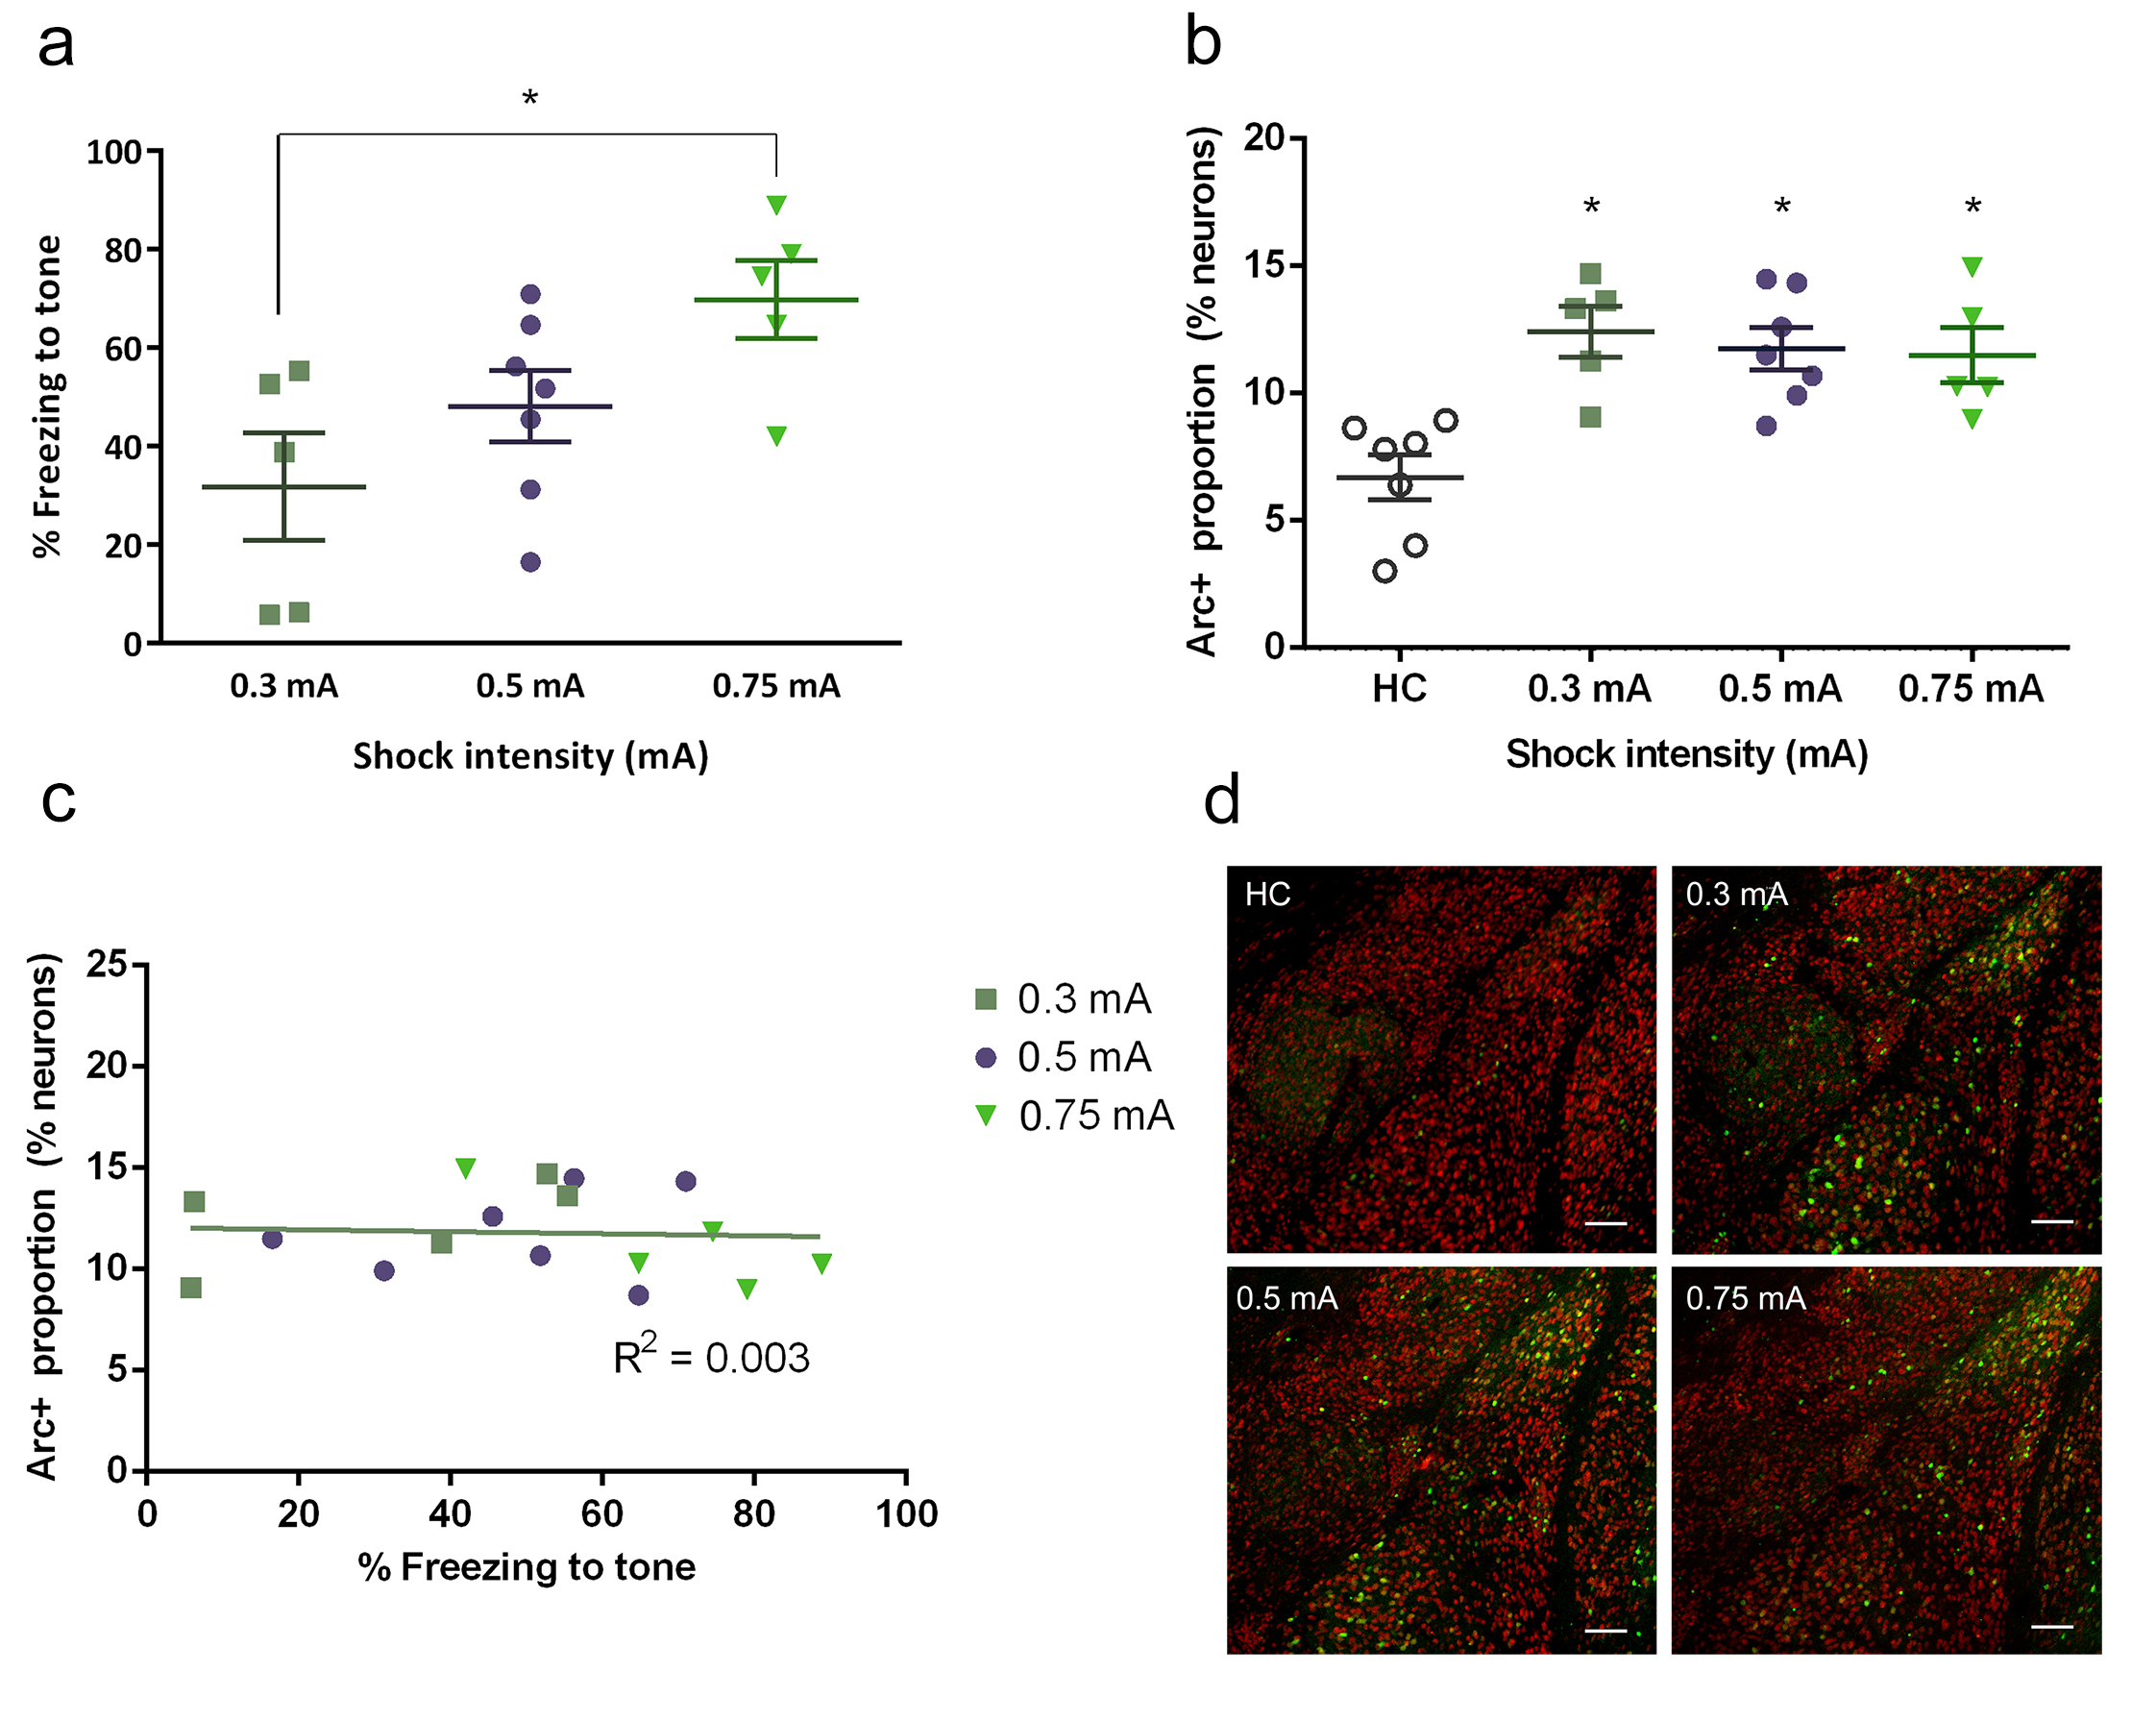
\includegraphics{source/figures/figure_2.jpg}
\caption{\textbf{Consistent proportion of Arc+ neurons in the LA
following auditory fear retrieval despite varying degrees of freezing.}
(a) Increasing shock intensity during training produced higher levels of
freezing during the test, consistent with greater fear memory. (b) The
proportion of Arc+ neurons was increased following testing, but no
difference in Arc+ proportion was observed between groups trained with
varying intensities of shock. (c) No relationship was seen between time
spent freezing to tone and Arc+ proportion. (d) Examples of Arc (green)
and NeuN (red) staining in the LA of HC mice and those treated with
varying shock intensity. Scale bars, 50 μm. (HC, n = 7; 0.3 mA footshock
intensity, n = 5; n = 7, 0.5 mA; n = 5, 0.75 mA). * P \textless{} 0.05
with Tukey's post hoc test for multiple comparisons. Data is expressed
as mean ± sem. \label{ref_a_figure}}
\end{figure}

\section{\texorpdfstring{\emph{Arc} mRNA increases in a stable
proportion of LA neurons during fear
conditioning}{Arc mRNA increases in a stable proportion of LA neurons during fear conditioning}}\label{arc-mrna-increases-in-a-stable-proportion-of-la-neurons-during-fear-conditioning}

In order to gain a more temporally precise measure of the engram, we
performed cellular compartmental analysis of temporal activity by
fluorescence in situ hybridization (catFISH) to identify LA neurons
expressing \emph{Arc} mRNA during either encoding or retrieval or of an
auditory fear memory. Expression of \emph{Arc} mRNA in the nucleus peaks
within 5 minutes of neural activity (John F. Guzowski et al., 2005),.
Thus, by sacrificing animals 5 minutes after auditory fear training or
testing, it was possible to to identify active neuronal ensembles with a
high degree of temporal accuracy. Although different training conditions
produced varying degrees of freezing to the tone (Figure 4.3a; F(2, 7) =
5.30, P \textless{} 0.05), there was no difference in the proportion of
\emph{Arc}\textsuperscript{+} cells between any groups exposed to fear
conditioning (Figure 4.3b; F(4, 10) = 0.99, P \textgreater{} 0.05).
Furthermore, no difference was observed in the number of
\emph{Arc}\textsuperscript{+} neurons between brains examined after
training or testing. All groups that received training differed from the
immediate shock control, which exhibited very low \emph{Arc} signal (all
groups vs immediate shock, P \textless{} 0.001). No relationship was
observed between \emph{Arc}\textsuperscript{+} proportion and percentage
time spent freezing (Figure 4.3c, R2 = 0.096), suggesting that the
proportion of LA neurons that are strongly activated during memory
encoding and retrieval 24 hr later is unrelated to the strength of
learned associations.

\begin{figure}[htbp]
\centering
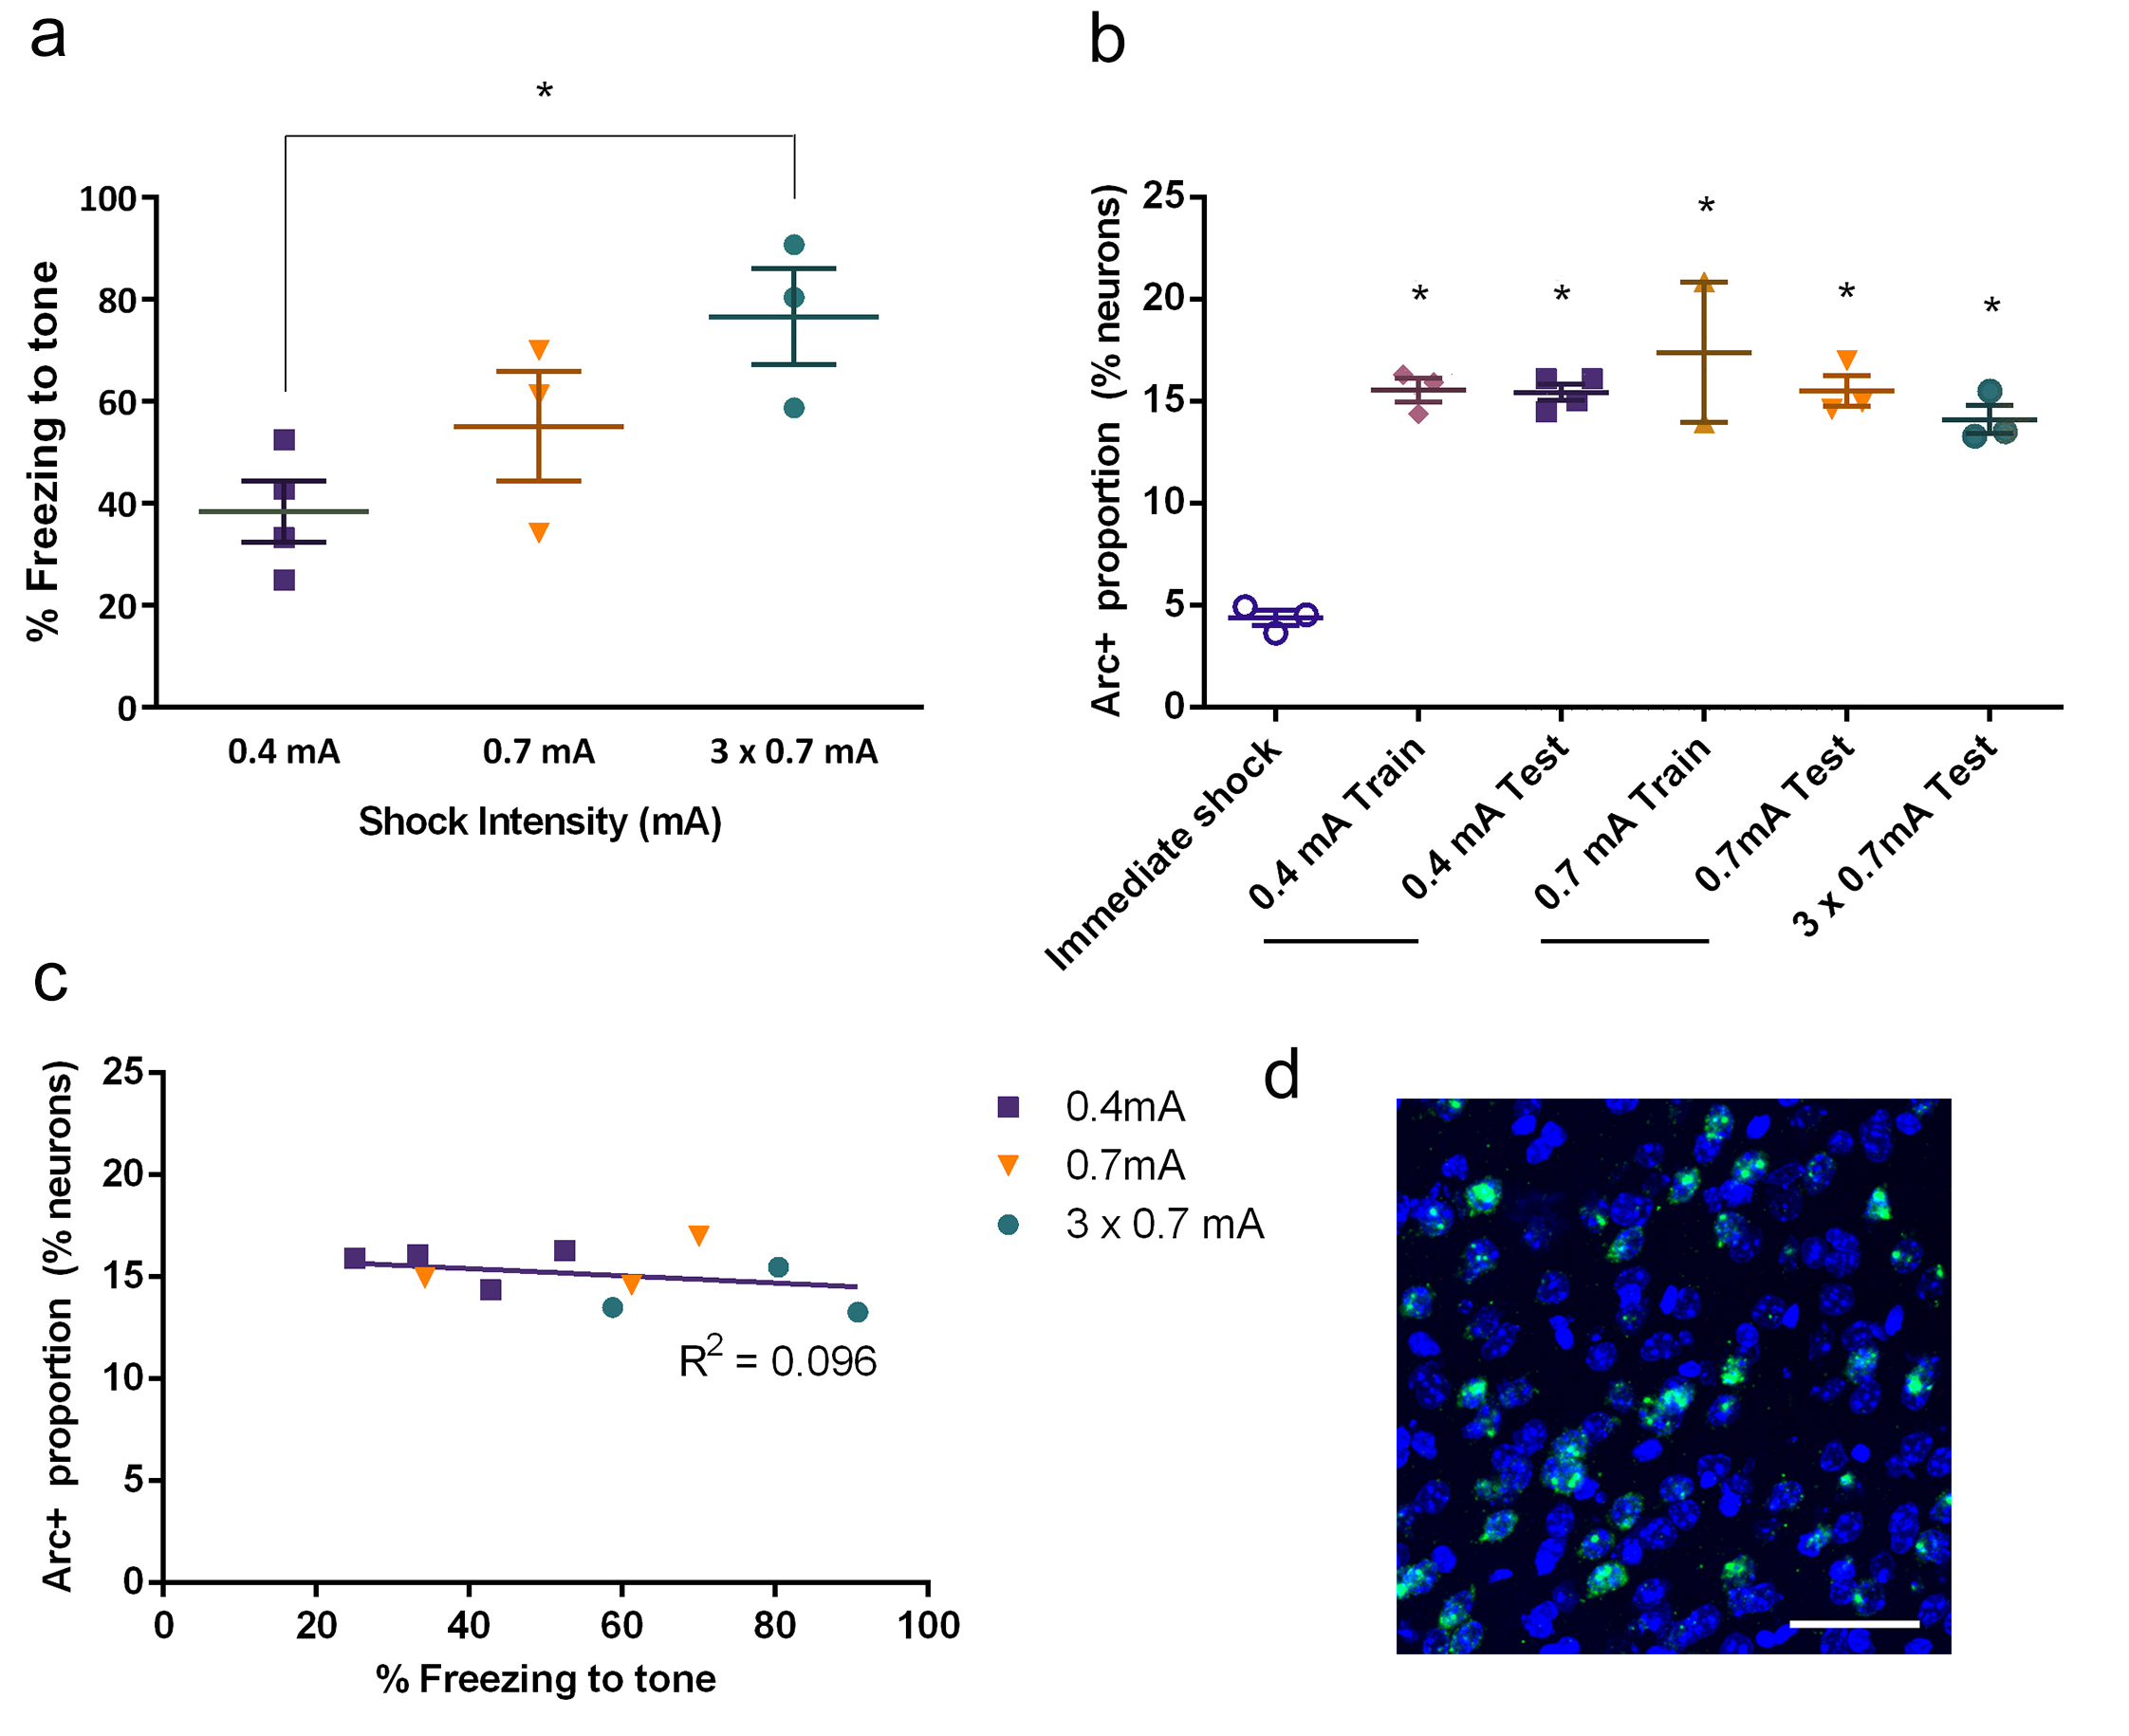
\includegraphics{source/figures/figure_3.jpg}
\caption{\textbf{Consistent proportion of cells expressing \emph{Arc}
mRNA in the LA following auditory fear retrieval despite varying degrees
of freezing} (a) Increased shock intensity produced greater time spent
freezing to tone during testing. (b) No difference in \emph{Arc+}
proportion was observed between groups trained with varying intensities
of shock (c) No relationship was seen between time spent freezing to
tone and \emph{Arc+} proportion within mice. (d) Example of catFISH
staining for \emph{Arc} (green) and Hoescht (blue) in the LA. Scale bar,
50 μm. (n = 3, immediate shock; n = 3, 0.4 mA Train; n = 4, 0.4 mA Test;
n = 2, 0.7 mA Train; n = 3, 0.7 mA Test; n = 3, 3 x 0.7 mA Test). * P
\textless{} 0.05 with Tukey's post hoc test for multiple comparisons.
Data is expressed as mean ± sem. \label{ref_a_figure}}
\end{figure}

\section{\texorpdfstring{Inhibition of PV\textsuperscript{+}
interneurons during conditioning increases the size of the lateral
amygdala
engram}{Inhibition of PV+ interneurons during conditioning increases the size of the lateral amygdala engram}}\label{inhibition-of-pv-interneurons-during-conditioning-increases-the-size-of-the-lateral-amygdala-engram}

In both the LA and the basal amygdala (BA), local inhibition is
predominantly mediated by GABAergic parvalbumin (PV) interneurons
(Ehrlich et al., 2009, Spampanato et al. (2011)), which form a broad,
inter-connected inhibitory network that responds to sensory input
(Szinyei et al., 2000) and tightly controls the activity of LA principal
neurons through plastic, perisomatic synapses (Freund \& Katona (2007),
Trouche, Sasaki, Tu, \& Reijmers (2013)). Because of this,
PV\textsuperscript{+} interneurons represent a promising candidate for
mediating inhibitory interactions between principal neurons. To
determine whether PV\textsuperscript{+} interneurons play a role in
constraining the size of the LA engram, we used inhibitory DREADDS
(designer receptors exclusively activated by designer drugs) to silence
their activity during training. DREADDS are modified G-protein coupled
receptors activated by the synthetic ligand clozapine-N-oxide (CNO) that
allow neuronal activity to be modulated over prolonged periods (Nichols
\& Roth, 2009). The inhibitory DREADD hM4D was selectively targeted to
PV-containing cells in the amygdala through the use of a Cre-dependent
adeno-associated viral vector (AAV-DIO-hM4Di-mCherry) infused into the
amygdala in transgenic mice (PV-Cre knockin). This technique ensured
that an inhibitory receptor was expressed only in PV\textsuperscript{+}
cells of the amygdala (Tanahira et al., 2009). CNO or a vehicle (VEH)
control was systemically administered 1 hr before auditory fear
conditioning with a 0.5 mA footshock to inhibit PV\textsuperscript{+}
cells during memory encoding. The next day, animals were sacrificed 90
min after testing in a novel context and immunohistochemistry for Arc
protein was performed.

Inhibiting PV\textsuperscript{+} interneurons during auditory fear
conditioning increased the number of neurons allocated to the LA
component of the engram. No difference in freezing behavior between
animals treated with CNO or VEH (Figure 4.4a; unpaired t test, P
\textgreater{} 0.5) was observed, but mice treated with CNO displayed an
increased proportion of Arc\textsuperscript{+} cells in the LA (Figure
4.4b; P \textless{} 0.01; Mann-Whitney U test, P \textless{} 0.05). No
relationship was observed between percentage of time spent freezing and
Arc\textsuperscript{+} proportion (Figure 4.4c; CNO, R2 = 0.015; VEH R2
\textless{} 0.001). Together, these findings suggest that reduced
PV\textsuperscript{+} interneuron activity during auditory fear
conditioning increases the number of cells allocated to the engram
without influencing memory strength.

\begin{figure}[htbp]
\centering
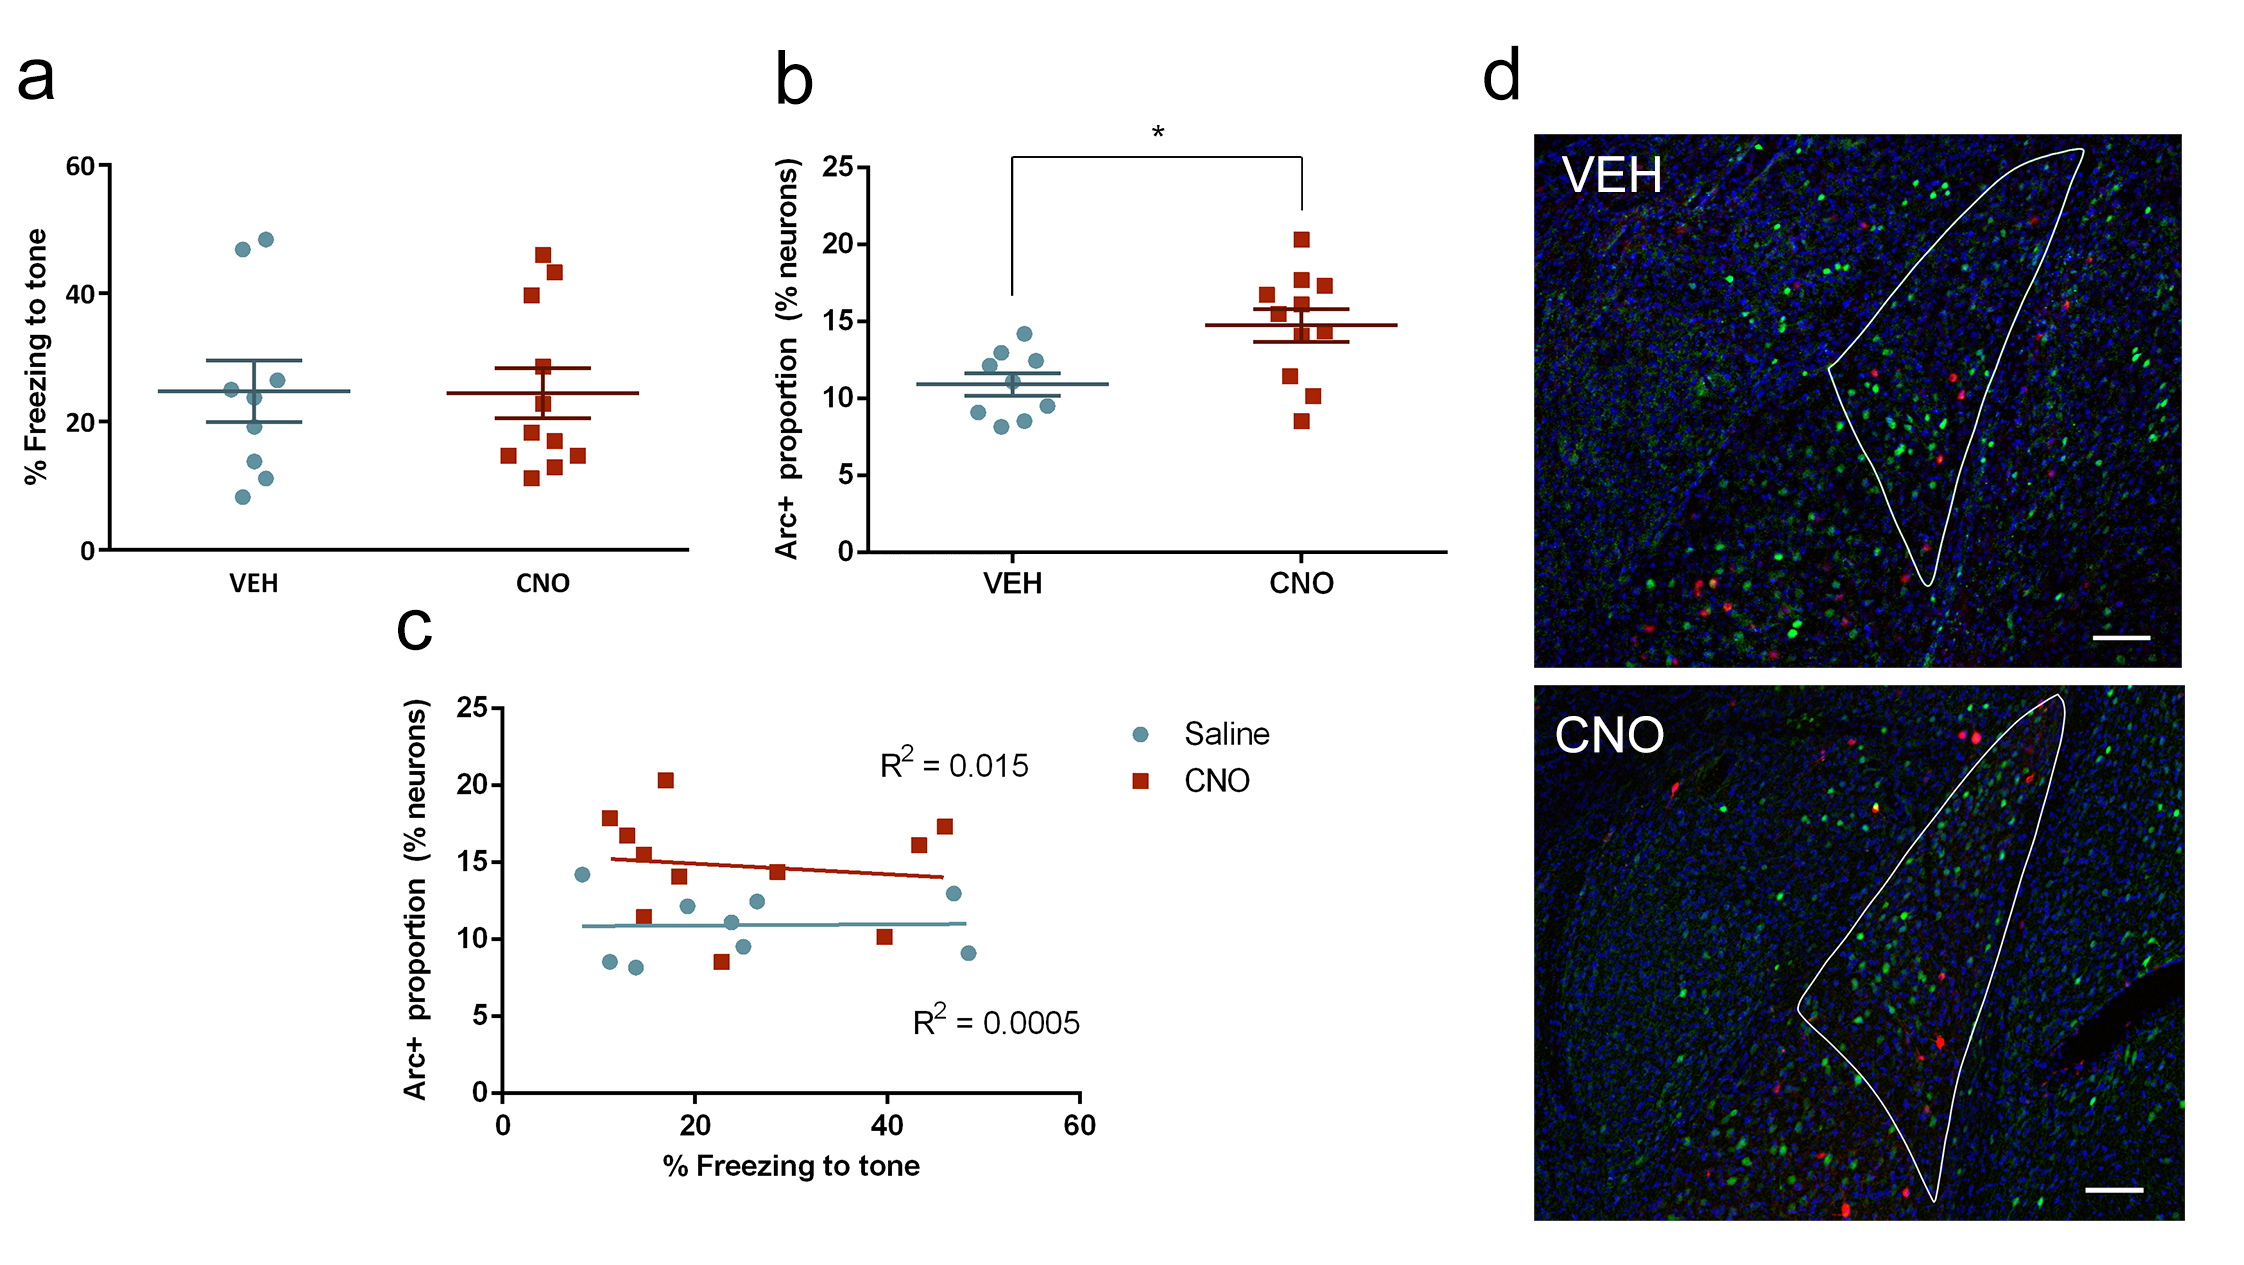
\includegraphics{source/figures/figure_4.jpg}
\caption{\textbf{PV+ inhibition during auditory fear conditioning
increases the proportion of Arc+ neurons during subsequent retrieval.}
(a) Both groups treated with CNO and VEH showed similar freezing to
tone. (b) The proportion of Arc+ neurons in the LA was greater in mice
treated with CNO. (c) No relationship was seen between freezing
behaviour and Arc+ proportion in mice treated with VEH or CNO. (d)
Representative images of sections with virally infected PV+ interneurons
expressing mCherry (red), Arc (green), and DAPI (blue). The LA is
outlined. (n = 9, VEH; n = 11, CNO). * P \textless{} 0.05. Data is
expressed as mean ± sem. \label{ref_a_figure}}
\end{figure}

The LA can be subdivided into distinct subnuclei on the basis of
extra-amygdalar connectivity (Romanski et al., 1993; P. Sah et al.,
2003). To explore whether the allocation of neurons to the engram in our
experiments varied depending upon their location within the LA,
stereological estimates of Arc\textsuperscript{+} proportion in PV-Cre
mice treated with CNO or VEH were divided among the dorsal (LAd),
ventral-medial (LAvm), and ventral-lateral (LAvl) subnuclei (Figure
4.5a). This analysis revealed that Arc\textsuperscript{+} proportion
varied between these regions in animals treated with CNO (Figure 4.5B; P
\textless{} 0.05), but not in the VEH group (P \textgreater{} 0.05).
Furthermore, the LAd, which had the greatest proportion of
Arc\textsuperscript{+} cells in CNO-treated animals, was also the only
subnucleus in which we observed a difference following
PV\textsuperscript{+} inhibition (unpaired t test, P \textless{} 0.01).
These findings suggest that the increase in the size of the engram we
observed could have been driven exclusively by changes in the
recruitment of LAd neurons.

\begin{figure}[htbp]
\centering
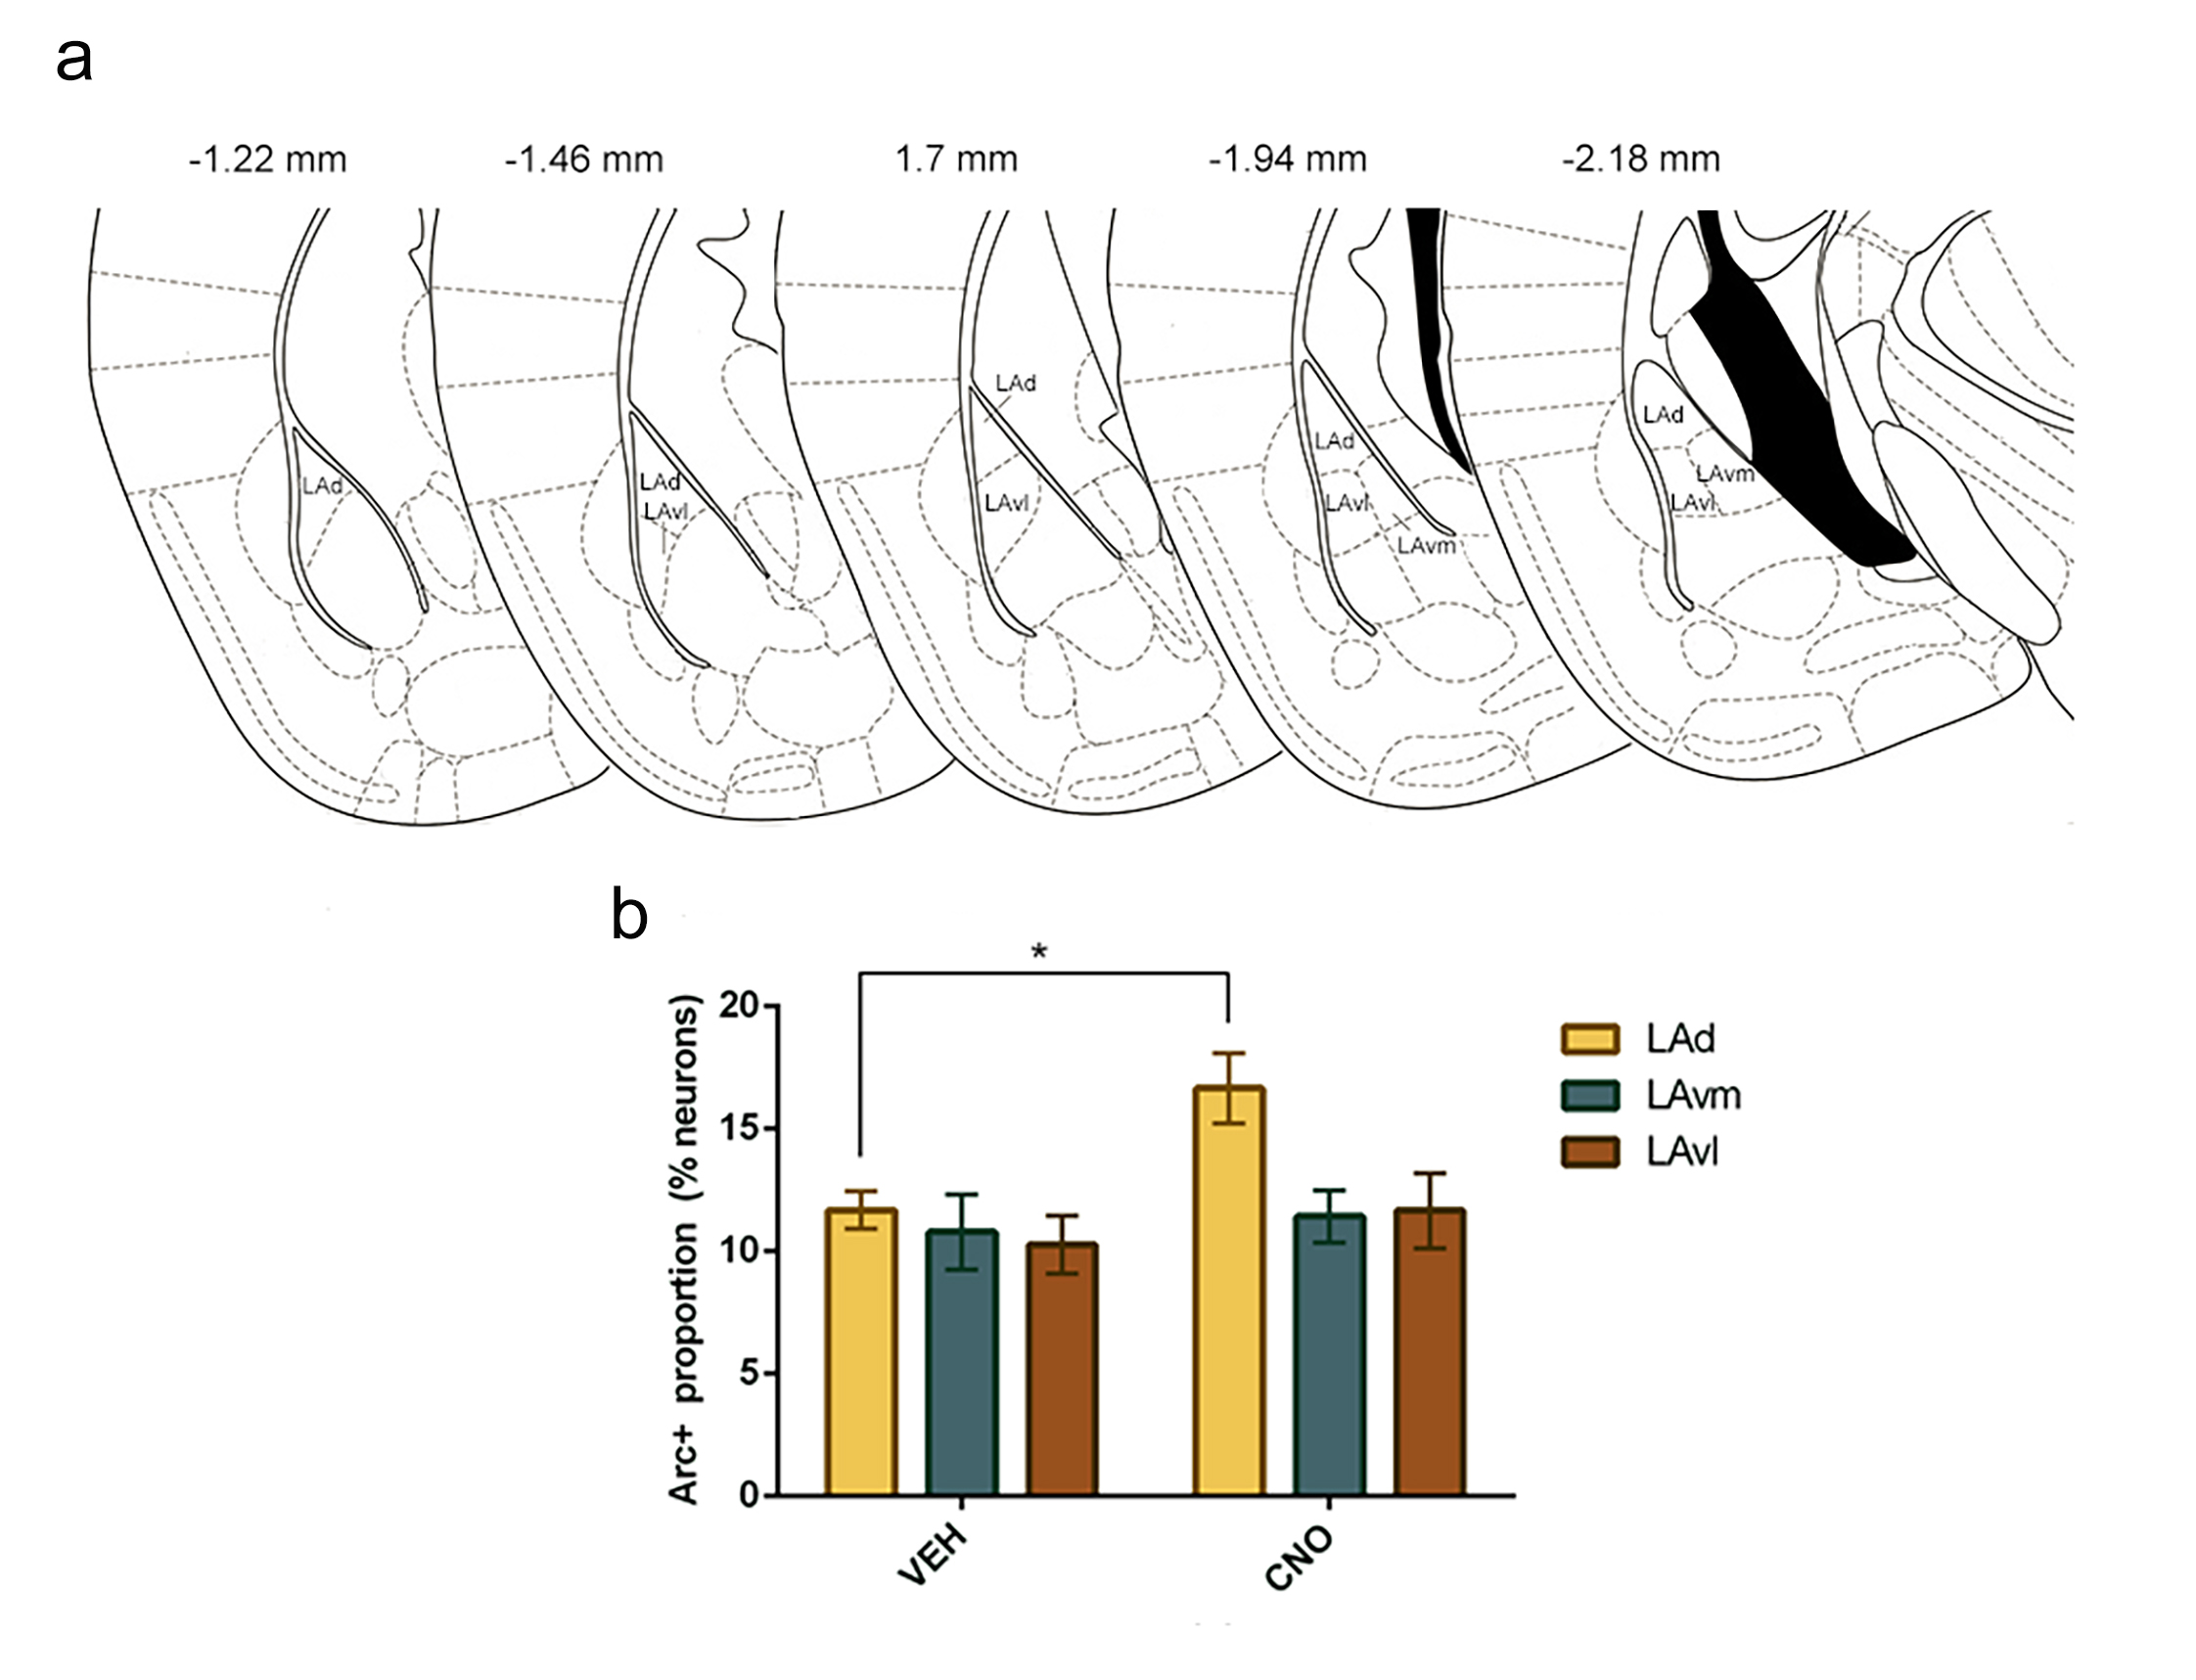
\includegraphics{source/figures/figure_5.jpg}
\caption{\textbf{Inhibition of PV+ cells increases the proportion of
Arc+ cells in the LAd} (a) Anatomy of the amygdala from anterior (-1.22
mm from bregma) to posterior (-2.18 mm) illustrating the distinction
between the LAd, LAvm, and LAvl. Adapted from Paxinos and Franklin. (b)
The LAd contained a higher proportion of Arc+ cells in animals treated
with CNO and was the only subnucleus in which a difference in Arc+
proportion was observed when compared to VEH controls (n = 9, VEH; n =
11, CNO). * P \textless{} 0.05 with unpaired Student's t test. Data is
expressed as mean ± sem. \label{ref_a_figure}}
\end{figure}

\chapter{Research containing a
figure}\label{research-containing-a-figure}

\section{Introduction}\label{introduction-3}

This is the introduction. Sed vulputate tortor at nisl blandit interdum.
Cras sagittis massa ex, quis eleifend purus condimentum congue. Maecenas
tristique, justo vitae efficitur mollis, mi nulla varius elit, in
consequat ligula nulla ut augue. Phasellus diam sapien, placerat sit
amet tempor non, lobortis tempus ante.

\section{Method}\label{method-1}

Donec imperdiet, lectus vestibulum sagittis tempus, turpis dolor euismod
justo, vel tempus neque libero sit amet tortor. Nam cursus commodo
tincidunt.

\subsection{Subsection 1}\label{subsection-1}

This is the first part of the methodology. Duis tempor sapien sed tellus
ultrices blandit. Sed porta mauris tortor, eu vulputate arcu dapibus ac.
Curabitur sodales at felis efficitur sollicitudin. Quisque at neque
sollicitudin, mollis arcu vitae, faucibus tellus.

\subsection{Subsection 2}\label{subsection-2-1}

This is the second part of the methodology. Sed ut ipsum ultrices,
interdum ipsum vel, lobortis diam. Curabitur sit amet massa quis tortor
molestie dapibus a at libero. Mauris mollis magna quis ante vulputate
consequat. Integer leo turpis, suscipit ac venenatis pellentesque,
efficitur non sem. Pellentesque eget vulputate turpis. Etiam id nibh at
elit fermentum interdum.

\section{Results}\label{results-2}

These are the results. In vitae odio at libero elementum fermentum vel
iaculis enim. Nullam finibus sapien in congue condimentum. Curabitur et
ligula et ipsum mollis fringilla.

\section{Discussion}\label{discussion-1}

Figure \ref{ref_a_figure} shows how to add a figure. Donec ut lacinia
nibh. Nam tincidunt augue et tristique cursus. Vestibulum sagittis odio
nisl, a malesuada turpis blandit quis. Cras ultrices metus tempor
laoreet sodales. Nam molestie ipsum ac imperdiet laoreet. Pellentesque
habitant morbi tristique senectus et netus et malesuada fames ac turpis
egestas.

\begin{figure}[htbp]
\centering
\includegraphics{source/figures/example_figure.pdf}
\caption{RV Calypso is a former British Royal Navy minesweeper converted
into a research vessel for the oceanographic researcher Jacques-Yves
Cousteau. It was equipped with a mobile laboratory for underwater field
research. \label{ref_a_figure}}
\end{figure}

\section{Conclusion}\label{conclusion-2}

This is the conclusion to the chapter. Quisque nec purus a quam
consectetur volutpat. Cum sociis natoque penatibus et magnis dis
parturient montes, nascetur ridiculus mus. In lorem justo, convallis
quis lacinia eget, laoreet eu metus. Fusce blandit tellus tellus.
Curabitur nec cursus odio. Quisque tristique eros nulla, vitae finibus
lorem aliquam quis. Interdum et malesuada fames ac ante ipsum primis in
faucibus.

\chapter{Discussion}\label{discussion-2}

\section{Summary of Findings}\label{summary-of-findings}

Memories are thought to be represented in the brain by discrete
biophysical changes (Eichenbaum, 2016, Josselyn, Köhler, \& Frankland
(2015), Tonegawa, Liu, Ramirez, \& Redondo (2015)). These changes,
collectively referred to as an engram, are widely distributed throughout
the brain and include a range of alterations, from epigenetics to
synaptic connectivity and neural excitability. Although little is known
about how information is encoded within engrams (Eichenbaum, 2016),
recent studies have shown that neurons active during learning are
recruited into sparse ensembles whose reactivation at later time points
is necessary and sufficient for memory recall (Han et al., 2009, J. Kim,
Kwon, Kim, Josselyn, \& Han (2013), Liu et al. (2012)). In the amygdala,
these ensembles are primarily composed of those cells that were most
strongly activated by the stimuli present during learning, with the
results of some studies indicating that the size of these neuronal
ensembles is constrained by mechanisms that allocate only a proportion
of the most excitable cells to the engram ((Han et al., 2007, Yiu et al.
(2014)). Theoretical studies investigating this process of competitive
memory allocation have suggested that this constraint facilitates the
implementation of efficient, specific memory representations (Feng et
al., 2016). However, empirical evidence for the mechanisms that mediate
this constraint has not yet been collected.

In this work, I have examined the process of engram formation in the LA
and attempted to prove that inhibitory interneurons constrain the number
of neurons allocated to the engram to a sparse trace. First, I
demonstrated that the immediate early gene Arc can be used to visualize
neurons allocated to the engram of an auditory fear memory in the LA.
Second, I demonstrated that the LA component of an engram remains stable
despite variations in the strength of the memory. Lastly, I tested
whether inhibitory PV\textsuperscript{+} interneurons in the amygdala
are involved in memory allocation by inhibiting their activity during
auditory fear conditioning. I observed that the inhibition of
PV\textsuperscript{+} interneurons increased the size of the LA engram,
confirming predictions made in modeling studies regarding the role of
inhibitory interneurons in mediating a process of competition between
neurons during memory encoding that constrains the engram to a sparse
population.

\section{The use of IEGs to identify the
engram}\label{the-use-of-iegs-to-identify-the-engram}

There is a wide variety of techniques used in neuroscience to measure
the activity of the brain. One such technique involves the use of
immediate early genes (IEGs). IEG analysis allows researchers that study
the brain in fine morphological detail with fixed tissue histology and
microscopy to obtain a rough estimate of neural activity by exploiting
the fact that many genes are reliably transcribed and translated into
protein following intense neural activity. When examining fixed brain
tissue specimens, immunohistochemical staining for these genes permits
the cells that were most active in the period of time directly before
fixation to be identified. Genes used for IEG analysis share a number of
common properties. Crucially, they are all expressed constitutively at
very low levels, but increase their expression rapidly and dramatically
following the types of high frequency activity associated with synaptic
plasticity and neural encoding (J. F. Guzowski, McNaughton, Barnes, \&
Worley, 1999). The physiological function of these genes is diverse, but
many are involved in synaptic plasticity and other processes that allow
neurons to modify their function in response to external input (John F.
Guzowski et al., 2005). Genes used for IEGs also tend to be highly
conserved across species, making them appropriate targets for study in a
wide variety of animal models.

Activity-regulated cytoskeletal-associated protein (Arc) is an IEG that
has the specific advantage of being selectively expressed only in
excitatory principal neurons (Vazdarjanova et al., 2006). Arc interacts
with the synaptic machinery of receptor endocytosis to metaplastically
regulate synapses that have recently undergone long-term potentiation
(Bramham et al., 2010), and although its function has not been fully
described, it has been used in a large body of work to identify neurons
participating in engrams based on their activity during memory encoding
or retrieval (Gouty-Colomer et al., 2015, Liu et al. (2012), Reijmers et
al. (2007), Tayler et al. (2013)).

\section{Arc expression increases during training and
testing}\label{arc-expression-increases-during-training-and-testing}

In order to validate the use of Arc to measure engrams in this study,
immunohistochemistry for Arc was performed after either auditory fear
training or testing the density of Arc\textsuperscript{+} cells compared
to treatment groups in which no training was given (homecage) or in
non-learning control groups (tone only, context only, immediate shock).
In all but the intercalated cell masses, the density of
Arc\textsuperscript{+} cells was greater in animals sacrificed after
either training or testing than any control groups, suggesting that the
increase in Arc across the LA seen during training and testing was
specifically due to the activation of neuronal ensembles involved in the
encoding and retrieval of an associative memory. It was also determined
that the density of Arc\textsuperscript{+} cells was equivalent between
testing and training conditions within all brain regions, consistent
with the hypothesis that similar patterns of activity are induced in the
brain during both encoding and retrieval (Reijmers et al., 2007, Tayler
et al. (2013)).

The increase in Arc seen throughout the amygdala is highly consistent
with the current understanding of the storage and retrieval of fearful
memories. Although the LA, which acts as the primary sensory interface
of the amygdala contains the essential components of the engram for
encoding sensory associations, activity in the BA and CeA is thought to
underlie the inclusion of contextual details and fear expression,
respectively (Tovote, Fadok, \& Lüthi, 2015). The lack of Arc response
seen in the intercalated cell masses is likely due to the fact that they
are primarily composed of GABAergic interneurons (Ehrlich et al., 2009),
which do not express Arc (Vazdarjanova et al., 2006).

\section{Stereological counting to measure the
engram}\label{stereological-counting-to-measure-the-engram}

In order to accurately measure the proportion of neurons allocated to an
engram, unbiased, systematic stereological procedures were used. By
systematically drawing samples from a large population, the practice of
stereology allows geometrical quantities to be estimated without
sacrificing accuracy or efficiency. When attempting to measure the
number of cells in a region of the brain, exhaustive counting of dense
cellular populations becomes formidably time-consuming. In addition,
sectioning tissue often leads to cell fragments, which can produce
estimates of cell number that differ from the true number of cells
present. Stereological techniques overcome these issues by drawing
samples for counting from a large total volume in a statistically
unbiased way, so the density of cells within a smaller counted area can
be extrapolated to represent the larger volume.

To obtain an accurate ratio of Arc\textsuperscript{+} to total neurons
in the LA, serial sections were analyzed using optical fractionation.
Optical fractionation begins with the collection of serial sections
throughout the region of interest, followed by the systematic random
distribution of three-dimensional counting frames within those sections.
The distance between sections and the size and density of counting
frames is determined before the experiment begins in order to achieve an
appropriate level of statistical accuracy (West, Slomianka, \&
Gundersen, 1991).

\section{Memory retrieval activates a constant proportion of cells in
the amygdala despite varying memory
strength}\label{memory-retrieval-activates-a-constant-proportion-of-cells-in-the-amygdala-despite-varying-memory-strength-1}

The hypothesis that competitive inhibitory interactions enforce sparsity
within the LA engram suggests that all memories will be distributed
among neural ensembles of the same size, regardless of the content or
intensity of those memories. One way to test whether this is the case is
to manipulate memory strength (ie. the distinctiveness and/or intensity
of learned associations) and investigate whether this alters the number
of neurons allocated to the engram. Because the strength of Pavlovian
conditioning memories is a function of the valence of the US and the
salience of the CS (Itzhak, Perez-Lanza, \& Liddie, 2014), maniplations
of the intensity of US footshock delivered during auditory fear
conditioning was explored as a method to increase fear memory strength.
Indeed, increasing footshock was associated with greater time spent
freezing to the tone 24 hrs after training.

Stereological counting of the proportion of neurons active during
retrieval did not reveal a relationship between memory strength and the
size of the engram. All animals that showed elevated freezing during
tone presentation displayed a higher degree of Arc labeling in the LA
compared to animals that remained in their homecage, indicating that
successful retrieval of a fear association was associated with
reactivation of a small subset of LA neurons. However, there was no
difference in the size of this population between groups trained with
low (0.3 mA), medium (0.5 mA), or high (0.75 mA) footshock. Furthermore,
no relationship was seen between an animal's degree of freezing to the
tone and the proportion of Arc\textsuperscript{+} cells in the LA. These
results suggest that all auditory fear engrams are stored in similarly
sized populations of neurons in the LA (\textasciitilde{}12\% in these
experiments).

These findings do not preclude the existence of differences between the
LA engrams of strong or weak memories. Rather, they only suggest that it
is the number of neurons involved that remains constant. There are many
components of the engram that the approach taken in this study was
unable to detect and it is possible that characteristics of
similarly-sized memory ensembles may vary along these other dimensions.
Indeed, it has been shown that engram neurons are more intensely
activate during the retrieval of strong memories (Gouty-Colomer et al.,
2015). Furthermore, it is possible that the size of engrams in the LA
may change over time and that the number of neurons activated during
retrieval may be reduced due to extinction or consolidation. One
previous study that reported a positive relationship between the
strength of auditory fear memory and the number of reactivated neurons
in the LA did so only after extinction training (Reijmers et al., 2007).
Thus, it is possible that the number of reactivated neurons in the
engram may bear a significant relation to memory strength in conditions
in which the memory trace has been degraded or suppressed. Decreased
memory strength in such conditions could reflect a failure in
autoassociative retrieval within the LA network, which would manifest as
a lower proportion of activated neurons.

\section{mRNA as a time sensitive marker of neuronal
activity}\label{mrna-as-a-time-sensitive-marker-of-neuronal-activity}

The primary limitation of protein-based IEG techniques for identifying
the engram is an extremely poor temporal resolution. Protein expression
occurs over a period of minutes and hours, whereas the
sensory-behavioural events that IEG approaches attempt to investigate
occur often over a time period of seconds. Thus protein-based labeling
often capture cells not only neurons active during a behavioural epoch
of interest, but also those active during a broad period of time before
and after. This drawback has been suggested to underlie some of the
surprisingly low estimates of overlap between neural populations active
during encoding and retrieval in previous studies (Josselyn et al.,
2015).

One technique that is can be used to overcome the limited temporal
resolution of protein-based IEG analysis is cellular compartmental
analysis of temporal activity by fluorescence in situ hybridization
(catFISH), which labels IEG mRNAs. This technique benefits from the fact
that mRNA transcription in the nucleus begins much earlier than changes
in protein expression after neural activity and has been shown to be
able to identify increases in Arc mRNA associated with high frequency
activity in as little as 2 mins (John F. Guzowski et al., 2005 ). This
stands in stark contrast to Arc protein expression, which does not peak
until 60-90 minutes after activity. The catFISH technique also allows
multiple time points of activity to be detected due to the fact that
mRNA transcripts produced in the nucleus transit to the dendrites to be
expressed: dendritic Arc indicates activity between 20-60 min ago while
nuclear Arc indicates activity with \textless{} 16 min.

\section{Arc mRNA reveals sparse activation of LA neurons during fear
memory
retrieval}\label{arc-mrna-reveals-sparse-activation-of-la-neurons-during-fear-memory-retrieval}

In order to demonstrate that the stable proportion of engram cells
observed with multiple shock conditions was not due to an over-inclusive
labeling technique, catFISH and stereological counting was performed to
determine the proportion of neurons activated within a narrow time
window around encoding or retrieval of an auditory fear memory. This
investigation produced a similar result as the previous investigation
involving protein-based IEGs. Increased shock intensity was associated
with more strongly expressed memories, but there was no difference in
the size of the LA component of the engram between any group during
training or testing. This suggest that, even when correcting for the
temporal inaccuracy of protein-based IEGs, the proportion of neurons
allocated to the engram in memories of different strengths remains
constant.

Interestingly, despite the narrow temporal window afforded by catFISH, a
similar, slightly greater, proportion of engram neurons (15\%) was
recorded in comparison to experiments involving protein-based IEG, even
when only cells with intranuclear fluorescence were counted. It is
unclear whether the smaller time window of capture was offset by a lower
threshold of detection with catFISH, or whether the previous protein
based IEG analysis was simply accurate enough. However, the relative
similarity in estimates of the engram population between this mRNA-based
approach, protein-based results, and the multitude of other studies on
engram size (An et al., 2012, Ghosh \& Chattarji (2015), Gouty-Colomer
et al. (2015), Herry et al. (2008), Quirk et al. (1995)) provide further
support for the hypothesis that memory traces are actively constrained
to a sparse population and validation of this experimental approach
involving Arc.

\section{DREADDS to manipulate cellular
excitability}\label{dreadds-to-manipulate-cellular-excitability}

In order to selectively modulate the activity of PV\textsuperscript{+}
interneurons during the acquisition of fear memories, designer receptors
exclusively activated by designer drugs (DREADDs) were targeted to
PV-expressing neurons with a Cre-dependent viral vector. DREADDs are
modified G-protein coupled receptors that are activated by a specific
synthetic ligand, clozapine-N-oxide (CNO), that otherwise has no
activity in the body (Armbruster, Li, Pausch, Herlitze, \& Roth, 2007).
Several varieties of DREADDs have been created that have different
functions on neural activity. The DREADD subtype used in this
investigation, hM4Di, is an inhibitory receptor that decreases cellular
activity by lowering the activity of cAMP, reducing potassium channel
conductance, and inhibiting presynaptic neurotransmitter release.

DREADDs allow neural activity to be modulated over a time-scale that is
both appropriate and highly convenient for behavioural neurobiological
experiments. When CNO is injected intraperitoneally, DREADD activation
begins within minutes, peaks after 50 minutes, and dissipates several
hours later (Alexander et al., 2009). This provides a sufficiently large
time window for behavioural experiments to be performed while also
ensuring that experiments performed the following day are free of the
effects of lingering DREADD activity. The consequences of the prolonged
neural modulation that DREADDs provide during the few hours that CNO is
present are not entirely understood, however. Dramatic differences in
outcomes between studies that used prolonged, pharmacological
manipulations and precise optogenetic approaches have been identified
(Goshen et al., 2011), and it may be possible that the brain is able to
compensate for the effect of DREADDs in some way.

\section{\texorpdfstring{Inhibition of PV\textsuperscript{+}
interneurons increases the size of the LA
engram}{Inhibition of PV+ interneurons increases the size of the LA engram}}\label{inhibition-of-pv-interneurons-increases-the-size-of-the-la-engram}

Computational modeling of memory formation in the LA has suggested that
competitive interactions mediated by inhibitory interneurons are
necessary for maintaining the size of memory traces despite variations
in excitability (Feng et al., 2016). In order to empirically test this
hypothesis, DREADDS were selectively targeted to PV-containing
interneurons in the amygdala with the use of PV-Cre transgenic mice and
a Cre-dependent viral vector. This allowed a proportion of
PV\textsuperscript{+} interneurons to be inhibited during auditory fear
conditioning to assess their role in constraining the size of the engram
in the LA. Of the many interneuron subtypes present, we focused on
PV\textsuperscript{+} interneurons because of their implication in the
regulation of principal neuron excitability (Spampanato et al., 2011)
and the modulation of fear memories (Trouche et al., 2013).

Remarkably, inhibiting PV\textsuperscript{+} cells during training
increased the number of neurons allocated to the engram (Figure 4),
suggesting that they may play some role in the mechanisms that govern
the formation of neuronal ensembles during memory encoding. This
increase was modest (11 --\textgreater{} 15\%), but represented the fact
that engrams were 35\% larger when formed under conditions of reduced
PV\textsuperscript{+} activity. Although this investigation is unable to
describe exactly how this expansion in the memory trace occurred, these
results corroborate modeling studies regarding the importance of
inhibitory interneurons in making memory allocation a competitive
process (Dongbeom Kim, Paré, \& Nair, 2013b, Feng et al. (2016)), the
most recent of which specifically proposed that decreases in the
plasticity of inhibitory connections would lead to an increase in the
number of cells that undergo plasticity during fear conditioning.

These results do not preclude the fact that other interneuron subtypes
may also be involved in constraining the size of the engram (Stefanelli,
Bertollini, Lüscher, Muller, \& Mendez, 2016). Indeed, it may be
possible that this increase in the size of the engram observed during
PV\textsuperscript{+} interneuron inhibition was due to a disruption of
the PV\textsuperscript{+} and SOM\textsuperscript{+} microcircuits that
shape the flow of sensory input (Wolff et al., 2014). It may also have
been the case that reducing inhibitory PV\textsuperscript{+} cell firing
made the LA more excitable and increased the number of neurons that were
excited above plasticity thresholds. However, in light of existing work
demonstrating the competitive nature and remarkable stability of the LA
engram, as well as computational models predicting the existence of
competitive inhibitory interactions, it is perhaps best to assume that
this finding has at least significantly advanced the hypothesis that
interneurons play some role in the formation of memory engrams.

\section{\texorpdfstring{Subnuclear location of PV\textsuperscript{+}
inhibition-related engram
increase}{Subnuclear location of PV+ inhibition-related engram increase}}\label{subnuclear-location-of-pv-inhibition-related-engram-increase}

In order to understand the nature of these findings in light of the
anatomical distinctions that have been proposed between the LA's dorsal
(LAd), ventral-medial (LAvm), and ventral-lateral (LAvl) subnuclei
(Romanski et al., 1993, sah\_amygdaloid\_2003), the stereological
results of this experiment involving PV\textsuperscript{+} cell
inhibition were divided up between these regions to obtain independent
estimates of Arc\textsuperscript{+} proportion. These three subdivisions
of the LA have been shown to receive different forms of innervation from
the rest of the brain, with the LAd receiving the majority of fast,
thalamic, auditory projections and the ventral regions receiving slower,
cortical inputs (Romanski et al., 1993). Thus, it is possible that
salient sensory information encoded during auditory fear conditioning
may be differentially allocated across these regions.

Interestingly, analyzing the proportion of Arc\textsuperscript{+}
neurons across these subnuclei revealed that a significantly higher
proportion of neurons were allocated to the memory trace in the LAd in
animals in which PV\textsuperscript{+} interneurons were inhibited
during training (Figure 5). Furthermore, this increase in
Arc\textsuperscript{+} proportion in the LAd accounted for the majority
of the increased size of the engram, suggesting that
PV\textsuperscript{+} interneurons may play a more significant role in
regulating the excitability of LAd neurons. Indeed, it has been noted
that the ratio of excitatory to inhibitory inputs is lower in more
dorsally located neurons in the LA (Samson \& Paré, 2006). There was no
difference in the density of engram cells between subdivisions in
control animals. Thus, it is possible that, under normal conditions,
neurons throughout the LA are allocated to the engram of an auditory
fear memory with equal probability. It is unclear whether the increase
in the proportion of engram cells in the LAd is due to greater
innervation by auditory thalamic projections (Romanski et al., 1993),
different plastic properties (Repa et al., 2001), or tighter regulation
from inhibitory interneurons (Dongbeom Kim et al., 2013a). However,
these results do provide compelling evidence for significant functional
differences between subnuclei of the amygdala with regard to the
composition of engrams that deserves further exploration.

\chapter{Research containing a table}\label{research-containing-a-table}

\section{Introduction}\label{introduction-4}

This is the introduction. Phasellus non purus id mauris aliquam rutrum
vitae quis tellus. Maecenas rhoncus ligula nulla, fringilla placerat mi
consectetur eu. Aenean nec metus ac est ornare posuere. Nunc ipsum
lacus, gravida commodo turpis quis, rutrum eleifend erat. Pellentesque
id lorem eget ante porta tincidunt nec nec tellus.

\section{Method}\label{method-2}

Vivamus consectetur, velit in congue lobortis, massa massa lacinia urna,
sollicitudin semper ipsum augue quis tortor. Donec quis nisl at arcu
volutpat ultrices. Maecenas ex nibh, consequat ac blandit sit amet,
molestie in odio. Morbi finibus libero et nisl dignissim, at ultricies
ligula pulvinar.

\subsection{Subsection 1}\label{subsection-1-1}

This is the first part of the methodology. Integer leo erat, commodo in
lacus vel, egestas varius elit. Nulla eget magna quam. Nullam
sollicitudin dolor ut ipsum varius tincidunt. Duis dignissim massa in
ipsum accumsan imperdiet. Maecenas suscipit sapien sed dui pharetra
blandit. Morbi fermentum est vel quam pretium maximus.

\subsection{Subsection 2}\label{subsection-2-2}

This is the second part of the methodology. Nullam accumsan condimentum
eros eu volutpat. Maecenas quis ligula tempor, interdum ante sit amet,
aliquet sem. Fusce tellus massa, blandit id tempus at, cursus in tortor.
Nunc nec volutpat ante. Phasellus dignissim ut lectus quis porta. Lorem
ipsum dolor sit amet, consectetur adipiscing elit.

\section{Results}\label{results-3}

Table \ref{ref_a_table} shows us how to add a table. Integer tincidunt
sed nisl eget pellentesque. Mauris eleifend, nisl non lobortis
fringilla, sapien eros aliquet orci, vitae pretium massa neque eu
turpis. Pellentesque tincidunt aliquet volutpat. Ut ornare dui id ex
sodales laoreet.

\newpage

\begin{longtable}[]{@{}lll@{}}
\caption{This is the table caption. Suspendisse blandit dolor sed tellus
venenatis, venenatis fringilla turpis pretium.
\label{ref_a_table}}\tabularnewline
\toprule
\begin{minipage}[b]{0.25\columnwidth}\raggedright\strut
Column 1
\strut\end{minipage} &
\begin{minipage}[b]{0.30\columnwidth}\raggedright\strut
Column 2
\strut\end{minipage} &
\begin{minipage}[b]{0.24\columnwidth}\raggedright\strut
Column 3
\strut\end{minipage}\tabularnewline
\midrule
\endfirsthead
\toprule
\begin{minipage}[b]{0.25\columnwidth}\raggedright\strut
Column 1
\strut\end{minipage} &
\begin{minipage}[b]{0.30\columnwidth}\raggedright\strut
Column 2
\strut\end{minipage} &
\begin{minipage}[b]{0.24\columnwidth}\raggedright\strut
Column 3
\strut\end{minipage}\tabularnewline
\midrule
\endhead
\begin{minipage}[t]{0.25\columnwidth}\raggedright\strut
Row 1
\strut\end{minipage} &
\begin{minipage}[t]{0.30\columnwidth}\raggedright\strut
0.1
\strut\end{minipage} &
\begin{minipage}[t]{0.24\columnwidth}\raggedright\strut
0.2
\strut\end{minipage}\tabularnewline
\begin{minipage}[t]{0.25\columnwidth}\raggedright\strut
Row 2
\strut\end{minipage} &
\begin{minipage}[t]{0.30\columnwidth}\raggedright\strut
0.3
\strut\end{minipage} &
\begin{minipage}[t]{0.24\columnwidth}\raggedright\strut
0.3
\strut\end{minipage}\tabularnewline
\begin{minipage}[t]{0.25\columnwidth}\raggedright\strut
Row 3
\strut\end{minipage} &
\begin{minipage}[t]{0.30\columnwidth}\raggedright\strut
0.4
\strut\end{minipage} &
\begin{minipage}[t]{0.24\columnwidth}\raggedright\strut
0.4
\strut\end{minipage}\tabularnewline
\begin{minipage}[t]{0.25\columnwidth}\raggedright\strut
Row 4
\strut\end{minipage} &
\begin{minipage}[t]{0.30\columnwidth}\raggedright\strut
0.5
\strut\end{minipage} &
\begin{minipage}[t]{0.24\columnwidth}\raggedright\strut
0.6
\strut\end{minipage}\tabularnewline
\bottomrule
\end{longtable}

\section{Discussion}\label{discussion-3}

This is the discussion. Etiam sit amet mi eros. Donec vel nisi sed purus
gravida fermentum at quis odio. Vestibulum quis nisl sit amet justo
maximus molestie. Maecenas vitae arcu erat. Nulla facilisi. Nam pretium
mauris eu enim porttitor, a mattis velit dictum. Nulla sit amet ligula
non mauris volutpat fermentum quis vitae sapien.

\section{Conclusion}\label{conclusion-3}

This is the conclusion to the chapter. Nullam porta tortor id vehicula
interdum. Quisque pharetra, neque ut accumsan suscipit, orci orci
commodo tortor, ac finibus est turpis eget justo. Cras sodales nibh nec
mauris laoreet iaculis. Morbi volutpat orci felis, id condimentum nulla
suscipit eu. Fusce in turpis quis ligula tempus scelerisque eget quis
odio. Vestibulum et dolor id erat lobortis ullamcorper quis at sem.

\chapter{Conclusion}\label{conclusion-4}

\section{Future directions}\label{future-directions}

Although this study provides interesting early evidence for the
involvement of interneurons in memory allocation, there are many more
unanswered questions remaining. Principal among them is the question of
whether only PV\textsuperscript{+} interneurons influence the size of
engram populations or whether other interneuronal subtypes are involved
as well. Indeed, it has recently been suggested that, in the dentate
gyrus of the hippocampus, SOM\textsuperscript{+} interneurons in
particular play a central role in shaping the size of memory ensembles
(Stefanelli et al., 2016). There are many functional and anatomical
differences between the dentate gyrus and the LA, including with regards
to interneuronal subtypes (Amaral, Scharfman, \& Lavenex, 2007, Houser
(2007)). However, it is possible that SOM\textsuperscript{+}
interneurons may play a role in the LA as well. Investigating whether
inhibition of SOM\textsuperscript{+} interneurons during fear
conditioning might lead to similar expansions in the engram proportion
will be the first step in expanding our understanding of the role of
distinct interneuronal subtypes in memory allocation. Future
understanding of the ideas behind this investigation would also benefit
from a more detailed characterization of PV\textsuperscript{+}
interneuron activity during memory encoding and retrieval. For instance,
experiments in which PV\textsuperscript{+} cells were excited rather
than inhibited, perhaps through the use of excitatory DREADDs, could be
performed in order to determine whether memory traces could be
constrained even further. Furthermore, electrophysiological recording
studies could be performed to determine whether interneurons fire more
strongly during conditions of strong memory and match the patterns of
activity proposed under the hypothesis of competitive inhibitory
interactions. It is also possible that analyzing the characteristics of
inhibitory potentials received from principal cells during auditory fear
condition could allow the source of inhibition to be determined (ie.
from PV\textsuperscript{+} or SOM\textsuperscript{+} cells).

Theoretical studies on memory allocation in the LA propose that
constraining the memory trace is advantageous by promoting a balance
between the specificity and robustness of learned associations (D. Kim
et al., 2015). Although our study did not reveal any relationship
between memory strength and the size of the engram, it would be
interesting to determine whether memories that are stored in more
neurons differ in less obvious ways. For example, exposing mice in which
the size of the engram had been manipulated to tones with varying
degrees of similarity to the tone they were exposed to during auditory
fear conditioning could allow an effect of engram size on memory
generalization to be detected. Additionally, the resistance of memories
stored in more neurons to natural forgetting over time or extinction
would be explored. Both of these findings could have important
implications in the study of anxiety disorders and PTSD, which are often
conceived of as symptoms of over-generalized and hyper-persistent threat
detection (Lapiz-Bluhm \& Peterson (2014), Tovote et al. (2015){]}.
Although there was a cursory investigation into the spatial location of
engram cells within the LA, the significant functional and anatomical
differences that have been identified between subnuclei of the LA merits
further investigation. The finding that the LAd in particular showed the
greatest increase in engram cells is interesting considering several
lines of evidence that implicate the most dorsal aspects of the LA in
receiving the greatest amount of sensory innervation and mediating the
earliest, most transient forms of plasticity during fear conditioning
(Repa et al., 2001, Romanski et al. (1993)). It could be fruitful to use
techniques such as CLARITY, which involves removing lipids from brain
tissue to produce samples that are capable of being imaged in three
dimensions (Tomer, Ye, Hsueh, \& Deisseroth, 2014), to analyze the
distribution of cells throughout the entire volume of the amygdala
without damaging the tissue or introducing variability that prevents
accurately defining the subnuclei. Such an investigation could also be
combined with staining for molecular markers or labeling of sensory
projections that would allow the boundaries between subnuclei to be
defined and the relationship between the input a neuron receives and its
likelihood to be allocated to the engram to be examined. With such an
experimental approach, it would also be possible to examine the spatial
distribution of engram neurons throughout the amygdala to uncover
patterns that might be important for understanding how information is
encoded in these neuronal ensembles. Indeed, if the LA does implement
sparse distributed memory, memories that share similar features (eg.
sensory modality, context, time of occurrence) should be stored in
overlapping groups of neurons. It may one day be possible to identify
how these overlapping subsets of engram contribute to shared content and
reverse engineer meaning from engrams.

\section{Conclusion}\label{conclusion-5}

Inspired by previous discoveries from our lab and the conclusions made
by computational researchers to explain those results, I have endeavored
in this thesis to provide support for the hypothesis that inhibitory
neurons shape how memories are encoded in the brain. My primary finding
is that silencing PV\textsuperscript{+} inhibitory interneurons in the
lateral amygdala increases the number of neurons that are allocated to
an ensemble underlying the memory of a conditioned fear association.
Although this investigation is far from the wide-ranging body of work
that will be necessary to characterize the role interneurons play in
shaping engrams, I believe what I have done is an important step in
advancing our understanding of the conserved mechanisms of memory
encoding. Validating predictions made by theorists not only provides
further insights into how the brain works, it also confirms the accuracy
and usefulness of theoretical models themselves. As the field of
neuroscience progresses, these computational models will only become
more and more useful. After all, the brain is fundamentally a
computational organ. It is my opinion that we are still awaiting the
great breakthroughs in neuroscience that will allow us to enhance human
performance and cure neurological illness. However, to make these
breakthroughs we will need honest, and efficient collaboration between
experimentalists and theoreticians. This may involve diverse skill sets
within labs, more interdisciplinary training, and the open sharing of
data and code, all of which will allow both sides to be more productive.
Indeed, there will soon be so much expertise required in both the
technical and theoretical aspects of neuroscience that that it will be
the only way anything will ever get done.

\chapter{Final research study}\label{final-research-study}

\section{Introduction}\label{introduction-5}

This is the introduction. Nunc lorem odio, laoreet eu turpis at,
condimentum sagittis diam. Phasellus metus ligula, auctor ac nunc vel,
molestie mattis libero. Praesent id posuere ex, vel efficitur nibh.
Quisque vestibulum accumsan lacus vitae mattis.

\section{Method}\label{method-3}

In tincidunt viverra dolor, ac pharetra tellus faucibus eget.
Pellentesque tempor a enim nec venenatis. Morbi blandit magna imperdiet
posuere auctor. Maecenas in maximus est.

\subsection{Subsection 1}\label{subsection-1-2}

This is the first part of the methodology. Praesent mollis sem diam, sit
amet tristique lacus vulputate quis. Vivamus rhoncus est rhoncus tellus
lacinia, a interdum sem egestas. Curabitur quis urna vel quam blandit
semper vitae a leo. Nam vel lectus lectus.

\subsection{Subsection 2}\label{subsection-2-3}

This is the second part of the methodology. Aenean vel pretium tortor.
Aliquam erat volutpat. Quisque quis lobortis mi. Nulla turpis leo,
ultrices nec nulla non, ullamcorper laoreet risus.

\section{Results}\label{results-4}

These are the results. Curabitur vulputate nisl non ante tincidunt
tempor. Aenean porta nisi quam, sed ornare urna congue sed. Curabitur in
sapien justo. Quisque pulvinar ullamcorper metus, eu varius mauris
pellentesque et. In hac habitasse platea dictumst. Pellentesque nec
porttitor libero. Duis et magna a massa lacinia cursus.

\section{Discussion}\label{discussion-4}

This is the discussion. Curabitur gravida nisl id gravida congue. Duis
est nisi, sagittis eget accumsan ullamcorper, semper quis turpis. Mauris
ultricies diam metus, sollicitudin ultricies turpis lobortis vitae. Ut
egestas vehicula enim, porta molestie neque consectetur placerat.
Integer iaculis sapien dolor, non porta nibh condimentum ut.

\section{Conclusion}\label{conclusion-6}

This is the conclusion to the chapter. Nulla sed condimentum lectus.
Duis sed tempor erat, at cursus lacus. Nam vitae tempus arcu, id
vestibulum sapien. Cum sociis natoque penatibus et magnis dis parturient
montes, nascetur ridiculus mus.

\footnotesize

\chapter{References}\label{references}

\chapter{Conclusion}\label{conclusion-7}

\section{Thesis summary}\label{thesis-summary}

In summary, pellentesque habitant morbi tristique senectus et netus et
malesuada fames ac turpis egestas. Nunc eleifend, ex a luctus porttitor,
felis ex suscipit tellus, ut sollicitudin sapien purus in libero. Nulla
blandit eget urna vel tempus. Praesent fringilla dui sapien, sit amet
egestas leo sollicitudin at.

\section{Future work}\label{future-work}

There are several potential directions for extending this thesis. Lorem
ipsum dolor sit amet, consectetur adipiscing elit. Aliquam gravida ipsum
at tempor tincidunt. Aliquam ligula nisl, blandit et dui eu, eleifend
tempus nibh. Nullam eleifend sapien eget ante hendrerit commodo.
Pellentesque pharetra erat sit amet dapibus scelerisque.

Vestibulum suscipit tellus risus, faucibus vulputate orci lobortis eget.
Nunc varius sem nisi. Nunc tempor magna sapien, euismod blandit elit
pharetra sed. In dapibus magna convallis lectus sodales, a consequat sem
euismod. Curabitur in interdum purus. Integer ultrices laoreet aliquet.
Nulla vel dapibus urna. Nunc efficitur erat ac nisi auctor sodales.

\chapter*{Appendix 1: Some extra
stuff}\label{appendix-1-some-extra-stuff}
\addcontentsline{toc}{chapter}{Appendix 1: Some extra stuff}

Add appendix 1 here. Vivamus hendrerit rhoncus interdum. Sed ullamcorper
et augue at porta. Suspendisse facilisis imperdiet urna, eu pellentesque
purus suscipit in. Integer dignissim mattis ex aliquam blandit.
Curabitur lobortis quam varius turpis ultrices egestas.

\chapter*{Appendix 2: Some more extra
stuff}\label{appendix-2-some-more-extra-stuff}
\addcontentsline{toc}{chapter}{Appendix 2: Some more extra stuff}

Add appendix 2 here. Aliquam rhoncus mauris ac neque imperdiet, in
mattis eros aliquam. Etiam sed massa et risus posuere rutrum vel et
mauris. Integer id mauris sed arcu venenatis finibus. Etiam nec
hendrerit purus, sed cursus nunc. Pellentesque ac luctus magna. Aenean
non posuere enim, nec hendrerit lacus. Etiam lacinia facilisis tempor.
Aenean dictum nunc id felis rhoncus aliquam.

\footnotesize

\chapter*{References}\label{references-1}
\addcontentsline{toc}{chapter}{References}

\hypertarget{refs}{}
\hypertarget{ref-ahmadux5fpropertiesux5f2015}{}
Ahmad, S., \& Hawkins, J. (2015). Properties of Sparse Distributed
Representations and their Application to Hierarchical Temporal Memory.
\emph{ArXiv:1503.07469 {[}Cs, Q-Bio{]}}.

\hypertarget{ref-alexanderux5fremoteux5f2009}{}
Alexander, G. M., Rogan, S. C., Abbas, A. I., Armbruster, B. N., Pei,
Y., Allen, J. A., \ldots{} Roth, B. L. (2009). Remote control of
neuronal activity in transgenic mice expressing evolved G
protein-coupled receptors. \emph{Neuron}, \emph{63}(1), 27--39.

\hypertarget{ref-amanoux5ffearux5f2011-1}{}
Amano, T., Duvarci, S., Popa, D., \& Paré, D. (2011). The Fear Circuit
Revisited: Contributions of the Basal Amygdala Nuclei to Conditioned
Fear. \emph{J. Neurosci.}, \emph{31}(43), 15481--15489.

\hypertarget{ref-amaralux5fdentateux5f2007}{}
Amaral, D. G., Scharfman, H. E., \& Lavenex, P. (2007). The dentate
gyrus: Fundamental neuroanatomical organization (dentate gyrus for
dummies). \emph{Prog Brain Res}, \emph{163}, 3--22.

\hypertarget{ref-anux5flong-termux5f2012}{}
An, B., Hong, I., \& Choi, S. (2012). Long-Term Neural Correlates of
Reversible Fear Learning in the Lateral Amygdala. \emph{J. Neurosci.},
\emph{32}(47), 16845--16856.

\hypertarget{ref-armbrusterux5fevolvingux5f2007}{}
Armbruster, B. N., Li, X., Pausch, M. H., Herlitze, S., \& Roth, B. L.
(2007). Evolving the lock to fit the key to create a family of G
protein-coupled receptors potently activated by an inert ligand.
\emph{Proc. Natl. Acad. Sci. U.S.A.}, \emph{104}(12), 5163--5168.

\hypertarget{ref-bachux5fstableux5f2011}{}
Bach, D. R., Weiskopf, N., \& Dolan, R. J. (2011). A Stable Sparse Fear
Memory Trace in Human Amygdala. \emph{J. Neurosci.}, \emph{31}(25),
9383--9389.

\hypertarget{ref-bergstromux5forganizationux5f2014}{}
Bergstrom, H. C., \& Johnson, L. R. (2014). An organization of visual
and auditory fear conditioning in the lateral amygdala.
\emph{Neurobiology of Learning and Memory}, \emph{116}, 1--13.

\hypertarget{ref-beyelerux5fdivergentux5f2016}{}
Beyeler, A., Namburi, P., Glober, G. F., Simonnet, C., Calhoon, G. G.,
Conyers, G. F., \ldots{} Tye, K. M. (2016). Divergent Routing of
Positive and Negative Information from the Amygdala during Memory
Retrieval. \emph{Neuron}, \emph{90}(2), 348--361.

\hypertarget{ref-blissux5flong-lastingux5f1973}{}
Bliss, T. V., \& Lomo, T. (1973). Long-lasting potentiation of synaptic
transmission in the dentate area of the anaesthetized rabbit following
stimulation of the perforant path. \emph{J. Physiol. (Lond.)},
\emph{232}(2), 331--356.

\hypertarget{ref-bottaux5fregulatingux5f2015}{}
Botta, P., Demmou, L., Kasugai, Y., Markovic, M., Xu, C., Fadok, J. P.,
\ldots{} Lüthi, A. (2015). Regulating anxiety with extrasynaptic
inhibition. \emph{Nat. Neurosci.}, \emph{18}(10), 1493--1500.

\hypertarget{ref-bramhamux5farcux5f2010}{}
Bramham, C. R., Alme, M. N., Bittins, M., Kuipers, S. D., Nair, R. R.,
Pai, B., \ldots{} Wibrand, K. (2010). The Arc of synaptic memory.
\emph{Exp Brain Res}, \emph{200}(2), 125--140.

\hypertarget{ref-bruceux5ffiftyux5f2001}{}
Bruce, D. (2001). Fifty years since Lashley's In search of the Engram:
Refutations and conjectures. \emph{J Hist Neurosci}, \emph{10}(3),
308--318.

\hypertarget{ref-cowansageux5fdirectux5f2014}{}
Cowansage, K. K., Shuman, T., Dillingham, B. C., Chang, A., Golshani,
P., \& Mayford, M. (2014). Direct reactivation of a coherent neocortical
memory of context. \emph{Neuron}, \emph{84}(2), 432--441.

\hypertarget{ref-dennyux5fhippocampalux5f2014}{}
Denny, C. A., Kheirbek, M. A., Alba, E. L., Tanaka, K. F., Brachman, R.
A., Laughman, K. B., \ldots{} Hen, R. (2014). Hippocampal Memory Traces
Are Differentially Modulated by Experience, Time, and Adult
Neurogenesis. \emph{Neuron}, \emph{83}(1), 189--201.

\hypertarget{ref-druckmannux5fneuronalux5f2012}{}
Druckmann, S., \& Chklovskii, D. B. (2012). Neuronal Circuits Underlying
Persistent Representations Despite Time Varying Activity. \emph{Current
Biology}, \emph{22}(22), 2095--2103.

\hypertarget{ref-duanux5fnovelux5f2016}{}
Duan, W., Zhang, Y.-P., Hou, Z., Huang, C., Zhu, H., Zhang, C.-Q., \&
Yin, Q. (2016). Novel Insights into NeuN: From Neuronal Marker to
Splicing Regulator. \emph{Mol. Neurobiol.}, \emph{53}(3), 1637--1647.

\hypertarget{ref-ehrlichux5famygdalaux5f2009}{}
Ehrlich, I., Humeau, Y., Grenier, F., Ciocchi, S., Herry, C., \& Lüthi,
A. (2009). Amygdala inhibitory circuits and the control of fear memory.
\emph{Neuron}, \emph{62}(6), 757--771.

\hypertarget{ref-eichenbaumux5fstillux5f2016}{}
Eichenbaum, H. (2016). Still searching for the engram. \emph{Learn
Behav}.

\hypertarget{ref-fanselowux5fpavlovianux5f1998}{}
Fanselow, M. S. (1998). Pavlovian conditioning, negative feedback, and
blocking: Mechanisms that regulate association formation. \emph{Neuron},
\emph{20}(4), 625--627.

\hypertarget{ref-fanselowux5fnaloxoneux5f1979}{}
Fanselow, M. S., \& Bolles, R. C. (1979). Naloxone and shock-elicited
freezing in the rat. \emph{J Comp Physiol Psychol}, \emph{93}(4),
736--744.

\hypertarget{ref-fengux5fmechanismsux5f2016}{}
Feng, F., Samarth, P., Paré, D., \& Nair, S. S. (2016). Mechanisms
underlying the formation of the amygdalar fear memory trace: A
computational perspective. \emph{Neuroscience}, \emph{322}, 370--376.

\hypertarget{ref-franklandux5fconsolidationux5f2004-1}{}
Frankland, P. W., Josselyn, S. A., Anagnostaras, S. G., Kogan, J. H.,
Takahashi, E., \& Silva, A. J. (2004). Consolidation of CS and US
representations in associative fear conditioning. \emph{Hippocampus},
\emph{14}(5), 557--569.

\hypertarget{ref-freundux5fperisomaticux5f2007}{}
Freund, T. F., \& Katona, I. (2007). Perisomatic Inhibition.
\emph{Neuron}, \emph{56}(1), 33--42.

\hypertarget{ref-garnerux5fgenerationux5f2012-2}{}
Garner, A. R., Rowland, D. C., Hwang, S. Y., Baumgaertel, K., Roth, B.
L., Kentros, C., \& Mayford, M. (2012). Generation of a synthetic memory
trace. \emph{Science}, \emph{335}(6075), 1513--1516.

\hypertarget{ref-gdalyahuux5fassociativeux5f2012}{}
Gdalyahu, A., Tring, E., Polack, P.-O., Gruver, R., Golshani, P.,
Fanselow, M. S., \ldots{} Trachtenberg, J. T. (2012). Associative fear
learning enhances sparse network coding in primary sensory cortex.
\emph{Neuron}, \emph{75}(1), 121--132.

\hypertarget{ref-ghoshux5fneuronalux5f2015}{}
Ghosh, S., \& Chattarji, S. (2015). Neuronal encoding of the switch from
specific to generalized fear. \emph{Nature Neuroscience}, \emph{18}(1),
112--120.

\hypertarget{ref-gluckux5fgatewayux5f2001}{}
Gluck, M., \& Myers, C. (2001). \emph{Gateway to Memory: An Introduction
to Neural Network Modeling of the Hippocampus and Learning}. Cambridge,
Massachusetts: The MIT Press.

\hypertarget{ref-goshenux5fdynamicsux5f2011}{}
Goshen, I., Brodsky, M., Prakash, R., Wallace, J., Gradinaru, V.,
Ramakrishnan, C., \& Deisseroth, K. (2011). Dynamics of retrieval
strategies for remote memories. \emph{Cell}, \emph{147}(3), 678--689.

\hypertarget{ref-gouty-colomerux5farcux5f2015}{}
Gouty-Colomer, L. A., Hosseini, B., Marcelo, I. M., Schreiber, J.,
Slump, D. E., Yamaguchi, S., \ldots{} Kushner, S. A. (2015). Arc
expression identifies the lateral amygdala fear memory trace. \emph{Mol.
Psychiatry}.

\hypertarget{ref-gundersenux5fefficiencyux5f1987}{}
Gundersen, H. J., \& Jensen, E. B. (1987). The efficiency of systematic
sampling in stereology and its prediction. \emph{J Microsc},
\emph{147}(Pt 3), 229--263.

\hypertarget{ref-guzowskiux5fenvironment-specificux5f1999-1}{}
Guzowski, J. F., McNaughton, B. L., Barnes, C. A., \& Worley, P. F.
(1999). Environment-specific expression of the immediate-early gene Arc
in hippocampal neuronal ensembles. \emph{Nat. Neurosci.}, \emph{2}(12),
1120--1124.

\hypertarget{ref-guzowskiux5fmappingux5f2005}{}
Guzowski, J. F., Timlin, J. A., Roysam, B., McNaughton, B. L., Worley,
P. F., \& Barnes, C. A. (2005). Mapping behaviorally relevant neural
circuits with immediate-early gene expression. \emph{Curr. Opin.
Neurobiol.}, \emph{15}(5), 599--606.

\hypertarget{ref-hanux5fneuronalux5f2007}{}
Han, J.-H., Kushner, S. A., Yiu, A. P., Cole, C. J., Matynia, A., Brown,
R. A., \ldots{} Josselyn, S. A. (2007). Neuronal Competition and
Selection During Memory Formation. \emph{Science}, \emph{316}(5823),
457--460.

\hypertarget{ref-hanux5fselectiveux5f2009}{}
Han, J.-H., Kushner, S. A., Yiu, A. P., Hsiang, H.-L. L., Buch, T.,
Waisman, A., \ldots{} Josselyn, S. A. (2009). Selective erasure of a
fear memory. \emph{Science}, \emph{323}(5920), 1492--1496.

\hypertarget{ref-hebbux5forganizationux5f1949}{}
Hebb, D. (1949). \emph{The Organization of Behavior: A
Neuropsychological Theory}. Wiley.

\hypertarget{ref-herryux5fswitchingux5f2008-1}{}
Herry, C., Ciocchi, S., Senn, V., Demmou, L., Müller, C., \& Lüthi, A.
(2008). Switching on and off fear by distinct neuronal circuits.
\emph{Nature}, \emph{454}(7204), 600--606.

\hypertarget{ref-hippenmeyerux5fdevelopmentalux5f2005}{}
Hippenmeyer, S., Vrieseling, E., Sigrist, M., Portmann, T., Laengle, C.,
Ladle, D. R., \& Arber, S. (2005). A Developmental Switch in the
Response of DRG Neurons to ETS Transcription Factor Signaling.
\emph{PLOS Biol}, \emph{3}(5), e159.

\hypertarget{ref-houserux5finterneuronsux5f2007}{}
Houser, C. R. (2007). Interneurons of the dentate gyrus: An overview of
cell types, terminal fields and neurochemical identity. \emph{Prog.
Brain Res.}, \emph{163}, 217--232.

\hypertarget{ref-hromadkaux5fsparseux5f2008}{}
Hromádka, T., DeWeese, M. R., \& Zador, A. M. (2008). Sparse
Representation of Sounds in the Unanesthetized Auditory Cortex.
\emph{PLOS Biol}, \emph{6}(1), e16.

\hypertarget{ref-hsiangux5fmanipulatingux5f2014}{}
Hsiang, H.-L. L., Epp, J. R., van den Oever, M. C., Yan, C., Rashid, A.
J., Insel, N., \ldots{} Josselyn, S. A. (2014). Manipulating a ``cocaine
engram'' in mice. \emph{J. Neurosci.}, \emph{34}(42), 14115--14127.

\hypertarget{ref-itzhakux5fstrengthux5f2014}{}
Itzhak, Y., Perez-Lanza, D., \& Liddie, S. (2014). The strength of
aversive and appetitive associations and maladaptive behaviors.
\emph{IUBMB Life}, \emph{66}(8), 559--571.

\hypertarget{ref-janakux5fcircuitsux5f2015}{}
Janak, P. H., \& Tye, K. M. (2015). From circuits to behaviour in the
amygdala. \emph{Nature}, \emph{517}(7534), 284--292.

\hypertarget{ref-jasnowux5fdistinctux5f2009}{}
Jasnow, A. M., Ressler, K. J., Hammack, S. E., Chhatwal, J. P., \&
Rainnie, D. G. (2009). Distinct Subtypes of Cholecystokinin
(CCK)-Containing Interneurons of the Basolateral Amygdala Identified
Using a CCK Promoter-Specific Lentivirus. \emph{Journal of
Neurophysiology}, \emph{101}(3), 1494--1506.

\hypertarget{ref-josselynux5ffindingux5f2015}{}
Josselyn, S. A., Köhler, S., \& Frankland, P. W. (2015). Finding the
engram. \emph{Nature Reviews Neuroscience}, \emph{16}(9), 521--534.

\hypertarget{ref-kandelux5fcell-biologicalux5f1978}{}
Kandel, E. R. (1978). \emph{A cell-biological approach to learning}.
Society for Neuroscience.

\hypertarget{ref-kanervaux5fsparseux5f1988}{}
Kanerva, P. (1988). \emph{Sparse Distributed Memory}. Cambridge,
Massachusetts: The MIT Press.

\hypertarget{ref-kimux5fassignmentux5f2013-1}{}
Kim, D., Paré, D., \& Nair, S. S. (2013a). Assignment of Model Amygdala
Neurons to the Fear Memory Trace Depends on Competitive Synaptic
Interactions. \emph{J. Neurosci.}, \emph{33}(36), 14354--14358.

\hypertarget{ref-kimux5fassignmentux5f2013}{}
Kim, D., Paré, D., \& Nair, S. S. (2013b). Assignment of model amygdala
neurons to the fear memory trace depends on competitive synaptic
interactions. \emph{J. Neurosci.}, \emph{33}(36), 14354--14358.

\hypertarget{ref-kimux5fmechanismsux5f2013-1}{}
Kim, D., Paré, D., \& Nair, S. S. (2013c). Mechanisms contributing to
the induction and storage of Pavlovian fear memories in the lateral
amygdala. \emph{Learn. Mem.}, \emph{20}(8), 421--430.

\hypertarget{ref-kimux5fsynapticux5f2015}{}
Kim, D., Samarth, P., Feng, F., Pare, D., \& Nair, S. S. (2015).
Synaptic competition in the lateral amygdala and the stimulus
specificity of conditioned fear: A biophysical modeling study.
\emph{Brain Struct Funct}.

\hypertarget{ref-kimux5fcrebux5f2013}{}
Kim, J., Kwon, J.-T., Kim, H.-S., \& Han, J.-H. (2013). CREB and
neuronal selection for memory trace. \emph{Front Neural Circuits},
\emph{7}, 44.

\hypertarget{ref-kimux5fmemoryux5f2013}{}
Kim, J., Kwon, J.-T., Kim, H.-S., Josselyn, S. A., \& Han, J.-H. (2013).
Memory recall and modifications by activating neurons with elevated
CREB. \emph{Nature Neuroscience}, \emph{17}(1), 65--72.

\hypertarget{ref-kimux5fdivergingux5f2013-1}{}
Kim, S.-Y., Adhikari, A., Lee, S. Y., Marshel, J. H., Kim, C. K.,
Mallory, C. S., \ldots{} Deisseroth, K. (2013). Diverging neural
pathways assemble a behavioural state from separable features in
anxiety. \emph{Nature}, \emph{496}(7444), 219--223.

\hypertarget{ref-krashesux5frapidux5f2011}{}
Krashes, M. J., Koda, S., Ye, C., Rogan, S. C., Adams, A. C., Cusher, D.
S., \ldots{} Lowell, B. B. (2011). Rapid, reversible activation of AgRP
neurons drives feeding behavior in mice. \emph{J. Clin. Invest.},
\emph{121}(4), 1424--1428.

\hypertarget{ref-kriegux5funifyingux5f2014-1}{}
Krieg, D., \& Triesch, J. (2014). A unifying theory of synaptic
long-term plasticity based on a sparse distribution of synaptic
strength. \emph{Front. Synaptic Neurosci}, \emph{6}, 3.

\hypertarget{ref-lapiz-bluhmux5fneurobehavioralux5f2014}{}
Lapiz-Bluhm, M. D., \& Peterson, A. L. (2014). Neurobehavioral
Mechanisms of Traumatic Stress in Post-traumatic Stress Disorder.
\emph{Curr Top Behav Neurosci}, \emph{18}, 161--190.

\hypertarget{ref-ledouxux5femotionux5f2000-1}{}
LeDoux, J. E. (2000). Emotion Circuits in the Brain. \emph{Annual Review
of Neuroscience}, \emph{23}(1), 155--184.

\hypertarget{ref-ledouxux5flateralux5f1990}{}
LeDoux, J. E., Cicchetti, P., Xagoraris, A., \& Romanski, L. M. (1990).
The lateral amygdaloid nucleus: Sensory interface of the amygdala in
fear conditioning. \emph{J. Neurosci.}, \emph{10}(4), 1062--1069.

\hypertarget{ref-leeux5finhibitoryux5f2013}{}
Lee, S., Kim, S.-J., Kwon, O.-B., Lee, J. H., \& Kim, J.-H. (2013).
Inhibitory networks of the amygdala for emotional memory. \emph{Front
Neural Circuits}, \emph{7}, 129.

\hypertarget{ref-liuux5foptogeneticux5f2012}{}
Liu, X., Ramirez, S., Pang, P. T., Puryear, C. B., Govindarajan, A.,
Deisseroth, K., \& Tonegawa, S. (2012). Optogenetic stimulation of a
hippocampal engram activates fear memory recall. \emph{Nature},
\emph{484}(7394), 381--385.

\hypertarget{ref-lovett-barronux5fregulationux5f2012}{}
Lovett-Barron, M., Turi, G. F., Kaifosh, P., Lee, P. H., Bolze, F., Sun,
X.-H., \ldots{} Losonczy, A. (2012). Regulation of neuronal input
transformations by tunable dendritic inhibition. \emph{Nat Neurosci},
\emph{15}(3), 423--430.

\hypertarget{ref-malenkaux5fltpux5f2004}{}
Malenka, R. C., \& Bear, M. F. (2004). LTP and LTD: An embarrassment of
riches. \emph{Neuron}, \emph{44}(1), 5--21.

\hypertarget{ref-markramux5fregulationux5f1997}{}
Markram, H., Lübke, J., Frotscher, M., \& Sakmann, B. (1997). Regulation
of Synaptic Efficacy by Coincidence of Postsynaptic APs and EPSPs.
\emph{Science}, \emph{275}(5297), 213--215.

\hypertarget{ref-mishkinux5fmemoryux5f1978}{}
Mishkin, M. (1978). Memory in monkeys severely impaired by combined but
not by separate removal of amygdala and hippocampus. \emph{Nature},
\emph{273}(5660), 297--298.

\hypertarget{ref-morrisux5fplaceux5f1982-1}{}
Morris, R. G., Garrud, P., Rawlins, J. N., \& O'Keefe, J. (1982). Place
navigation impaired in rats with hippocampal lesions. \emph{Nature},
\emph{297}(5868), 681--683.

\hypertarget{ref-nicholsux5fengineeredux5f2009}{}
Nichols, C. D., \& Roth, B. (2009). Engineered G-protein coupled
receptors are powerful tools to investigate biological processes and
behaviors. \emph{Front. Mol. Neurosci.}, \emph{2}, 16.

\hypertarget{ref-ohkawaux5fartificialux5f2015}{}
Ohkawa, N., Saitoh, Y., Suzuki, A., Tsujimura, S., Murayama, E., Kosugi,
S., \ldots{} Inokuchi, K. (2015). Artificial Association of Pre-stored
Information to Generate a Qualitatively New Memory. \emph{Cell Reports},
\emph{11}(2), 261--269.

\hypertarget{ref-papeux5fgabaergicux5f2005}{}
Pape, H.-C. (2005). GABAergic Neurons: Gate Masters of the Amygdala,
Mastered by Dopamine. \emph{Neuron}, \emph{48}(6), 877--879.

\hypertarget{ref-paxinosux5fmouseux5f2010}{}
Paxinos, G., \& Franklin, K. (n.d.). \emph{The mouse brain in
stereotaxic coordinates, 4th edition}. Academic Press.

\hypertarget{ref-pitkanenux5fconnectivityux5f2000}{}
Pitkanen, A. (2000). Connectivity of the rat amygdaloid complex. In
\emph{The Amygdala} (2nd ed.). Oxford University Press.

\hypertarget{ref-pitkanenux5fintrinsicux5f2003}{}
Pitkänen, A., Savander, M., Nurminen, N., \& Ylinen, A. (2003).
Intrinsic synaptic circuitry of the amygdala. \emph{Ann. N. Y. Acad.
Sci.}, \emph{985}, 34--49.

\hypertarget{ref-pitkanenux5forganizationux5f1997}{}
Pitkänen, A., Savander, V., \& LeDoux, J. E. (1997). Organization of
intra-amygdaloid circuitries in the rat: An emerging framework for
understanding functions of the amygdala. \emph{Trends Neurosci.},
\emph{20}(11), 517--523.

\hypertarget{ref-quirkux5ffearux5f1995}{}
Quirk, G. J., Repa, J. C., \& LeDoux, J. E. (1995). Fear conditioning
enhances short-latency auditory responses of lateral amygdala neurons:
Parallel recordings in the freely behaving rat. \emph{Neuron},
\emph{15}(5), 1029--1039.

\hypertarget{ref-rainnieux5fphysiologicalux5f2006}{}
Rainnie, D. G., Mania, I., Mascagni, F., \& McDonald, A. J. (2006).
Physiological and morphological characterization of
parvalbumin-containing interneurons of the rat basolateral amygdala.
\emph{The Journal of Comparative Neurology}, \emph{498}(1), 142--161.

\hypertarget{ref-ramirezux5factivatingux5f2015}{}
Ramirez, S., Liu, X., MacDonald, C. J., Moffa, A., Zhou, J., Redondo, R.
L., \& Tonegawa, S. (2015). Activating positive memory engrams
suppresses depression-like behaviour. \emph{Nature}, \emph{522}(7556),
335--339.

\hypertarget{ref-redondoux5fbidirectionalux5f2014}{}
Redondo, R. L., Kim, J., Arons, A. L., Ramirez, S., Liu, X., \&
Tonegawa, S. (2014). Bidirectional switch of the valence associated with
a hippocampal contextual memory engram. \emph{Nature}.

\hypertarget{ref-reijmersux5flocalizationux5f2007}{}
Reijmers, L. G., Perkins, B. L., Matsuo, N., \& Mayford, M. (2007).
Localization of a Stable Neural Correlate of Associative Memory.
\emph{Science}, \emph{317}(5842), 1230--1233.

\hypertarget{ref-repaux5ftwoux5f2001}{}
Repa, J. C., Muller, J., Apergis, J., Desrochers, T. M., Zhou, Y., \&
LeDoux, J. E. (2001). Two different lateral amygdala cell populations
contribute to the initiation and storage of memory. \emph{Nature
Neuroscience}, \emph{4}(7), 724--731.

\hypertarget{ref-romanskiux5fsomatosensoryux5f1993}{}
Romanski, L. M., Clugnet, M. C., Bordi, F., \& LeDoux, J. E. (1993).
Somatosensory and Auditory Convergence in the Lateral Nucleus of the
Amygdala. \emph{Behavioral Neuroscience}, \emph{107}(3), 444--450.

\hypertarget{ref-rumpelux5fpostsynapticux5f2005}{}
Rumpel, S., LeDoux, J., Zador, A., \& Malinow, R. (2005). Postsynaptic
Receptor Trafficking Underlying a Form of Associative Learning.
\emph{Science}, \emph{308}(5718), 83--88.

\hypertarget{ref-sahux5famygdaloidux5f2003}{}
Sah, P., Faber, E. S. L., Armentia, M. L. D., \& Power, J. (2003). The
Amygdaloid Complex: Anatomy and Physiology. \emph{Physiological
Reviews}, \emph{83}(3), 803--834.

\hypertarget{ref-samsonux5fspatiallyux5f2006}{}
Samson, R. D., \& Paré, D. (2006). A spatially structured network of
inhibitory and excitatory connections directs impulse traffic within the
lateral amygdala. \emph{Neuroscience}, \emph{141}(3), 1599--1609.

\hypertarget{ref-sanesux5fplasticityux5f2000}{}
Sanes, J. N., \& Donoghue, J. P. (2000). Plasticity and primary motor
cortex. \emph{Annu. Rev. Neurosci.}, \emph{23}, 393--415.

\hypertarget{ref-santoroux5fcomputationalux5f2015}{}
Santoro, A. (2015). \emph{A computational model of systems
consolidation: Optimizing memory-guided behavior using abstracted
hippocampal and cortical networks} (Doctoral thesis). University of
Toronto.

\hypertarget{ref-semonux5fmnemeux5f1921}{}
Semon, R. (1921). \emph{The Mneme}. G. Allen \& Unwin.

\hypertarget{ref-shiux5fperirhinalux5f1999}{}
Shi, C. J., \& Cassell, M. D. (1999). Perirhinal cortex projections to
the amygdaloid complex and hippocampal formation in the rat. \emph{J.
Comp. Neurol.}, \emph{406}(3), 299--328.

\hypertarget{ref-shiux5fvisualux5f2001}{}
Shi, C., \& Davis, M. (2001). Visual pathways involved in fear
conditioning measured with fear-potentiated startle: Behavioral and
anatomic studies. \emph{J. Neurosci.}, \emph{21}(24), 9844--9855.

\hypertarget{ref-silvaux5fcrebux5f1998}{}
Silva, A. J., Kogan, J. H., Frankland, P. W., \& Kida, S. (1998). CREB
and memory. \emph{Annu. Rev. Neurosci.}, \emph{21}, 127--148.

\hypertarget{ref-sorvariux5fparvalbumin-immunoreactiveux5f1996}{}
Sorvari, H., Miettinen, R., Soininen, H., \& Pitkänen, A. (1996).
Parvalbumin-immunoreactive neurons make inhibitory synapses on pyramidal
cells in the human amygdala: A light and electron microscopic study.
\emph{Neurosci. Lett.}, \emph{217}(2-3), 93--96.

\hypertarget{ref-sosulinaux5fgabaergicux5f2010}{}
Sosulina, L., Graebenitz, S., \& Pape, H.-C. (2010). GABAergic
Interneurons in the Mouse Lateral Amygdala: A Classification Study.
\emph{Journal of Neurophysiology}, \emph{104}(2), 617--626.

\hypertarget{ref-spampanatoux5finterneuronsux5f2011}{}
Spampanato, J., Polepalli, J., \& Sah, P. (2011). Interneurons in the
basolateral amygdala. \emph{Neuropharmacology}, \emph{60}(5), 765--773.

\hypertarget{ref-stefanelliux5fhippocampalux5f2016}{}
Stefanelli, T., Bertollini, C., Lüscher, C., Muller, D., \& Mendez, P.
(2016). Hippocampal Somatostatin Interneurons Control the Size of
Neuronal Memory Ensembles. \emph{Neuron}, \emph{89}(5), 1074--1085.

\hypertarget{ref-szinyeiux5fputativeux5f2000}{}
Szinyei, C., Heinbockel, T., Montagne, J., \& Pape, H.-C. (2000).
Putative Cortical and Thalamic Inputs Elicit Convergent Excitation in a
Population of GABAergic Interneurons of the Lateral Amygdala. \emph{J.
Neurosci.}, \emph{20}(23), 8909--8915.

\hypertarget{ref-tanahiraux5fparvalbuminux5f2009}{}
Tanahira, C., Higo, S., Watanabe, K., Tomioka, R., Ebihara, S., Kaneko,
T., \& Tamamaki, N. (2009). Parvalbumin neurons in the forebrain as
revealed by parvalbumin-Cre transgenic mice. \emph{Neuroscience
Research}, \emph{63}(3), 213--223.

\hypertarget{ref-tanakaux5fcorticalux5f2014}{}
Tanaka, K. Z., Pevzner, A., Hamidi, A. B., Nakazawa, Y., Graham, J., \&
Wiltgen, B. J. (2014). Cortical representations are reinstated by the
hippocampus during memory retrieval. \emph{Neuron}, \emph{84}(2),
347--354.

\hypertarget{ref-taylerux5freactivationux5f2013}{}
Tayler, K. K., Tanaka, K. Z., Reijmers, L. G., \& Wiltgen, B. J. (2013).
Reactivation of Neural Ensembles during the Retrieval of Recent and
Remote Memory. \emph{Current Biology}, \emph{23}(2), 99--106.

\hypertarget{ref-tomerux5fadvancedux5f2014}{}
Tomer, R., Ye, L., Hsueh, B., \& Deisseroth, K. (2014). Advanced CLARITY
for rapid and high-resolution imaging of intact tissues. \emph{Nat.
Protocols}, \emph{9}(7), 1682--1697.

\hypertarget{ref-tonegawaux5fmemoryux5f2015}{}
Tonegawa, S., Liu, X., Ramirez, S., \& Redondo, R. (2015). Memory Engram
Cells Have Come of Age. \emph{Neuron}, \emph{87}(5), 918--931.

\hypertarget{ref-tovoteux5fneuronalux5f2015}{}
Tovote, P., Fadok, J. P., \& Lüthi, A. (2015). Neuronal circuits for
fear and anxiety. \emph{Nat. Rev. Neurosci.}, \emph{16}(6), 317--331.

\hypertarget{ref-troucheux5ffearux5f2013}{}
Trouche, S., Sasaki, J. M., Tu, T., \& Reijmers, L. G. (2013). Fear
extinction causes target-specific remodeling of perisomatic inhibitory
synapses. \emph{Neuron}, \emph{80}(4), 1054--1065.

\hypertarget{ref-truittux5fanxiety-likeux5f2009}{}
Truitt, W. A., Johnson, P. L., Dietrich, A. D., Fitz, S. D., \& Shekhar,
A. (2009). Anxiety-like behavior is modulated by a discrete
subpopulation of interneurons in the basolateral amygdala.
\emph{Neuroscience}, \emph{160}(2), 284--294.

\hypertarget{ref-vazdarjanovaux5fspatialux5f2006}{}
Vazdarjanova, A., Ramirez-Amaya, V., Insel, N., Plummer, T. K., Rosi,
S., Chowdhury, S., \ldots{} Barnes, C. A. (2006). Spatial exploration
induces ARC, a plasticity-related immediate-early gene, only in
calcium/calmodulin-dependent protein kinase II-positive principal
excitatory and inhibitory neurons of the rat forebrain. \emph{J. Comp.
Neurol.}, \emph{498}(3), 317--329.

\hypertarget{ref-waclawux5fdevelopmentalux5f2010}{}
Waclaw, R. R., Ehrman, L. A., Pierani, A., \& Campbell, K. (2010).
Developmental Origin of the Neuronal Subtypes That Comprise the
Amygdalar Fear Circuit in the Mouse. \emph{J. Neurosci.}, \emph{30}(20),
6944--6953.

\hypertarget{ref-weiskrantzux5fbehavioralux5f1956}{}
Weiskrantz, L. (1956). Behavioral changes associated with ablation of
the amygdaloid complex in monkeys. \emph{J Comp Physiol Psychol},
\emph{49}(4), 381--391.

\hypertarget{ref-welikyux5fcodingux5f2003}{}
Weliky, M., Fiser, J., Hunt, R. H., \& Wagner, D. N. (2003). Coding of
natural scenes in primary visual cortex. \emph{Neuron}, \emph{37}(4),
703--718.

\hypertarget{ref-westux5funbiasedux5f1991}{}
West, M. J., Slomianka, L., \& Gundersen, H. J. (1991). Unbiased
stereological estimation of the total number of neurons in
thesubdivisions of the rat hippocampus using the optical fractionator.
\emph{Anat. Rec.}, \emph{231}(4), 482--497.

\hypertarget{ref-wixtedux5fsparseux5f2014}{}
Wixted, J. T., Squire, L. R., Jang, Y., Papesh, M. H., Goldinger, S. D.,
Kuhn, J. R., \ldots{} Steinmetz, P. N. (2014). Sparse and distributed
coding of episodic memory in neurons of the human hippocampus.
\emph{PNAS}, \emph{111}(26), 9621--9626.

\hypertarget{ref-wolffux5famygdalaux5f2014}{}
Wolff, S. B. E., Gründemann, J., Tovote, P., Krabbe, S., Jacobson, G.
A., Müller, C., \ldots{} Lüthi, A. (2014). Amygdala interneuron subtypes
control fear learning through disinhibition. \emph{Nature},
\emph{509}(7501), 453--458.

\hypertarget{ref-woodsonux5fafferentsux5f2000}{}
Woodson, W., Farb, C. R., \& Ledoux, J. E. (2000). Afferents from the
auditory thalamus synapse on inhibitory interneurons in the lateral
nucleus of the amygdala. \emph{Synapse}, \emph{38}(2), 124--137.

\hypertarget{ref-yiuux5fneuronsux5f2014}{}
Yiu, A. P., Mercaldo, V., Yan, C., Richards, B., Rashid, A. J., Hsiang,
H.-L. L., \ldots{} Josselyn, S. A. (2014). Neurons Are Recruited to a
Memory Trace Based on Relative Neuronal Excitability Immediately before
Training. \emph{Neuron}, \emph{83}(3), 722--735.

\hypertarget{ref-zelikowskyux5fneuronalux5f2014}{}
Zelikowsky, M., Hersman, S., Chawla, M. K., Barnes, C. A., \& Fanselow,
M. S. (2014). Neuronal ensembles in amygdala, hippocampus, and
prefrontal cortex track differential components of contextual fear.
\emph{J. Neurosci.}, \emph{34}(25), 8462--8466.

\hypertarget{ref-zhouux5fcrebux5f2009}{}
Zhou, Y., Won, J., Karlsson, M. G., Zhou, M., Rogerson, T., Balaji, J.,
\ldots{} Silva, A. J. (2009). CREB regulates excitability and the
allocation of memory to subsets of neurons in the amygdala. \emph{Nature
Neuroscience}, \emph{12}(11), 1438--1443.

\end{document}
